\documentclass[]{book}
\usepackage{lmodern}
\usepackage{amssymb,amsmath}
\usepackage{ifxetex,ifluatex}
\usepackage{fixltx2e} % provides \textsubscript
\ifnum 0\ifxetex 1\fi\ifluatex 1\fi=0 % if pdftex
  \usepackage[T1]{fontenc}
  \usepackage[utf8]{inputenc}
\else % if luatex or xelatex
  \ifxetex
    \usepackage{mathspec}
  \else
    \usepackage{fontspec}
  \fi
  \defaultfontfeatures{Ligatures=TeX,Scale=MatchLowercase}
\fi
% use upquote if available, for straight quotes in verbatim environments
\IfFileExists{upquote.sty}{\usepackage{upquote}}{}
% use microtype if available
\IfFileExists{microtype.sty}{%
\usepackage{microtype}
\UseMicrotypeSet[protrusion]{basicmath} % disable protrusion for tt fonts
}{}
\usepackage{hyperref}
\hypersetup{unicode=true,
            pdftitle={Training for GIS Analyses},
            pdfauthor={Firman Hadi},
            pdfborder={0 0 0},
            breaklinks=true}
\urlstyle{same}  % don't use monospace font for urls
\usepackage{natbib}
\bibliographystyle{apalike}
\usepackage{longtable,booktabs}
\usepackage{graphicx,grffile}
\makeatletter
\def\maxwidth{\ifdim\Gin@nat@width>\linewidth\linewidth\else\Gin@nat@width\fi}
\def\maxheight{\ifdim\Gin@nat@height>\textheight\textheight\else\Gin@nat@height\fi}
\makeatother
% Scale images if necessary, so that they will not overflow the page
% margins by default, and it is still possible to overwrite the defaults
% using explicit options in \includegraphics[width, height, ...]{}
\setkeys{Gin}{width=\maxwidth,height=\maxheight,keepaspectratio}
\IfFileExists{parskip.sty}{%
\usepackage{parskip}
}{% else
\setlength{\parindent}{0pt}
\setlength{\parskip}{6pt plus 2pt minus 1pt}
}
\setlength{\emergencystretch}{3em}  % prevent overfull lines
\providecommand{\tightlist}{%
  \setlength{\itemsep}{0pt}\setlength{\parskip}{0pt}}
\setcounter{secnumdepth}{5}
% Redefines (sub)paragraphs to behave more like sections
\ifx\paragraph\undefined\else
\let\oldparagraph\paragraph
\renewcommand{\paragraph}[1]{\oldparagraph{#1}\mbox{}}
\fi
\ifx\subparagraph\undefined\else
\let\oldsubparagraph\subparagraph
\renewcommand{\subparagraph}[1]{\oldsubparagraph{#1}\mbox{}}
\fi

%%% Use protect on footnotes to avoid problems with footnotes in titles
\let\rmarkdownfootnote\footnote%
\def\footnote{\protect\rmarkdownfootnote}

%%% Change title format to be more compact
\usepackage{titling}

% Create subtitle command for use in maketitle
\providecommand{\subtitle}[1]{
  \posttitle{
    \begin{center}\large#1\end{center}
    }
}

\setlength{\droptitle}{-2em}

  \title{Training for GIS Analyses}
    \pretitle{\vspace{\droptitle}\centering\huge}
  \posttitle{\par}
    \author{Firman Hadi}
    \preauthor{\centering\large\emph}
  \postauthor{\par}
      \predate{\centering\large\emph}
  \postdate{\par}
    \date{2019-12-10}

\usepackage{booktabs}
\usepackage[utf8]{inputenc}
\usepackage[indonesian]{babel}
\let\oldmaketitle\maketitle
\AtBeginDocument{\let\maketitle\relax}

\begin{document}
\maketitle

\begin{center}
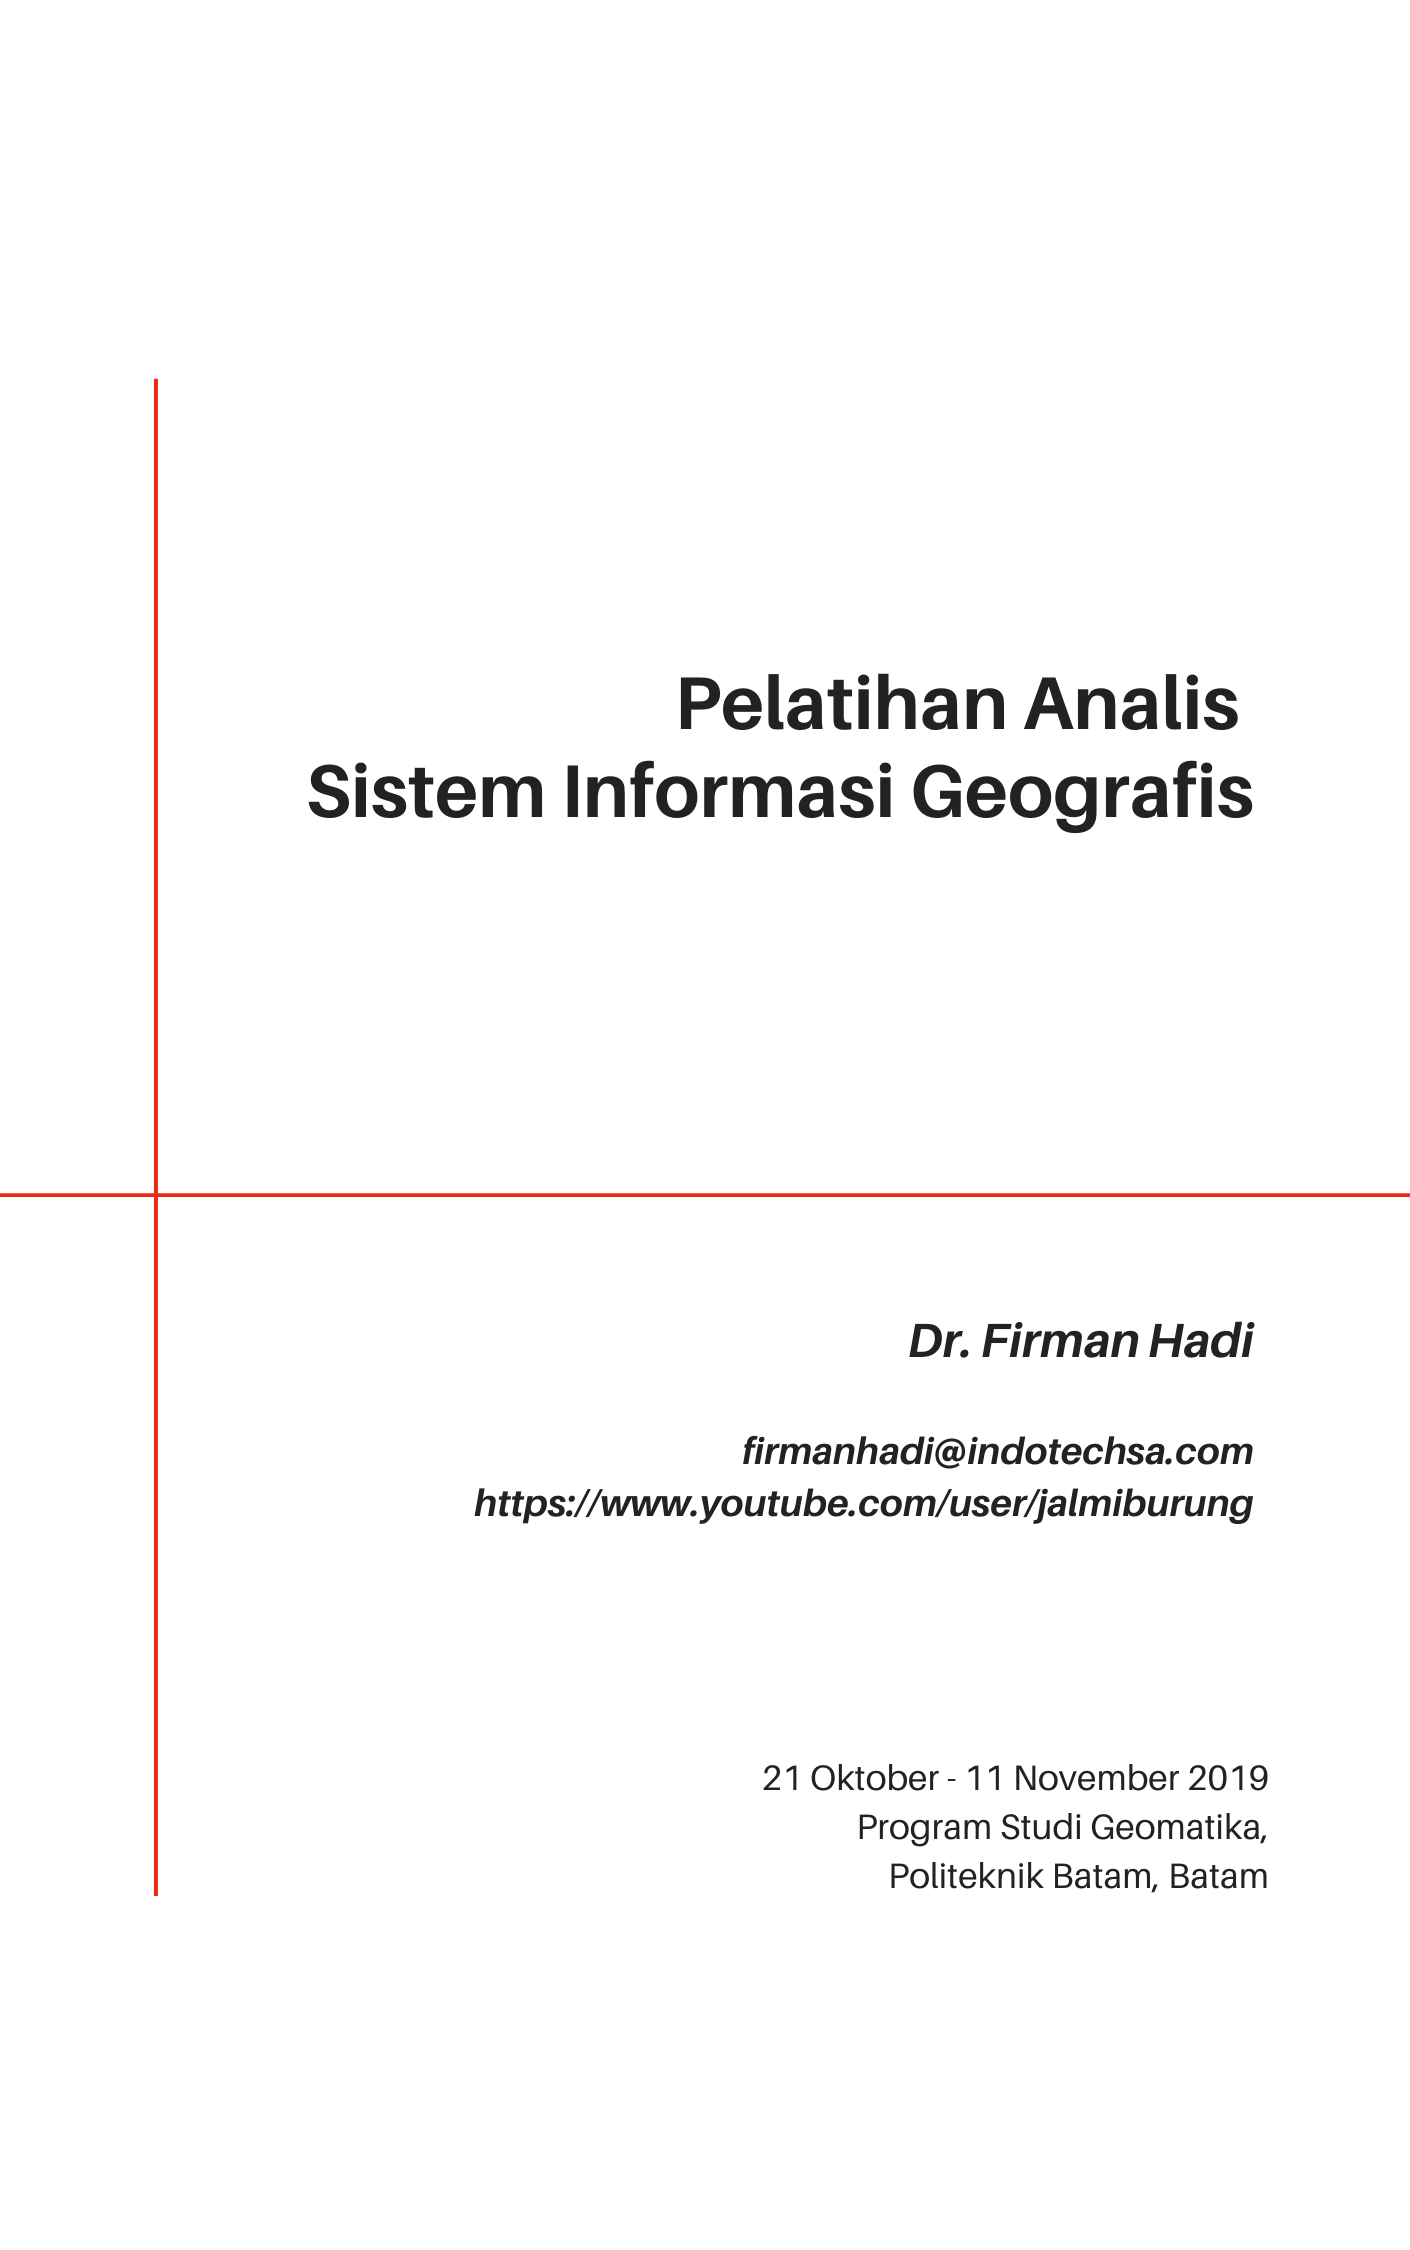
\includegraphics{cover.png}
\end{center}

{
\setcounter{tocdepth}{1}
\tableofcontents
}
\hypertarget{pengantar}{%
\chapter*{Pengantar}\label{pengantar}}
\addcontentsline{toc}{chapter}{Pengantar}

Repositori ini berisi kumpulan materi untuk Pelatihan Persiapan Uji Kompetensi Analis SIG yang dilaksanakan di Program Studi Teknik Geomatika, Politeknik Negeri Batam.

\hypertarget{part-basis-data}{%
\part{Basis Data}\label{part-basis-data}}

\hypertarget{day2}{%
\chapter{Basis Data}\label{day2}}

\hypertarget{perancangan-basis-data}{%
\section[Perancangan Basis Data ]{\texorpdfstring{Perancangan Basis Data \footnote{Sumber: \url{https://www.e-education.psu.edu/spatialdb/l2_p4.html}}}{Perancangan Basis Data }}\label{perancangan-basis-data}}

\hypertarget{rumusan-dasar}{%
\subsection{Rumusan Dasar}\label{rumusan-dasar}}

Dalam membangun basis data relasional dari awal, adalah penting untuk memberikan waktu lebih dalam memikirkan \textbf{\emph{business process}} yang terjadi. Basis data yang tidak dirancang dengan baik akan memberikan masalah bagi pengguna, termasuk :

\begin{itemize}
\tightlist
\item
  hilangnya integritas data seiring dengan waktu
\item
  ketidakmampuan dalam mendukung query yang diperlukan
\item
  performa yang buruk, misalnya, lambat dalam menampilkan hasil query
\end{itemize}

Rumusan dasar dalam merancang basis data adalah membuat tabel yang :

\begin{itemize}
\tightlist
\item
  meminimalisir data berlebih (redundant)
\item
  menggambarkan satu subyek
\item
  memiliki satu Primary Key (kode unik untuk setiap baris rekaman (record))
\item
  tidak mengandung kolom dengan banyak bagian (multi-part field) (Contoh: ``302 Walker Bldg, University Park, PA 16802'')
\item
  tidak mengandung kolom dengan ragam nilai (Contoh: Kolom Author hendaknya tidak berisi data seperti ``Jones, Martin, Williams'')
\item
  tidak memiliki duplikasi yang tidak perlu (Contoh: hindari penamaan kolom seperti Author1, Author2, Author3)
\item
  tidak memiliki kolom yang nilainya tergantung dari kolomm lain(Contoh: jangan membuat kolom gaji (Wage) untuk tabel yang memiliki kolom PayRate dan HrsWorked )
\end{itemize}

\hypertarget{normalisasi}{%
\subsection{Normalisasi}\label{normalisasi}}

Proses perancangan sebuah basis data seperti yang diuraikan dalam aturan di atas, secara formal disebut dengan normalisasi. Semua perancang basis data melakukan normalisasi, baik mereka menggunakan istilah tersebut untuk menggambarkan prosesnya atau tidak.

Ada tiga tingkatan normalisasi, yaitu :

\begin{itemize}
\tightlist
\item
  \textbf{First Normal Form (1NF)}
\end{itemize}

menggambarkan sebuah basis data yang tabel-tabelnya merepresentasikan entitas yang unik, tidak ada duplikasi kolom (misal, tidak ada Author1, Author2, Author3), memiliki satu atau banyak kolom yang merupakan identitas unik dari setiap baris (primary key, PK). Basis data yang memenuhi persyaratan ini termasuk ke dalam First Normal Form (1NF).

\begin{itemize}
\tightlist
\item
  \textbf{Second Normal Form (2NF)}
\end{itemize}

menggambarkan sebuah basis data yang dalam kondisi 1NF dan juga menghindari kolom non-key yang tergantung dari subset Primary Key. Silakan lihat penjelasan di tautan berikut untuk melihat contoh sederhananya {[}www.1keydata.com/database-normalization/second-normal-form-2nf.php{]}.

Dalam contoh di tautan tersebut, CustomerID dan StoreID membangun sebuah composite key (kunci gabungan) -- gabungan dari nilai kedua kolom tersebut bersifat unik, menjadi identitas setiap kolom dalam tabel. Dalam kata lain, hanya akan ada satu baris dalam tabel yang memiliki CustomerID 1 dengan StoreID 1, hanya akan ada satu baris dengan CustomerID 1 dan StoreID 3, dan seterusnya. Kolom PurchaseLocation tergantung dari kolom StoreID, yang merupakan sebagian dari Primary Key. Dengan demikian, solusi untuk menempatkan tabel ke dalam 2NF adalah dengan memindahkan hubungan StoreID-PurchaseLocation ke dalam tabel terpisah. Pendekatan ini bersifat intuitif di mana kita dapat membaca nilai PurchaseLocation satu kali dibandingkan berulang kali

\begin{itemize}
\tightlist
\item
  \textbf{Third Normal Form (3NF)}
\end{itemize}

menggambarkan sebuah basis data dalam tingkat 2NF dan juga menghindari kolom yang nilainya diturunkan dari kolom lain yang bukan Primary Key. Contoh kolom Wage seperti disebutkan di atas adalah sebuah pelanggaran aturan 3NF.

Dalam banyak kasus, normalisasi basis data hingga tingkatan 3NF sudah cukup. Perlu ditambahkan juga ada format normalisasi lain seperti Boyce-Codman Normal Form (BCNF, atau 3.5NF), Fourth Normal Form (4NF) dan Fifth Normal Form (5NF). Namun demikian, daripada membuang waktu lebih lama dalam menggambarkan normalisasi tingkat lanjut ini, yang paling simpel adalah mengingat karakteristik dasar dari sebuah tabel yang didesain secara baik seperti di atas. Apabila Anda mengikuti petunjuk tersebut secara seksama, khususnya secara konsisten mencari data berlebih (redundant), Anda akan mampu melakukan normalisasi basis data.

Singkatnya, semakin tinggi tingkatan normalisasi, maka akan semakin banyak jumlah tabel yang ada dalam basis data. Semakin banyak jumlah tabel, usaha untuk menggabungkan data dengan cara \emph{\textbf{joins}} juga akan semakin sulit, dalam arti semakin tinggi level keahlian yang diperlukan untuk membuat queri dan dalam meningkatkan performa basis data. Proses normalisasi kadang-kadang menghasilkan desain yang terlalu sulit untuk diimplementasikan atau kalaupun dapat dibuat, ia memiliki performa yang buruk (baca: lambat). Pada dasarnya, perancangan basis data adalah menyeimbangkan antara kebutuhan yang terkait dengan integritas data dan efisiensi penyimpanan data dengan kebutuhan yang terkait dengan penggunaannya (insert, update, query).

\textbf{Contoh}

Untuk memahami proses normalisasi basis data, contoh berikut memperlihatkan bagaimana aturan-aturan yang telah dijelaskan dapat diterapkan untuk menghasilkan sebuah basis data yang efisien. Pengusaha Jen dan Barry mengembangkan usaha es krim dan membutuhkan sebuah basis data untuk menjejak pesanan (order). Ketika menerima pesanan, mereka mencatat nama pelanggannya, detil pesanan seperti rasa (flavors) dan jumlah es krim yang dibutuhkan, tanggal pesanan dan alamat pengiriman pesanan. Basis data ini diharapkan dapat membantu mereka dalam menjawab dua penting sebagai berikut :

\begin{itemize}
\tightlist
\item
  Pesanan mana yang tenggatnya dalam 2 hari ke depan?
\item
  Perasa apa yang harus dibuat dalam jumlah yang lebih banyak?
\end{itemize}

Tabel pesanan yang dapat dibuat pertama kali adalah seperti gambar berikut :

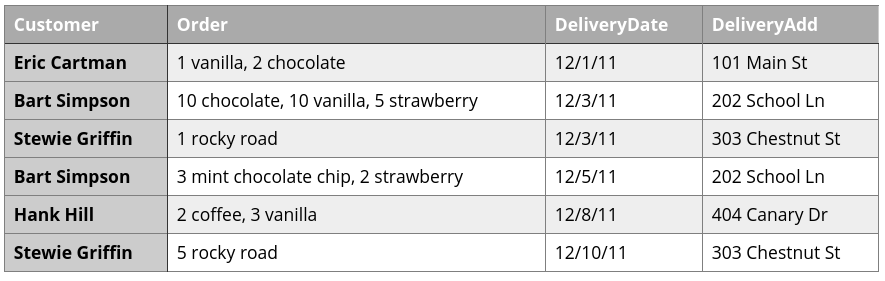
\includegraphics{./img/tab01_order.png}

Dengan skema di atas, masalah yang muncul adalah ketika mereka akan membuat sebuah query yang menghitung jumlah perasa vanilla yang diperlukan sesuai pesanan. Jumlahnya bercampur dengan nama perasa dan perasa apapun dapat dimasukkan ke dalam daftar di bagian mana saja (tidak akan konsisten dituliskan dalam kolom pertama atau kedua).

Oleh karenanya, desain seperti berikut sepertinya lebih baik:

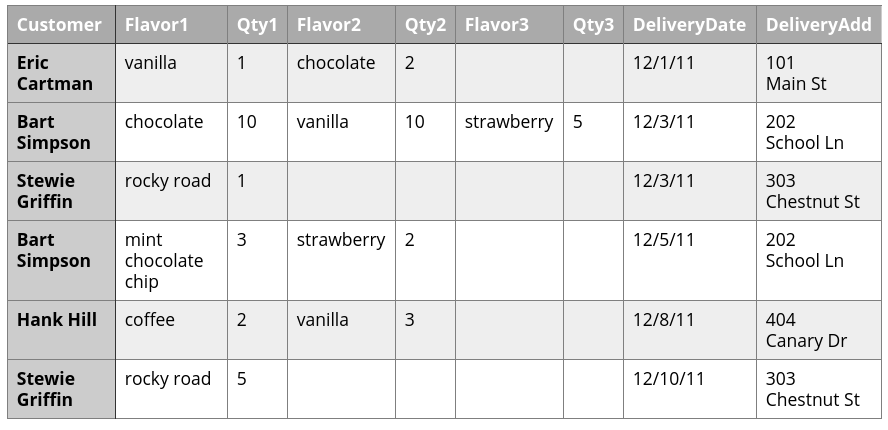
\includegraphics{./img/tab02a_order.png}
Skema yang kedua ini lebih baik karena memungkinkan mereka untuk melakukan query perasa tertentu dan menjumlahkan kuantitasnya. Namun untuk menghitung perasa vanila yang diperlukan, mereka harus menghitung jumlahnya dari tiga kolom berbeda. Desain ini juga tidak akan dapat menjawab permasalahan apabila satu orang pelanggan memesan lebih dari tiga perasa.

Desain seperti berikut mungkin menjawab pertanyaan di atas:

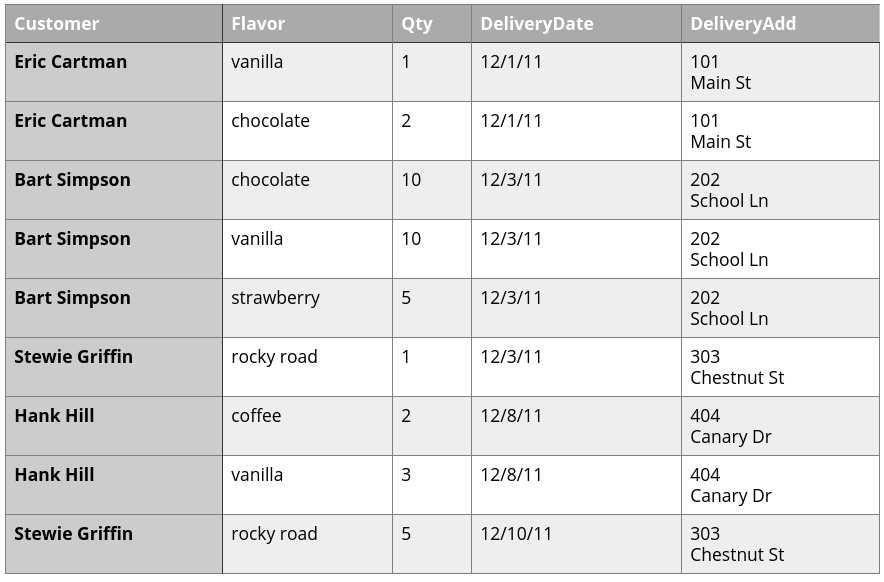
\includegraphics{./img/tab3_order.png}
Desain seperti di atas memungkinkan penghitungan kuantitas perasa vanila yang dibutuhkan sesuai pesanan dengan lebih mudah. Sayangnya, desain tersebut menghasilkan data berlebih (redundant) dan menuliskan pesanan dari satu pelanggan ke dalam banyak baris (record).

Desain yang paling baik adalah dengan memisahkan data ke dalam empat entitas (Customers, Flavors, Orders and Order Items):

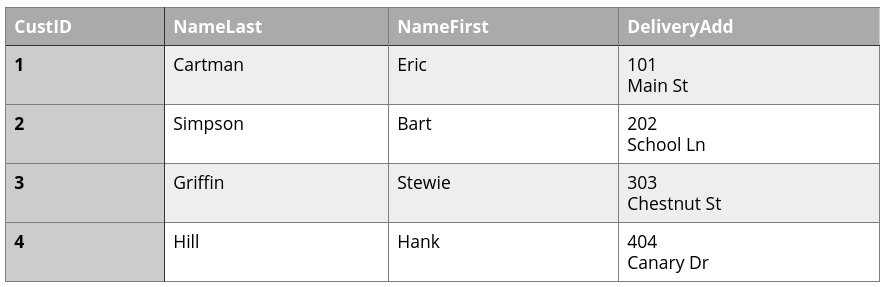
\includegraphics{./img/tab4_order.png}

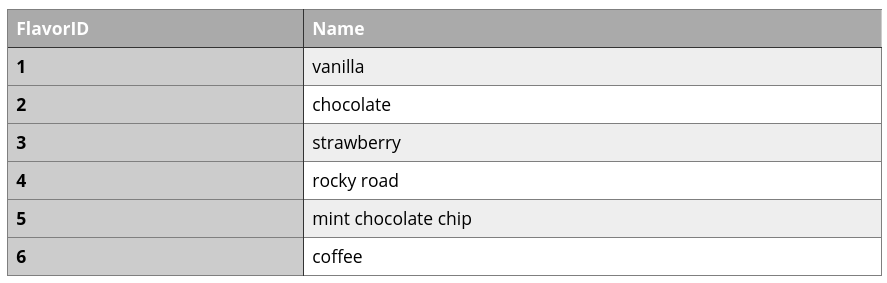
\includegraphics{./img/tab5_order.png}
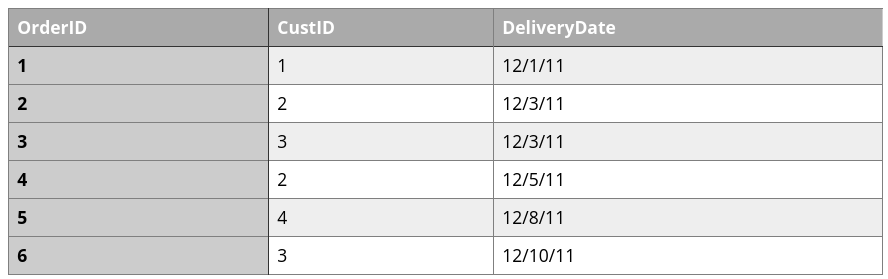
\includegraphics{./img/tab6_order.png}

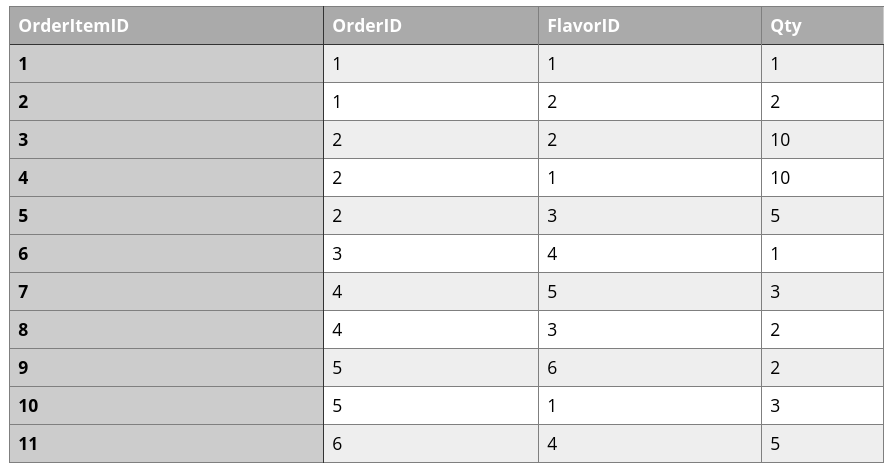
\includegraphics{./img/tab7_order.png}

Apabila mereka hendak mengimplementasikan desain seperti di atas dalam MS-Access, query yang diperlukan untuk menampilkan pesanan yang harus dikirim dalam 2 hari ke depan adalah seperti yang terlihat pada GUI :

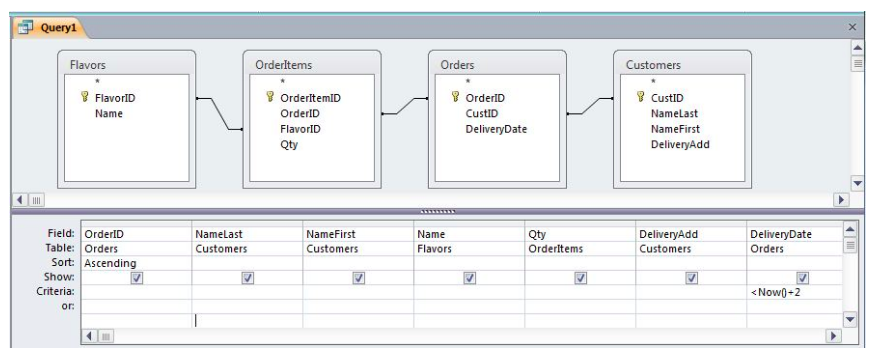
\includegraphics{./img/tab8_order.png}

\hypertarget{pemodelan-data}{%
\subsection{Pemodelan Data}\label{pemodelan-data}}

Pemodelan data dimulai dengan analisis kebutuhan, dapat dilakukan secara formal atau informal, tergantung dari skala proyeknya. Salah satu perangkat umum yang biasa digunakan dalam proses pemodelan adalah diagram entity-relationship (ER). Diagram ER mengilustrasikan kategori data yang harus disimpan (entitas), juga hubungan (relasi) antara entitas-entitas yang didefinisikan.

Model data menggambarkan entitas dunia nyata seperti pelanggan, layanan, produk, dan hubungan antara entitas ini. Model data menyediakan abstraksi untuk relasi dalam basis data. Model data membantu pengembang memodelkan persyaratan bisnis dan menerjemahkan persyaratan bisnis ke dalam relasi hubungan. Mereka juga digunakan untuk pertukaran informasi antara pengembang dan pemilik bisnis.

Di perusahaan, model data memainkan peran yang sangat penting dalam mencapai konsistensi data di seluruh sistem yang berinteraksi. Misalnya, jika suatu entitas tidak didefinisikan, atau tidak didefinisikan dengan baik, maka ini akan menyebabkan data yang tidak konsisten dan salah tafsir di seluruh perusahaan. Misalnya, jika semantik entitas pelanggan tidak didefinisikan dengan jelas, dan departemen bisnis yang berbeda menggunakan nama yang berbeda untuk entitas yang sama seperti pelanggan dan klien, ini dapat menyebabkan kebingungan di departemen operasional.

Perspektif model data didefinisikan oleh ANSI sebagai berikut:

\begin{itemize}
\tightlist
\item
  Model data konseptual:
\end{itemize}

Menjelaskan domain semantik, dan digunakan untuk mengkomunikasikan aturan utama dalam bisnis, aktor yang berperan, dan konsepnya. Ini menggambarkan persyaratan bisnis di tingkat tinggi dan sering disebut model data tingkat tinggi.

\begin{itemize}
\tightlist
\item
  Model data logis:
\end{itemize}

Menjelaskan semantik untuk teknologi tertentu, misalnya, diagram kelas UML untuk bahasa berorientasi objek.

\begin{itemize}
\tightlist
\item
  Model data fisik:
\end{itemize}

Menjelaskan bagaimana data sebenarnya disimpan dan dimanipulasi pada tingkat perangkat keras, seperti jaringan area penyimpanan, ruang tabel, CPU, dan sebagainya.

Menurut ANSI, abstraksi ini memungkinkan mengubah satu bagian dari tiga perspektif tanpa mengubah bagian lainnya. Seseorang dapat mengubah model data logis dan fisik tanpa mengubah model konseptual. Untuk menjelaskan, pengurutan data menggunakan gelembung atau pengurutan cepat tidak menarik untuk model data konseptual. Juga, mengubah struktur hubungan bisa transparan ke model konseptual. Seseorang dapat membagi satu relasi menjadi banyak relasi setelah menerapkan aturan normalisasi, atau dengan menggunakan tipe data enum untuk memodelkan tabel pencarian.

Model entitas-hubungan Model entitas-hubungan (ER) jatuh ke dalam kategori model data konseptual. Ini menangkap dan mewakili model data untuk pengguna bisnis dan pengembang. Model ER dapat ditransformasikan menjadi model relasional dengan mengikuti teknik-teknik tertentu.

Pemodelan konseptual adalah bagian dari siklus hidup pengembangan perangkat lunak (SDLC). Ini biasanya dilakukan setelah tahap pengumpulan-kebutuhan fungsional dan data. Pada titik ini, pengembang dapat membuat draf pertama diagram ER serta mendeskripsikan persyaratan fungsional menggunakan diagram aliran data, diagram urutan, cerita pengguna, dan banyak teknik lainnya.

Selama fase desain, pengembang basis data harus memberikan perhatian besar pada desain, menjalankan benchmark benchmark untuk memastikan kinerja, dan memvalidasi persyaratan pengguna. Pengembang memodelkan sistem sederhana bisa mulai mengkodekan secara langsung. Namun, kehati-hatian harus diambil ketika membuat desain, karena pemodelan data tidak hanya melibatkan algoritma dalam pemodelan aplikasi tetapi juga data. Perubahan dalam desain mungkin menyebabkan banyak kompleksitas di masa depan seperti migrasi data dari satu struktur data ke yang lain.

Saat merancang skema database, menghindari jebakan desain tidak cukup. Ada desain alternatif di mana seseorang dapat dipilih. Perangkap berikut harus dihindari:

Redundansi data: Desain database yang buruk menghasilkan data yang berlebihan. Data yang berlebihan dapat menyebabkan beberapa masalah lain, termasuk inkonsistensi data dan penurunan kinerja. Saat memperbarui tuple yang berisi data redundan, perubahan pada data redundan harus tercermin dalam semua tupel yang berisi data ini. Saturasi total: Secara alami, beberapa aplikasi memiliki data yang jarang, seperti aplikasi medis. Bayangkan suatu hubungan yang disebut diagnosa, yang memiliki ratusan atribut untuk gejala seperti demam, sakit kepala, bersin, dan sebagainya. Sebagian besar tidak valid untuk diagnosa tertentu, tetapi secara umum valid. Ini bisa dimodelkan dengan menggunakan tipe data yang kompleks seperti JSON. Kopling ketat: Dalam beberapa kasus, kopling ketat menyebabkan struktur data yang kompleks dan sulit diubah. Karena persyaratan bisnis berubah seiring waktu, beberapa persyaratan mungkin menjadi usang. Pemodelan generalisasi dan spesialisasi (misalnya, seorang siswa paruh waktu adalah seorang siswa) dengan cara yang digabungkan secara ketat dapat menyebabkan masalah.

Sebuah diagram ER pada basis adalah cetak biru dari satu struktur basis data. Beberapa RDBMS menyediakan perangkat untuk menggambar diagram ER (contohnya Oracle Designer, MySQL workbench, PostgreSQL pgModeler) dan juga terkadang menyediakan kemampuan untuk membuat struktur tabel yang telah dikonsepkan dalam bentuk diagram ke basis data.

Dalam konteks GIS, ESRI menyediakan perangkat yang memungkinkan kita membuat alat diagram geodatabase baru melalui CASE (Computer-Aided Software Engineering). Untuk lebih lanjutnya, Anda dapat membaca blog ini yang menjelaskan tentang penggunaan CASE, Menggunakan perkakas Case di Arc GIS 10, {[} \url{http://blogs.esri.com/esri/arcgis/2010/08/05/using-case-tools} -in-arcgis -10 /{]}.

\hypertarget{contoh-aplikasi}{%
\subsection{Contoh aplikasi}\label{contoh-aplikasi}}

Untuk menjelaskan dasar-dasar model ER, portal web online untuk membeli dan menjual mobil akan dimodelkan. Persyaratan aplikasi sampel ini adalah sebagai berikut, dan model ER akan dikembangkan langkah demi langkah:

Portal ini menyediakan fasilitas untuk mendaftarkan pengguna secara online dan menyediakan layanan yang berbeda untuk pengguna berdasarkan kategori mereka. Pengguna mungkin adalah penjual atau pengguna normal. Penjual dapat membuat iklan mobil baru; pengguna lain dapat menjelajahi dan mencari mobil. Semua pengguna harus memberikan nama lengkap dan alamat email yang valid saat pendaftaran. Alamat email akan digunakan untuk masuk. Penjual juga harus memberikan alamat. Pengguna dapat menilai iklan dan kualitas layanan penjual. Riwayat pencarian semua pengguna harus dipertahankan untuk digunakan nanti. Penjual memiliki peringkat dan ini mempengaruhi pencarian iklan; peringkat ditentukan oleh jumlah iklan yang dipasang dan peringkat pengguna. Iklan mobil memiliki tanggal dan mobil dapat memiliki banyak atribut seperti warna, jumlah pintu, jumlah pemilik sebelumnya, nomor registrasi, gambar, dan sebagainya. Entitas, atribut, dan kunci. Diagram ER mewakili entitas, atribut, dan hubungan. Entitas adalah representasi dari objek dunia nyata seperti mobil atau pengguna. Atribut adalah properti dari suatu objek dan menggambarkannya. Hubungan mewakili hubungan antara dua atau lebih entitas.

Atribut mungkin komposit atau sederhana (atom). Atribut komposit dapat dibagi menjadi beberapa bagian yang lebih kecil. Subbagian dari atribut gabungan memberikan informasi yang tidak lengkap yang secara semantik tidak berguna dengan sendirinya. Misalnya, alamat terdiri dari nama jalan, nomor gedung, dan kode pos. Salah satu dari mereka tidak berguna sendirian, tanpa rekan-rekannya.

Atribut juga bisa bernilai tunggal atau multi-nilai. Warna burung adalah contoh atribut multi-nilai. Itu bisa merah dan hitam, atau kombinasi dari warna lain. Atribut multi-nilai dapat memiliki batas bawah dan atas untuk membatasi jumlah nilai yang diizinkan. Selain itu, beberapa atribut dapat diturunkan dari atribut lainnya. Usia dapat diturunkan dari tanggal lahir. Dalam contoh kami, peringkat akhir penjual berasal dari jumlah iklan dan peringkat pengguna.

Atribut kunci dapat mengidentifikasi entitas di dunia nyata. Atribut kunci harus ditandai sebagai atribut unik, tetapi tidak harus sebagai kunci primer, ketika memodelkan relasi secara fisik. Akhirnya, beberapa tipe atribut dapat dikelompokkan bersama untuk membentuk atribut yang kompleks:

\begin{figure}

{\centering 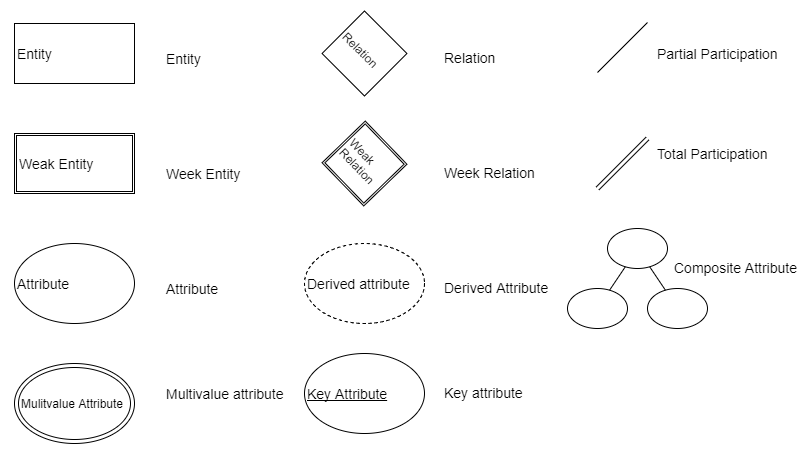
\includegraphics[width=0.7\linewidth]{img/01/db_model1} 

}

\caption{Simbol Entitas }\label{fig:fig11}
\end{figure}

Entitas harus memiliki nama dan seperangkat atribut. Mereka diklasifikasikan menjadi sebagai berikut:

Entitas lemah: Tidak memiliki atribut kunci dari entitas Kuatnya sendiri / entitas reguler: Memiliki atribut kunci Entitas yang lemah biasanya terkait dengan entitas yang kuat. Entitas yang kuat ini disebut entitas pengidentifikasi. Entitas yang lemah memiliki kunci parsial, juga dikenal sebagai diskriminator, yang merupakan atribut yang secara unik dapat mengidentifikasi entitas yang lemah, dan terkait dengan entitas yang mengidentifikasi. Dalam contoh kami, jika kami menganggap bahwa kunci pencarian berbeda setiap kali pengguna mencari mobil, maka kunci pencarian adalah kunci parsial. Simbol entitas yang lemah dibedakan dengan mengelilingi kotak entitas dengan garis ganda.

Diagram berikut menunjukkan desain awal aplikasi portal mobil. Entitas pengguna memiliki beberapa atribut. Atribut nama adalah atribut gabungan, dan email adalah atribut kunci. Entitas penjual adalah spesialisasi entitas pengguna. Peringkat total adalah atribut turunan yang dihitung dengan menggabungkan peringkat pengguna dan jumlah iklan. Atribut warna mobil ini bernilai multi. Penjual dapat dinilai oleh pengguna untuk iklan tertentu; hubungan ini adalah hubungan terner, karena peringkat melibatkan tiga entitas, yaitu mobil, penjual, dan pengguna.

Gambar mobil adalah atribut sub bagian dari iklan. Diagram berikut menunjukkan bahwa mobil dapat diiklankan lebih dari satu kali oleh penjual yang berbeda. Di dunia nyata, ini masuk akal, karena orang dapat meminta lebih dari satu penjual untuk menjual mobilnya:

\begin{center}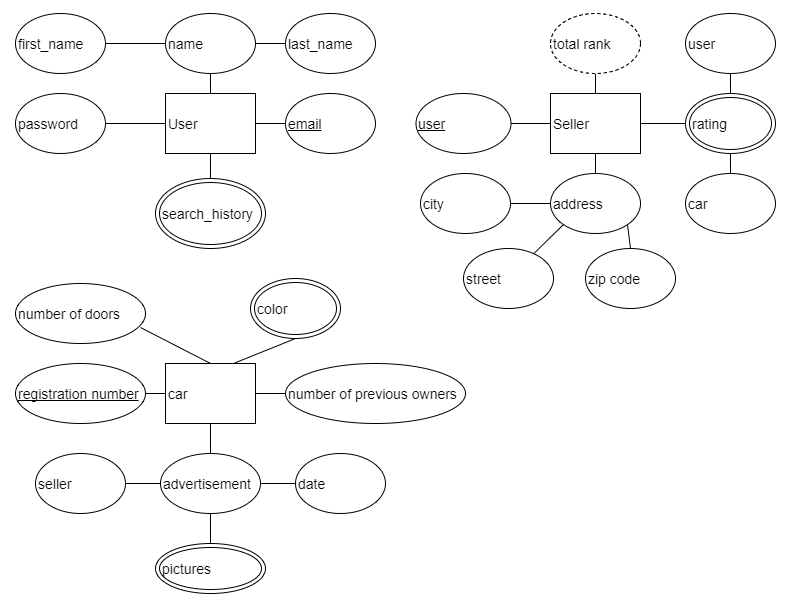
\includegraphics[width=0.7\linewidth]{img/01/db_model2} \end{center}

Ketika atribut dari satu entitas merujuk ke entitas lain, beberapa hubungan ada. Dalam model ER, referensi ini tidak boleh dimodelkan sebagai atribut tetapi sebagai hubungan atau entitas yang lemah. Mirip dengan entitas, ada dua kelas hubungan: lemah dan kuat. Hubungan yang lemah mengasosiasikan entitas yang lemah dengan entitas lain. Hubungan dapat memiliki atribut sebagai entitas. Dalam contoh kita, mobil diiklankan oleh penjual; tanggal iklan adalah properti hubungan.

Hubungan memiliki batasan kardinalitas untuk membatasi kemungkinan kombinasi entitas yang berpartisipasi dalam suatu hubungan. Batasan utama mobil dan penjual adalah 1: N; mobil diiklankan oleh satu penjual, dan penjual dapat mengiklankan banyak mobil. Partisipasi antara penjual dan pengguna disebut partisipasi total, dan dilambangkan dengan garis ganda. Ini berarti bahwa penjual tidak dapat hidup sendiri, dan ia harus menjadi pengguna.

Catatan

Batasan hubungan kardinalitas banyak-ke-banyak dilambangkan dengan N: M untuk menekankan perbedaan partisipasi oleh entitas.

\begin{center}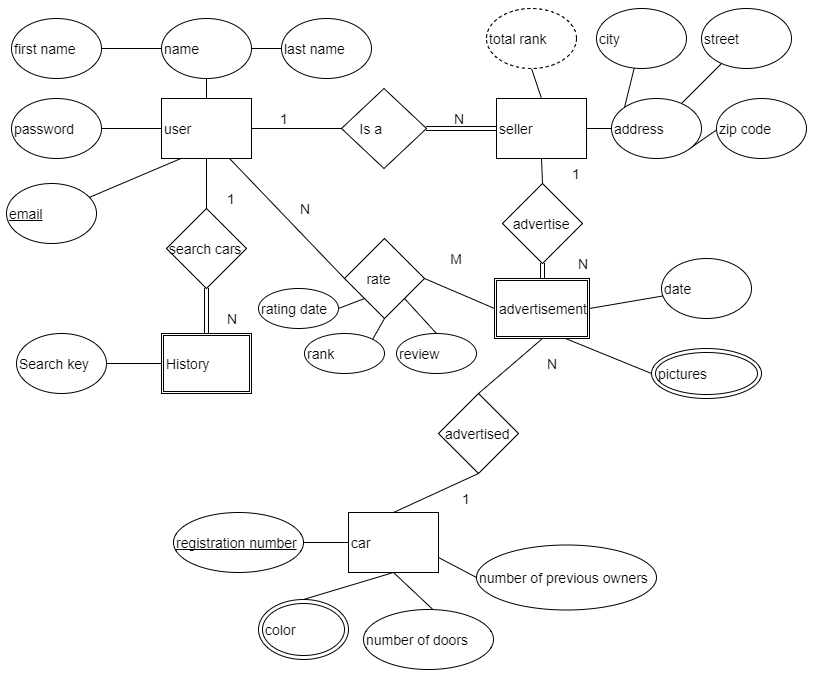
\includegraphics[width=0.7\linewidth]{img/01/db_model3} \end{center}

Sampai sekarang, hanya konsep dasar diagram ER yang telah dibahas. Beberapa konsep, seperti notasi kardinalitas (min, maks), hubungan ternary / n-ary, generalisasi, spesialisasi, dan diagram entity entity (EER) yang disempurnakan, belum pernah dibahas.

Memetakan ER ke relasi Aturan untuk memetakan diagram ER ke sekumpulan relasi (yaitu, skema basis data) hampir mudah, tetapi tidak kaku. Orang bisa memodelkan entitas sebagai atribut, dan kemudian memperbaikinya menjadi suatu hubungan. Atribut yang dimiliki beberapa entitas dapat dipromosikan menjadi entitas independen. Aturan yang paling umum adalah sebagai berikut (perhatikan bahwa hanya aturan dasar yang telah dicakup, dan daftarnya tidak lengkap):

Memetakan entitas biasa ke hubungan. Jika entitas memiliki atribut gabungan, maka sertakan semua bagian dari atribut. Pilih salah satu atribut kunci sebagai kunci utama. Memetakan entitas yang lemah ke hubungan. Sertakan atribut sederhana dan sub bagian dari atribut komposit. Tambahkan kunci asing untuk referensi entitas yang mengidentifikasi. Kunci primer biasanya merupakan kombinasi dari kunci parsial dan kunci asing.

Jika suatu hubungan memiliki atribut dan kardinalitas relasinya adalah 1: 1, maka atribut relasi tersebut dapat ditetapkan ke salah satu entitas yang berpartisipasi. Jika suatu hubungan memiliki atribut dan kardinalitas relasinya adalah 1: N, maka atribut relasi dapat ditetapkan ke entitas yang berpartisipasi di sisi N. Peta banyak-ke-banyak hubungan, juga dikenal sebagai N: M, ke hubungan baru. Tambahkan kunci asing untuk referensi entitas yang berpartisipasi. Kunci utama adalah komposisi kunci asing. Memetakan atribut multi-nilai ke suatu relasi. Tambahkan kunci asing untuk referensi entitas yang memiliki atribut multi-nilai. Kunci utama adalah komposisi kunci asing dan atribut multi-nilai.

Diagram kelas UML Unified Modeling Language (UML) adalah standar yang dikembangkan oleh Object Management Group (OMG). Diagram UML banyak digunakan dalam pemodelan solusi perangkat lunak, dan ada beberapa jenis diagram UML untuk berbagai tujuan pemodelan termasuk kelas, use case, aktivitas, dan diagram implementasi. Diagram kelas UML Unified Modeling Language (UML) adalah standar yang dikembangkan oleh Object Management Group (OMG).

Diagram UML banyak digunakan dalam pemodelan solusi perangkat lunak, dan ada beberapa jenis diagram UML untuk berbagai tujuan pemodelan termasuk kelas, use case, aktivitas, dan diagram implementasi. Diagram kelas UML Unified Modeling Language (UML) adalah standar yang dikembangkan oleh Object Management Group (OMG). Diagram UML banyak digunakan dalam pemodelan solusi perangkat lunak, dan ada beberapa jenis diagram UML untuk berbagai tujuan pemodelan termasuk kelas, use case, aktivitas, dan diagram implementasi.

Diagram kelas dapat mewakili beberapa jenis asosiasi, yaitu hubungan antar kelas. Mereka dapat menggambarkan atribut serta metode. Diagram ER dapat dengan mudah diterjemahkan ke dalam diagram kelas UML. Diagram kelas UML juga memiliki keuntungan sebagai berikut:

Rekayasa ulang kode: Skema basis data dapat dengan mudah dibalik untuk menghasilkan diagram kelas UML. Pemodelan objek basis data relasional yang diperluas: Database relasional modern memiliki beberapa jenis objek seperti sekuens, tampilan, indeks, fungsi, dan prosedur tersimpan. Diagram kelas UML memiliki kemampuan untuk mewakili jenis objek ini. Diagram kelas berikut dihasilkan dari rekayasa ulang kode SQL dari car\_portaldatabase:

\begin{center}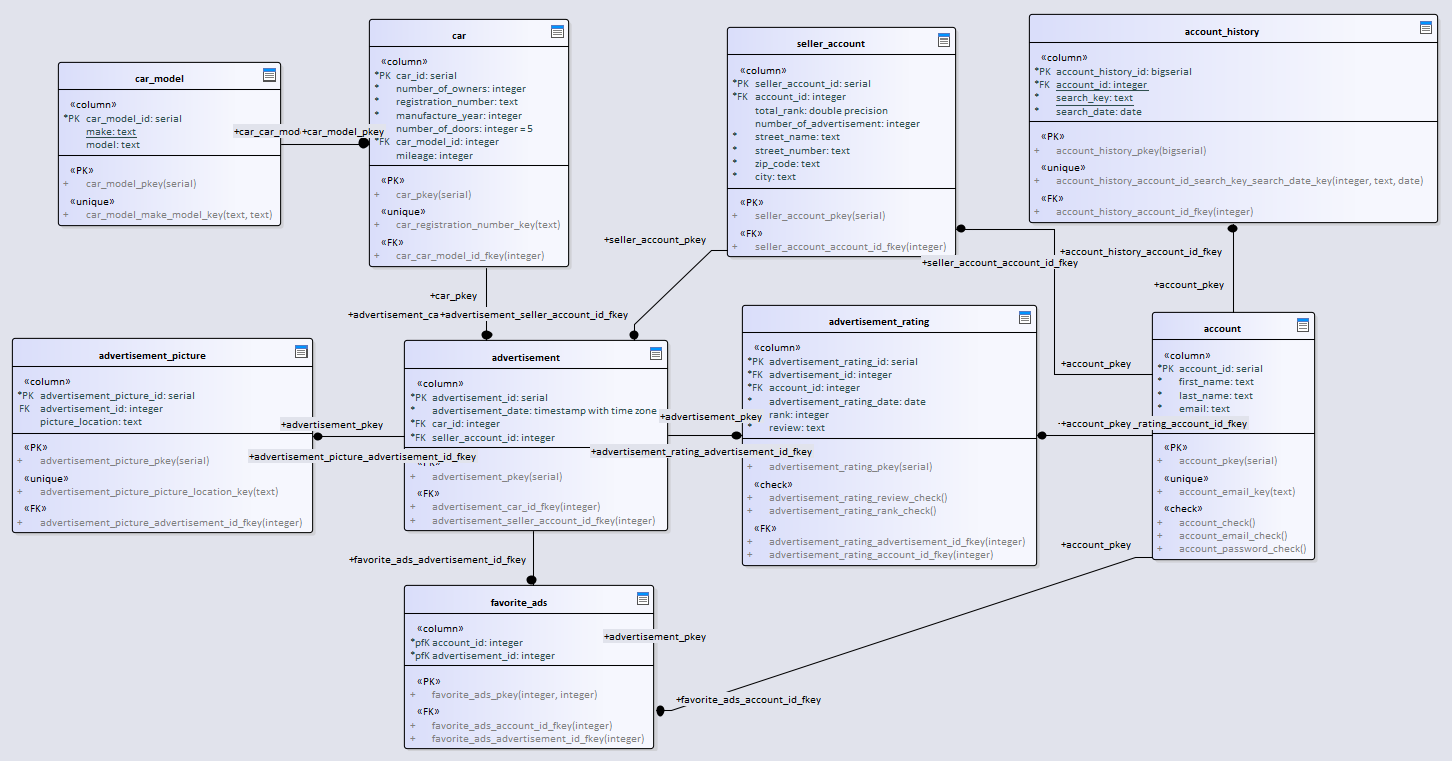
\includegraphics[width=0.9\linewidth]{img/01/db_model4} \end{center}

\hypertarget{pembuatan-basis-data-dengan-postgis}{%
\section[Pembuatan Basis Data dengan PostGIS ]{\texorpdfstring{Pembuatan Basis Data dengan PostGIS \footnote{Sumber: \url{https://github.com/andyprasetya/webmap-development-server}}}{Pembuatan Basis Data dengan PostGIS }}\label{pembuatan-basis-data-dengan-postgis}}

\hypertarget{membuat-skema-baru-dengan-pgadmin-4}{%
\subsection{Membuat Skema Baru dengan pgAdmin 4}\label{membuat-skema-baru-dengan-pgadmin-4}}

Instalasi \textbf{PgAdmin 4} sangat mudah. Anda tinggal men-\emph{download}-nya dari \href{https://www.pgadmin.org/download/}{download page} di situsnya, dan laksanakan proses instalasi di \textbf{workstation} hingga selesai. Sebagai catatan, Anda akan diminta untuk membuat \textbf{master password}, yaitu \emph{password} yang digunakan saat pertama kali mengakses \textbf{PgAdmin 4} di \emph{workstation} Anda.

\begin{figure}
\centering
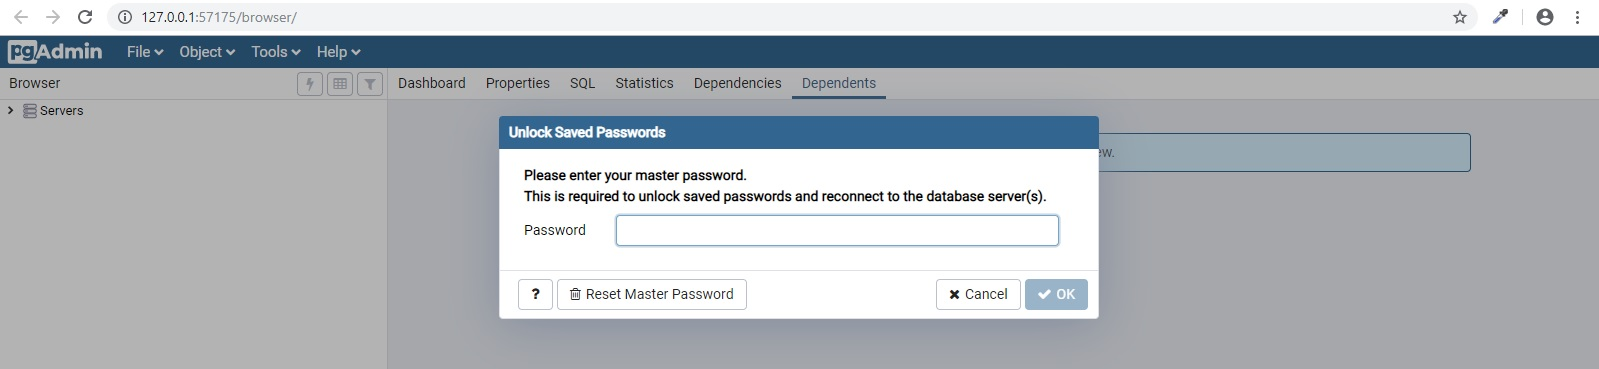
\includegraphics{./img/pgadmin4-master-password.jpg}
\caption{PgAdmin 4}
\end{figure}

Setelah Anda berhasil masuk ke \textbf{PgAdmin 4}, maka yang pertama kali harus dilakukan adalah \emph{create connection} ke server PostgreSQL yang akan Anda akses.

\begin{figure}
\centering
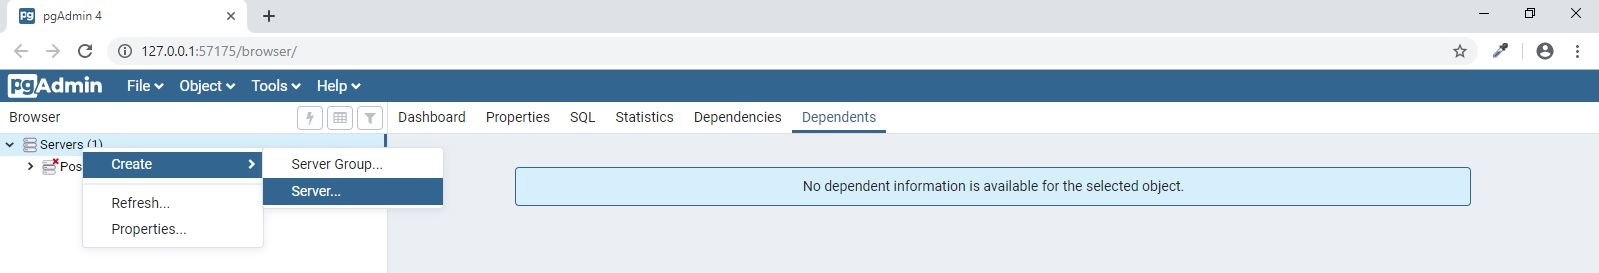
\includegraphics{./img/pgadmin4-create.jpg}
\caption{PgAdmin 4}
\end{figure}

Pada \emph{dialog} ini, di \emph{tab} \textbf{General} kita isi \textbf{Name} dengan \textbf{Webmap Development Server} (atau sesuka Anda), kemudian \emph{checkbox} \textbf{Connect now?}-nya kita \emph{check}, dan \textbf{Comments}-nya kita isi dengan deskripsi koneksinya.

\begin{figure}
\centering
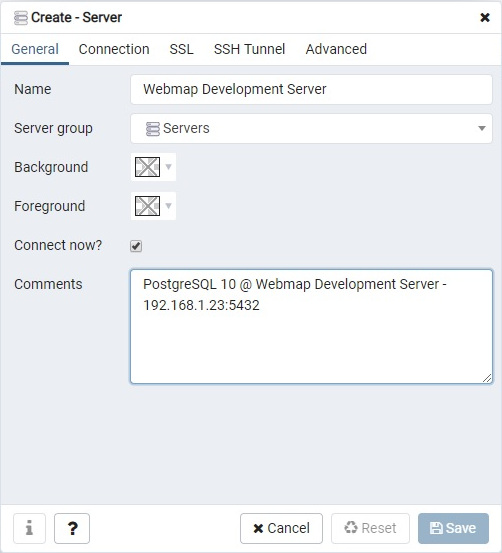
\includegraphics{./img/pgadmin4-create-general.jpg}
\caption{PgAdmin 4}
\end{figure}

Pindah ke \emph{tab} \textbf{Connection}, kita isi \textbf{Host name/address} dengan \textbf{192.168.1.23} (IP server PostgreSQL-nya), \textbf{Port}: \textbf{5432}, \textbf{Username}: \textbf{pgdbadmin} (biar bisa mengakses seluruh database yang ada), dan \emph{password}-nya. \emph{Checkbox} Save \textbf{Password?}-nya boleh di-\emph{check}, tapi lebih baik dibiarkan \emph{unchecked} saja, sehingga setiap kali koneksi Anda akan diminta untuk memasukkan \emph{password}.

\begin{figure}
\centering
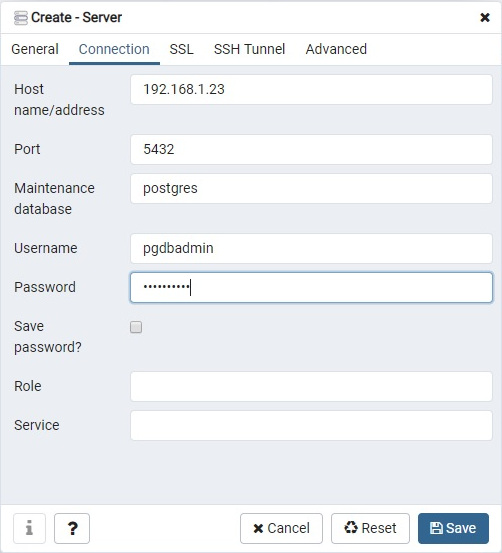
\includegraphics{./img/pgadmin4-create-connection.jpg}
\caption{PgAdmin 4}
\end{figure}

Kalau seluruh isian kita sudah benar, maka begitu kita klik \textbf{Save}, maka entry \textbf{Webmap Development Server} akan muncul di pilihan server pada \textbf{PgAdmin 4}:

\begin{figure}
\centering
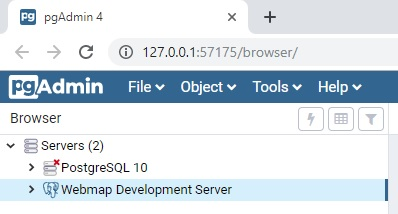
\includegraphics{./img/pgadmin4-connection-created.jpg}
\caption{PgAdmin 4}
\end{figure}

Waktu kita \emph{unfold entry} ini, maka akan muncul pilihan akses ke \textbf{Databases}, \textbf{Login/Group Roles} dan \textbf{Tablespaces}. Selanjutnya, kita akan fokus ke \textbf{Databases} dulu.

\begin{figure}
\centering
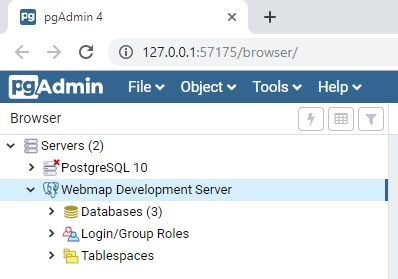
\includegraphics{./img/pgadmin4-connection-collapsed.jpg}
\caption{PgAdmin 4}
\end{figure}

Setelah kita \emph{unfold} \textbf{Databases}, maka akan terlihat \textbf{3} \emph{database}, yaitu \textbf{postgres} (\emph{default database}, yang digunakan oleh PostgreSQL), \textbf{postgis\_template} (\emph{database} yang sudah kita \emph{create} sebelumnya dan kita fungsikan sebagai \emph{template database}) dan \textbf{webmap\_db} (\emph{database} yang akan kita akses selanjutnya).

\begin{figure}
\centering
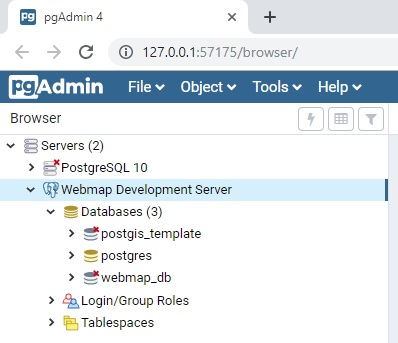
\includegraphics{./img/pgadmin4-collapsed-show-db.jpg}
\caption{PgAdmin 4}
\end{figure}

Masuk ke \textbf{webmap\_db} -\textgreater{} \textbf{Schemas} -\textgreater{} \textbf{public} -\textgreater{} \textbf{Tables}, maka akan terlihat \emph{table} bernama \textbf{ne\_10m\_admin\_0\_countries}, yang mana itu adalah hasil \emph{upload} shapefile yang sudah kita laksanakan pada bagian sebelumnya.

\begin{figure}
\centering
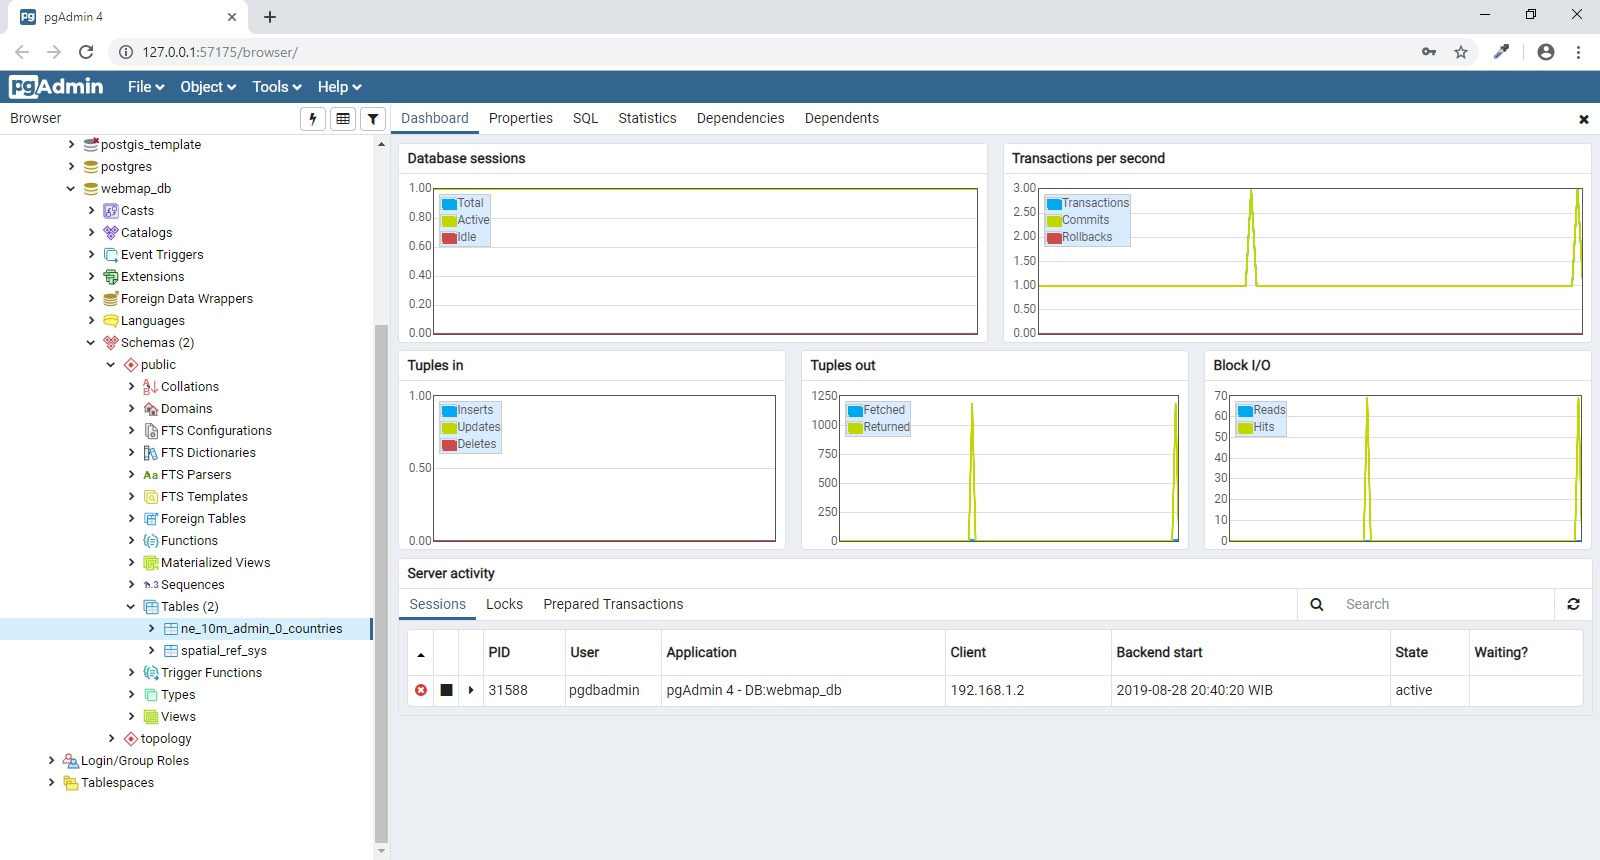
\includegraphics{./img/pgadmin4-show-tables.jpg}
\caption{PgAdmin 4}
\end{figure}

Klik-kanan pada \emph{table} tersebut (\textbf{\emph{ne\_10m\_admin\_0\_countries}}), pilih \textbf{View/Edit Data} -\textgreater{} \textbf{All Rows}:

\begin{figure}
\centering
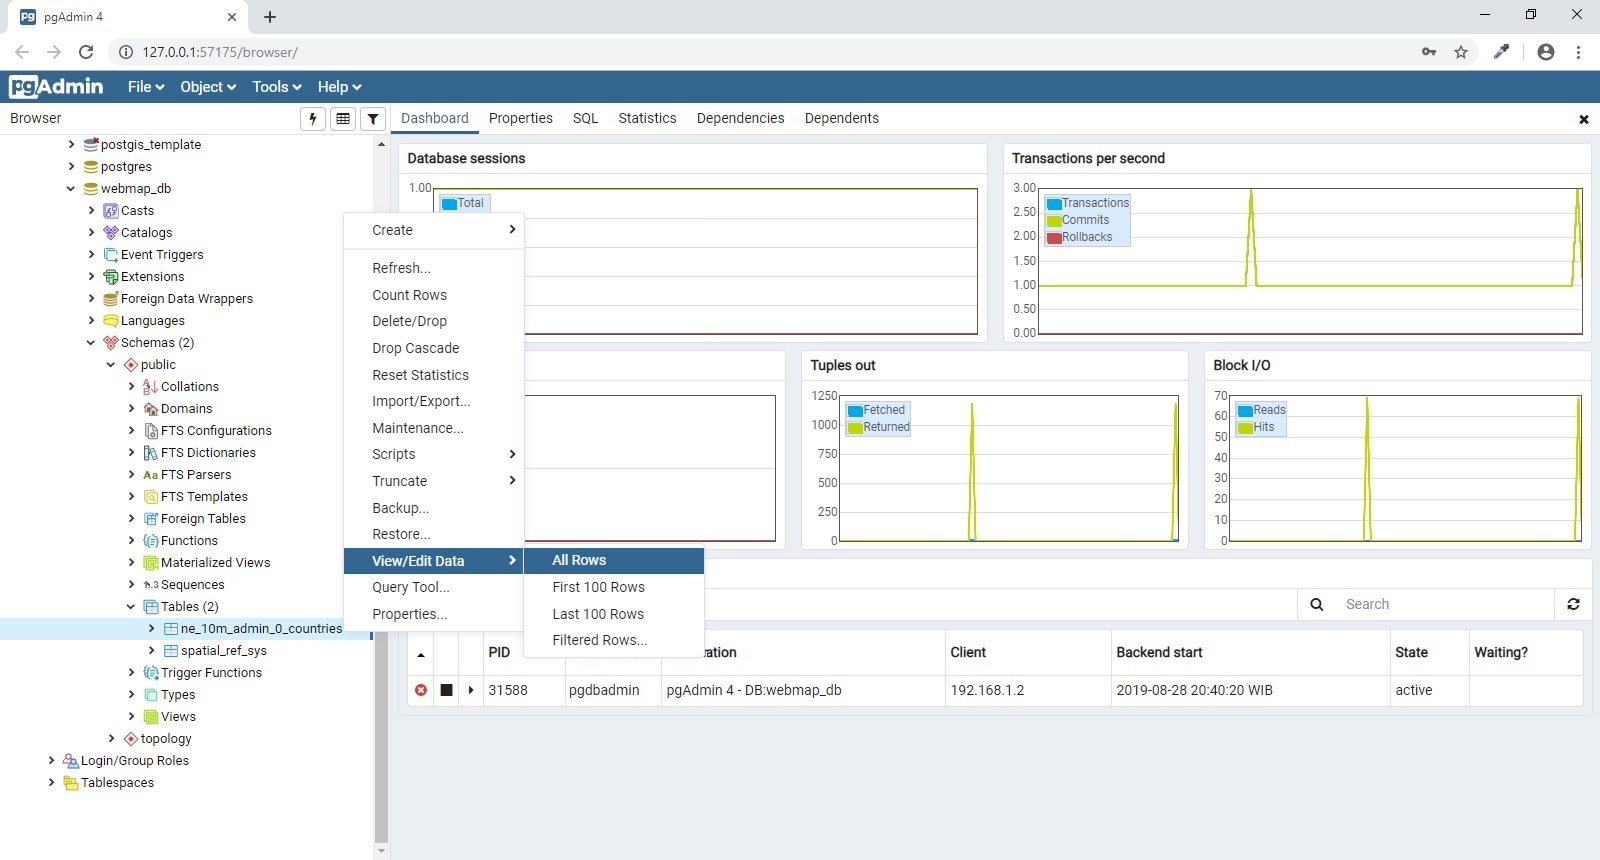
\includegraphics{./img/pgadmin4-right-click-on-table.jpg}
\caption{PgAdmin 4}
\end{figure}

Maka selanjutnya pada bagian kanan (tampilan utama) dari PgAdmin 4 akan muncul tampilan \emph{query} dan seluruh \emph{rows} yang ada dalam \emph{table} \textbf{\emph{ne\_10m\_admin\_0\_countries}}.

\begin{figure}
\centering
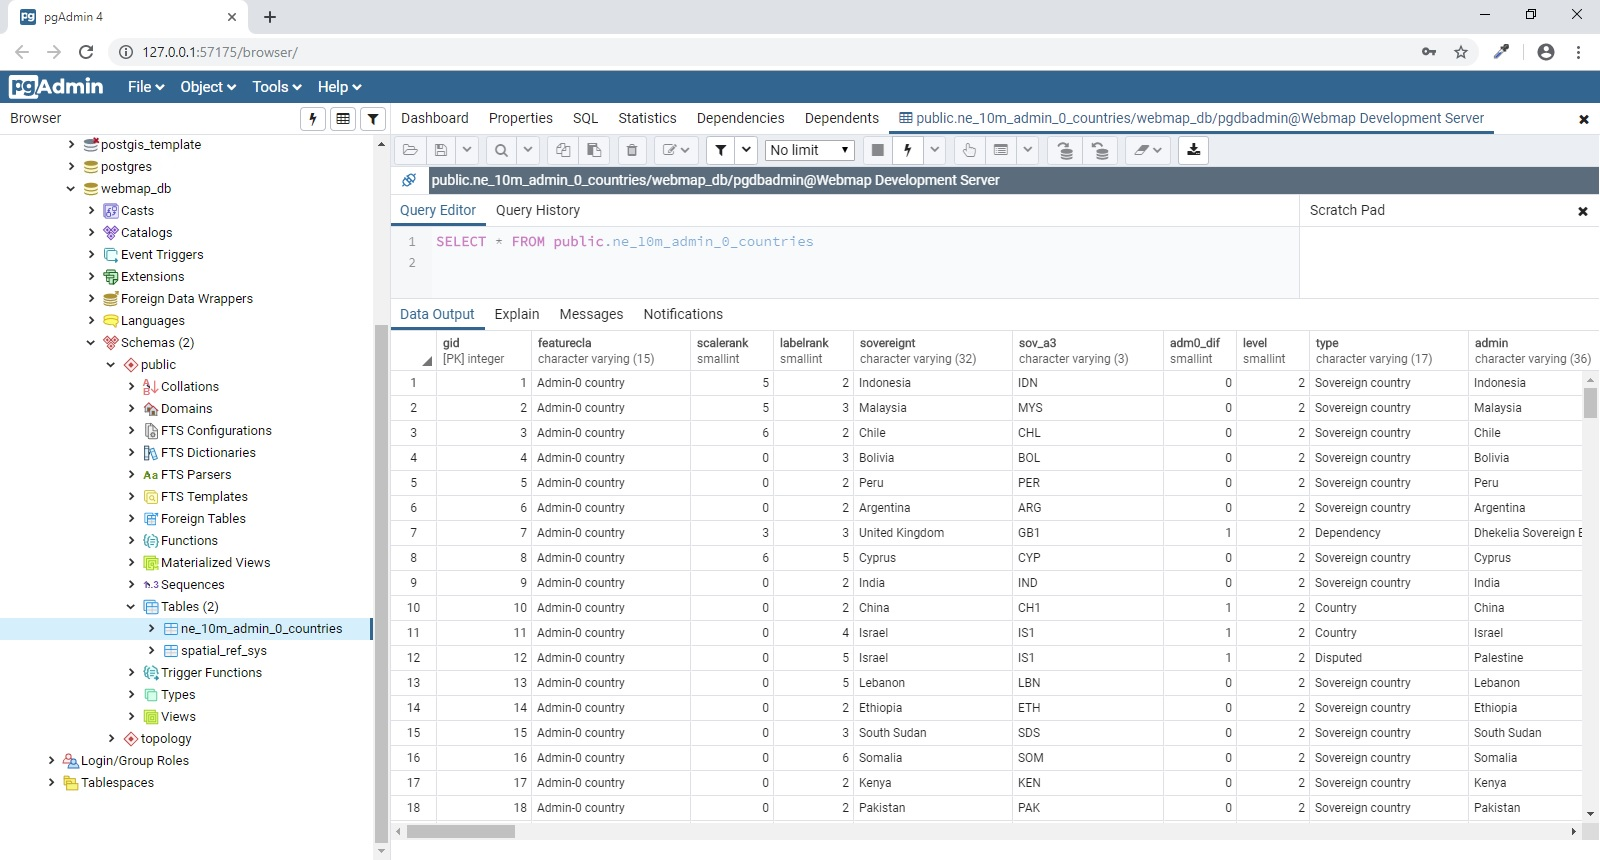
\includegraphics{./img/pgadmin4-show-all-entries.jpg}
\caption{PgAdmin 4}
\end{figure}

Menariknya pada \textbf{PgAdmin 4} ini, jika Anda \emph{scroll} ke kanan terus hingga akhir \emph{table}, akan ada sebuah \emph{button} yang berfungsi untuk menampilkan/visualisasi data \emph{geometry}-nya.

\begin{figure}
\centering
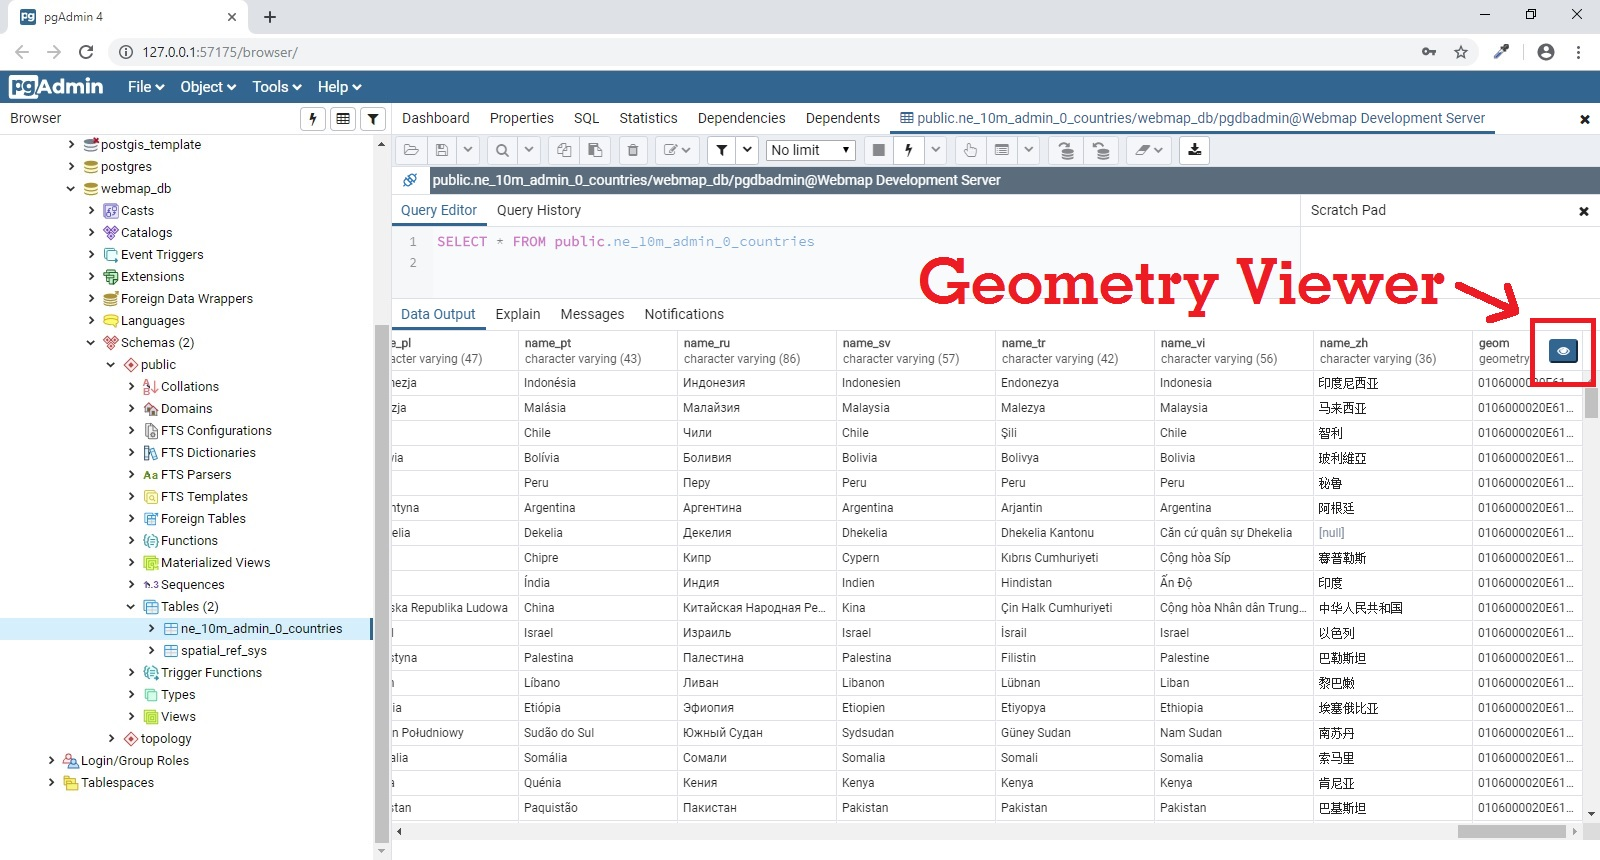
\includegraphics{./img/pgadmin4-geometry-viewer-button.jpg}
\caption{PgAdmin 4}
\end{figure}

Kalau di-klik \emph{geometry viewer button} ini, maka selanjutnya akan muncul \emph{webmap} berbasis \href{https://leafletjs.com/}{\textbf{Leaflet.JS}} yang menampilkan data \emph{geometry}-nya.

\begin{figure}
\centering
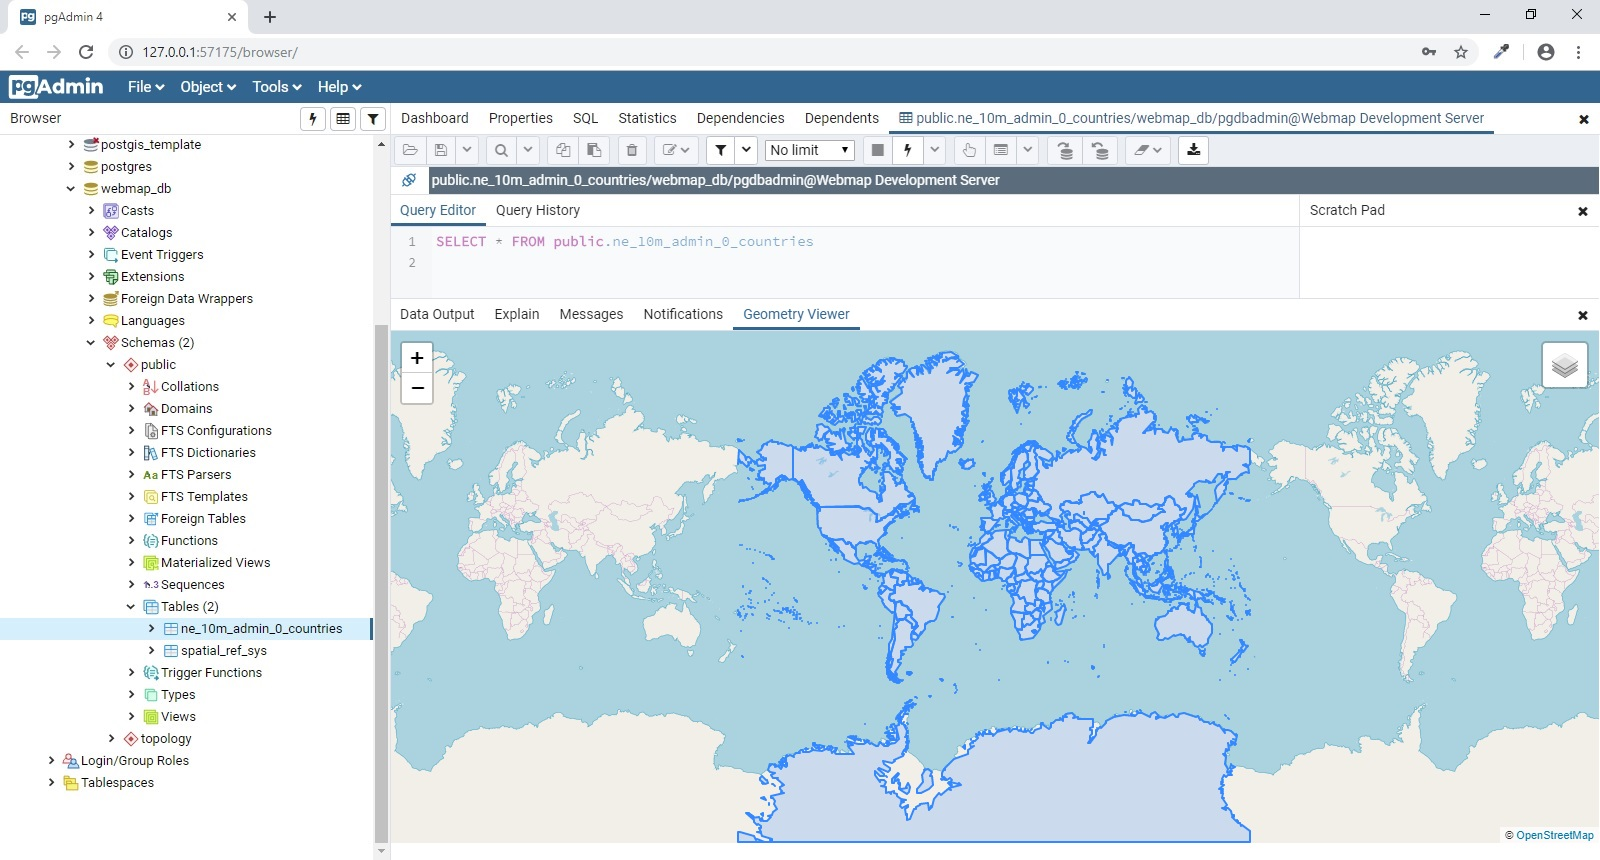
\includegraphics{./img/pgadmin4-geometry-viewer-map.jpg}
\caption{PgAdmin 4}
\end{figure}

Sebagai catatan, \emph{basemap} dari \href{}{\textbf{OpenStreetMap}} hanya akan muncul apabila SRID-nya \textbf{EPSG 4326}. Saya belum mencoba untuk \textbf{EPSG 3857} atau lainnya. Untuk lebih jelasnya mengenai perbedaan antara \textbf{EPSG 4326} dan \textbf{EPSG 3857}, dapat Anda baca di artikel bertajuk \href{https://lyzidiamond.com/posts/4326-vs-3857}{EPSG 4326 vs EPSG 3857} ini.

\hypertarget{postgis-shapefile-and-dbf-loaderexporter}{%
\subsection{PostGIS Shapefile and DBF Loader/Exporter}\label{postgis-shapefile-and-dbf-loaderexporter}}

Lakukan langkah-langkah ini di workstation Anda.

FYI, PostGIS Shapefile and DBF Loader/Exporter adalah sebuah aplikasi sederhana yang menjadi bagian dari paket instalasi PostGIS. Instalasi PostGIS membutuhkan PostgreSQL yang sudah terinstall (dan aktif) sebelumnya. Nah, menurut opini saya, instalasi PostgreSQL dan PostGIS di workstation \emph{nggak} berguna, kecuali hanya untuk \emph{``memancing''} instalasi \textbf{Application Stack Builder}, biar bisa install PostGIS yang mana di proses instalasinya akan mengikutkan \textbf{PostGIS Shapefile and DBF Loader Exporter}. PostgreSQL dan PostGIS \emph{toh} sudah ada di server. Tapi ya\ldots{} mau \emph{gimana} lagi? \emph{Let's just do it!}

\begin{itemize}
\item
  \href{https://www.enterprisedb.com/downloads/postgres-postgresql-downloads}{\textbf{\emph{Download}}} installer PostgreSQL dari EnterpriseDB/EDB, dan install sampai selesai.

  \begin{quote}
  Jika Anda akan langsung melakukan shapefile \emph{upload test}, Anda bisa men-\emph{download} 1 file dari situs \href{https://www.naturalearthdata.com/}{\textbf{Natural Earth}}. Ambil contoh, \href{https://www.naturalearthdata.com/http//www.naturalearthdata.com/download/10m/cultural/ne_10m_admin_0_countries.zip}{\textbf{batas administrasi negara level 0}}.
  \end{quote}
\item
  Setelah instalasi PostgreSQL selesai, dari \emph{Start menu} jalankan \textbf{Application Stack Builder}.

  \begin{figure}
  \centering
  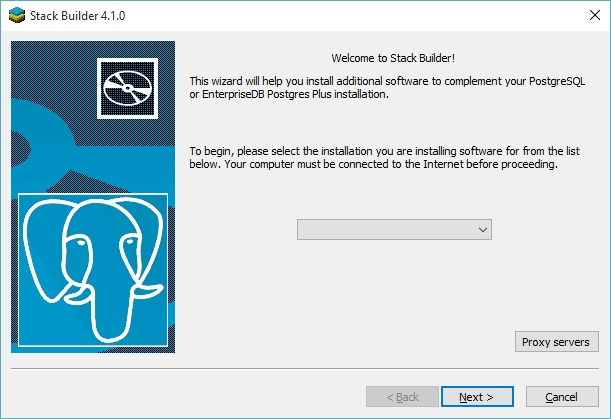
\includegraphics{./img/stack-builder-start.jpg}
  \caption{Application Stack Builder}
  \end{figure}
\item
  Pilih \textbf{PostgreSQL 10 (x64) on port 5432}, dan klik \textbf{Next \textgreater{}}. Jangan pilih yang \textbf{\textless{}remote server\textgreater{}} yaa\ldots{}, karena pilihan ini selanjutnya tidak menyediakan opsi instalasi Spatial Extensions (PostGIS dll.).

  \begin{figure}
  \centering
  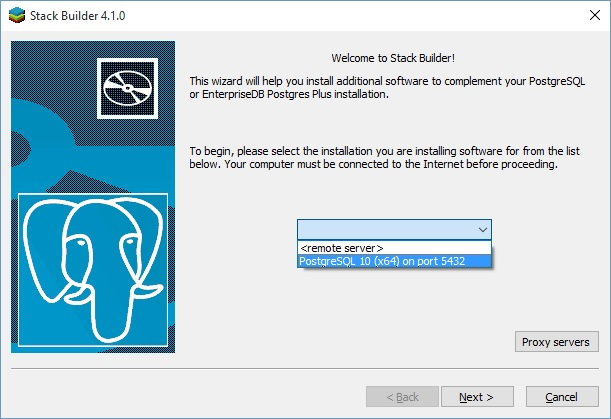
\includegraphics{./img/stack-builder-select-server.jpg}
  \caption{Application Stack Builder}
  \end{figure}

  Tunggu beberapa saat, Application Stack Builder akan men-\emph{download list} aplikasi yang bisa Anda \emph{install} di tahap selanjutnya. Jika sudah muncul tampilan:

  \begin{figure}
  \centering
  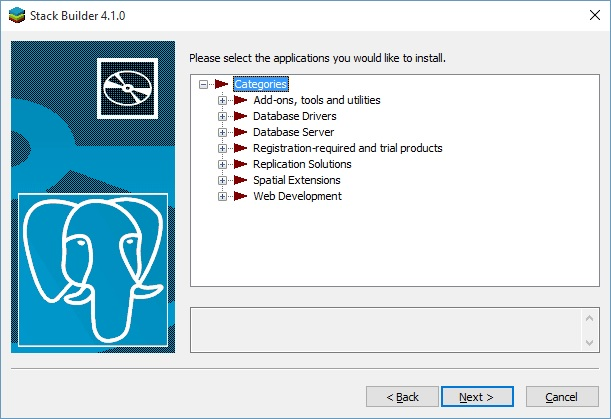
\includegraphics{./img/stack-builder-select-app.jpg}
  \caption{Application Stack Builder}
  \end{figure}
\item
  Pilih \textbf{Npgsql}, \textbf{pgJDBC} dan \textbf{psqlODBC} pada kelompok \textbf{Database Drivers}, dan \textbf{PostGIS 2.5 Bundle for PostgreSQL 10 (64 bit)} pada kelompok \textbf{Spatial Extensions}.

  \begin{figure}
  \centering
  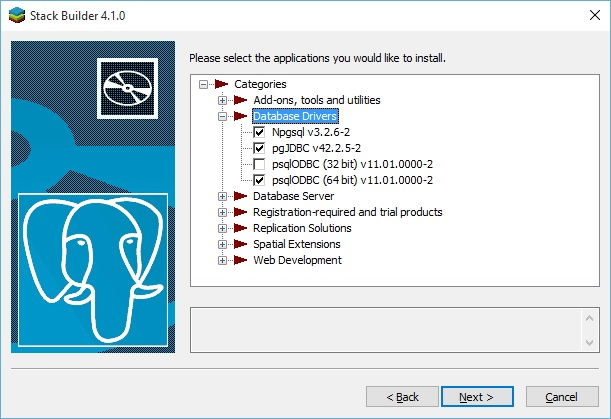
\includegraphics{./img/stack-builder-db-driver.jpg}
  \caption{Application Stack Builder}
  \end{figure}

  \begin{figure}
  \centering
  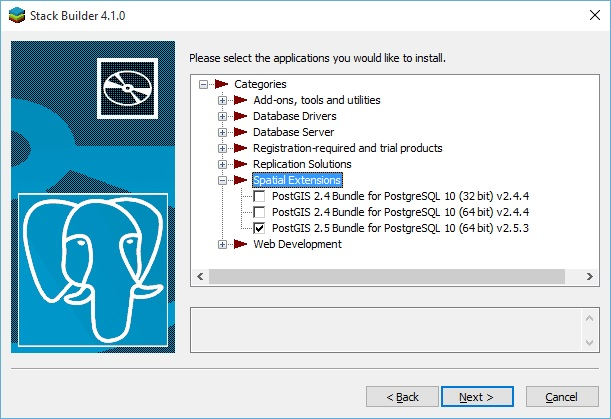
\includegraphics{./img/stack-builder-postgis.jpg}
  \caption{Application Stack Builder}
  \end{figure}

  Klik \textbf{Next \textgreater{}}, dan tunggu beberapa saat hingga Application Stack Builder selesai men-\emph{download} dan meng-\emph{install} seluruh aplikasi yang sudah dipilih. Setelah selesai, keluar/matikan Application Stack Builder-nya dan buka \emph{Start menu}.

  Pilih (atau cari dulu) menu \textbf{PostGIS 2.x Shapefile and DBF Loader Exporter}. Tampilan aplikasinya:

  \begin{figure}
  \centering
  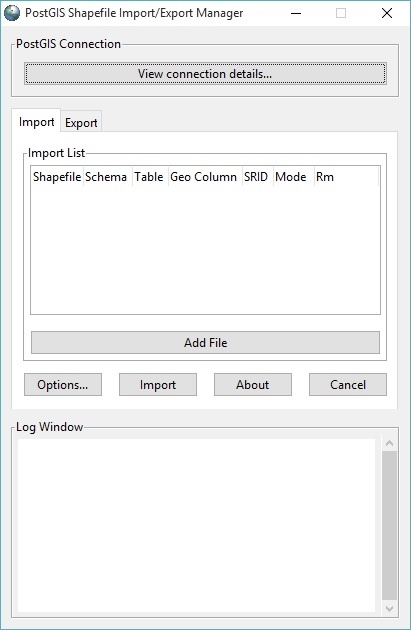
\includegraphics{./img/postgis-loader-start.jpg}
  \caption{PostGIS Shapefile DBF Loader}
  \end{figure}
\item
  \emph{Connection testing} ke server.

  Klik \textbf{View connection details\ldots{}}, dan isikan Username: \textbf{pgdbuser}, Password: {[}\emph{password}{]}, Server Host: \textbf{192.168.1.23} dan port-nya: \textbf{5432}, Database: \textbf{webmap\_db} seperti ini:

  \begin{figure}
  \centering
  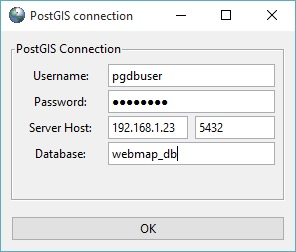
\includegraphics{./img/postgis-loader-connect-box.jpg}
  \caption{PostGIS Shapefile DBF Loader}
  \end{figure}

  Jika koneksinya sukses, maka pada bagian \textbf{Log Window} akan muncul log yang mengkonfirmasi bahwa koneksi berhasil.

  \begin{figure}
  \centering
  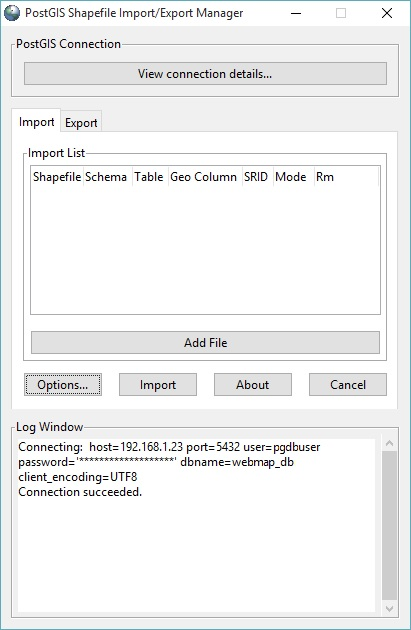
\includegraphics{./img/postgis-loader-connection-success.jpg}
  \caption{PostGIS Shapefile DBF Loader}
  \end{figure}

  Jika koneksi gagal, periksa kembali pengaturan koneksinya.

  Sekarang saatnya Anda mencoba meng-\emph{upload} sebuah shapefile ke PostgreSQL/PostGIS di server menggunakan \textbf{PostGIS 2.x Shapefile and DBF Loader Exporter}.

  O ya, tapi lebih baik kita bahas dulu spesifikasi file yang pada bagian 8.1 di atas saya sarankan untuk di-\emph{download}, yaitu \href{https://www.naturalearthdata.com/http//www.naturalearthdata.com/download/10m/cultural/ne_10m_admin_0_countries.zip}{\textbf{batas administrasi negara level 0}}. Kalau kita ekstrak file ini, maka kita akan memiliki 1 \emph{set files} yang yang nama file-nya identik, tapi \emph{extension}-nya berbeda. Dalam konteks pembahasan ini, kita hanya akan fokus pada file \texttt{ne\_10m\_admin\_0\_countries.prj} saja, karena pada saat \emph{upload} shapefile nanti, kita butuh informasi \textbf{SRID (Spatial Reference System Identifier)}.

  File ber-\emph{extension} \texttt{*.prj} ini berisi informasi tentang CRS (Coordinate Reference System) yang diterapkan/digunakan oleh file ber-\emph{extension} \texttt{*.shp} dan \texttt{*.shx} di direktori yang sama. Kalau Anda membuka file ini di ASCII text editor seperti Notepad atau Notepad++, dan Anda menemui \emph{entry} yang bertuliskan \textbf{WGS\_1984}, maka besar kemungkinan \textbf{SRID} -nya adalah \textbf{EPSG 4326}. Lebih lanjut lagi, ``tebakan'' SRID ini saya kira cukup masuk-akal karena shapefile ini \emph{coverage}-nya \emph{world}. Jika Anda ingin mengetahui lebih lanjut tentang CRS, WGS 1984, SRID, dan lain sebagainya yang terkait, silahkan gali lebih dalam, asal jangan ``tersesat'' saja (baca: menyerah, dan langsung ngikut paham bumi-datar. Hahaha\ldots{}).

  Kembali ke tampilan \textbf{PostGIS Shapefile and DBF Loader Exporter}, langsung saja klik \textbf{Add File}, maka dialog \textbf{Select a Shape file} muncul, pilih (klik) shapefile yang akan di-\emph{upload}, dan klik \textbf{Open}.

  \begin{figure}
  \centering
  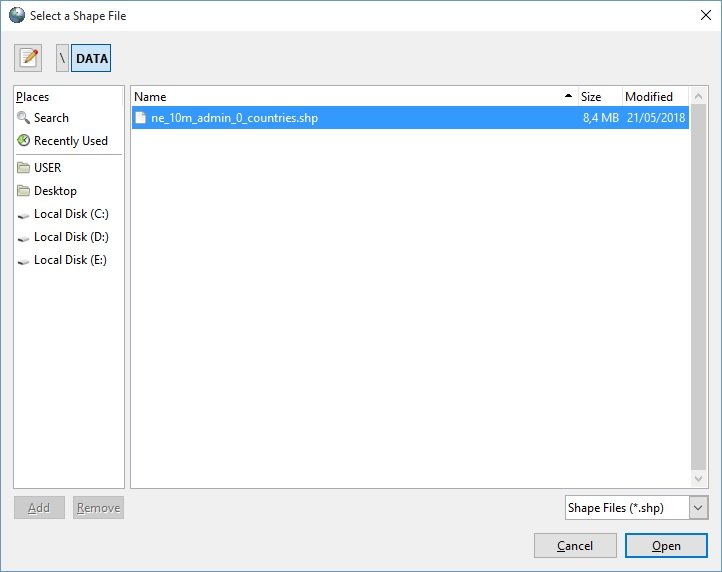
\includegraphics{./img/postgis-loader-select-shapefile-box.jpg}
  \caption{PostGIS Shapefile DBF Loader}
  \end{figure}

  Setelah klik \textbf{Open}, maka shapefile tersebut akan masuk ke \textbf{Import List}. Dalam tampilan ini mari kita fokus ke boks merah, yaitu kolom \textbf{SRID}.

  \begin{figure}
  \centering
  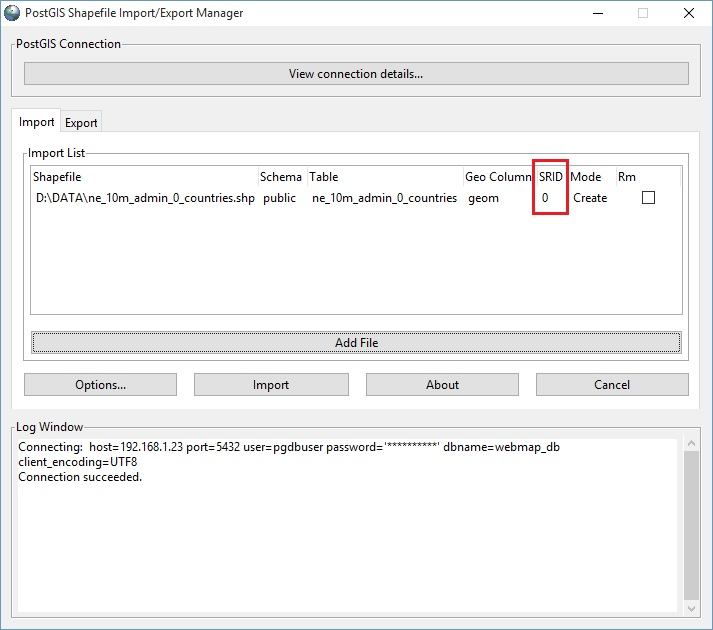
\includegraphics{./img/postgis-loader-srid-column.jpg}
  \caption{PostGIS Shapefile DBF Loader}
  \end{figure}

  Klik angka \textbf{0} dalam kolom, dan isi dengan angka \textbf{4326}, dan klik pada ruang kosong dalam \textbf{Import List}, di bawah \emph{entry} shapefile-nya. Untuk nama \textbf{Table} dan \textbf{Geo Column} yang akan jadi target di PostgreSQL/PostGIS biarkan saja apa-adanya.

  \begin{figure}
  \centering
  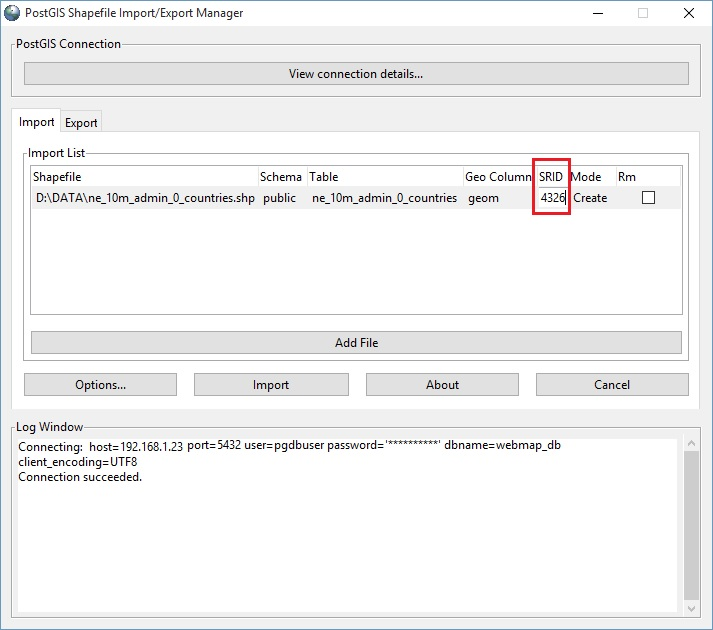
\includegraphics{./img/postgis-loader-4326.jpg}
  \caption{PostGIS Shapefile DBF Loader}
  \end{figure}

  Selanjutnya klik \textbf{Import}, dan tunggu beberapa saat sampai selesai. Jika tidak ada \emph{error} saat proses \emph{upload}, maka setelah selesai di \textbf{Log Window}-nya akan muncul konfirmasi bahwa \emph{upload} shapefile-nya berhasil.

  \begin{figure}
  \centering
  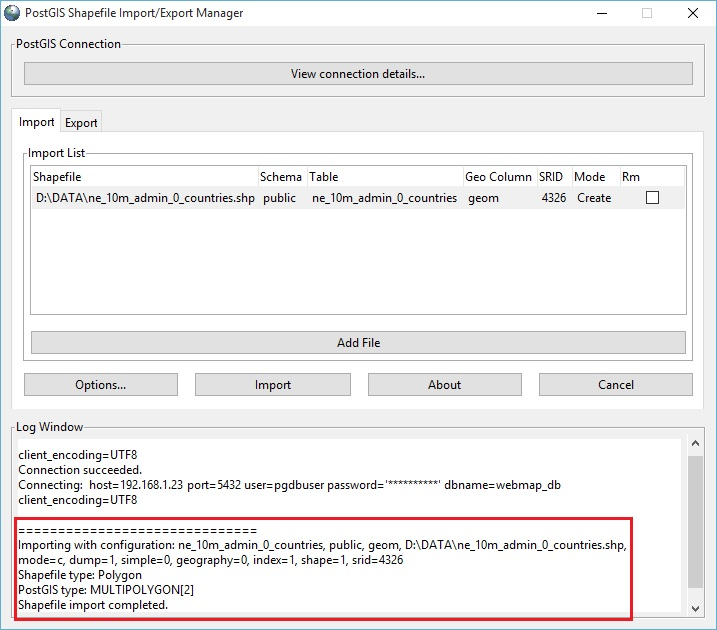
\includegraphics{./img/postgis-loader-import-completed.jpg}
  \caption{PostGIS Shapefile DBF Loader}
  \end{figure}

  Sampai pada tahap ini, di PostgreSQL/PostGIS server sudah ada contoh geodata yang sudah siap diakses dari berbagai kanal.
\item
  Testing PostGIS Layer di Quantum GIS.

  \emph{Test} mengakses PostGIS \emph{layer} yang paling sederhana adalah dengan menggunakan \textbf{Quantum GIS}. Aktifkan Quantum GIS Anda, buat \emph{project} baru, kemudian klik menu \textbf{Layer} -\textgreater{} \textbf{Data Source Manager}:

  \begin{figure}
  \centering
  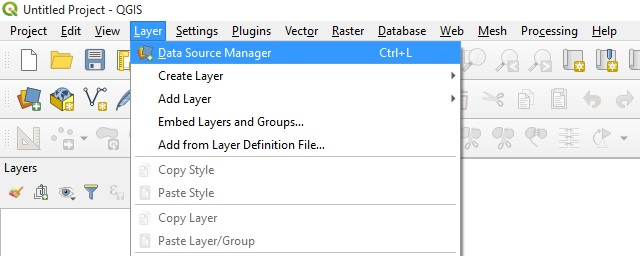
\includegraphics{./img/qgis-open-dsm.jpg}
  \caption{QGIS PostGIS Layer}
  \end{figure}

  Setelah dialog \textbf{Data Source Manager} muncul, klik \textbf{PostgreSQL} pada bagian kiri, sehingga muncul tampilan koneksi ke PostgreSQL di bagian kanan, dan pada bagian \textbf{Connections}, klik \textbf{New}:

  \begin{figure}
  \centering
  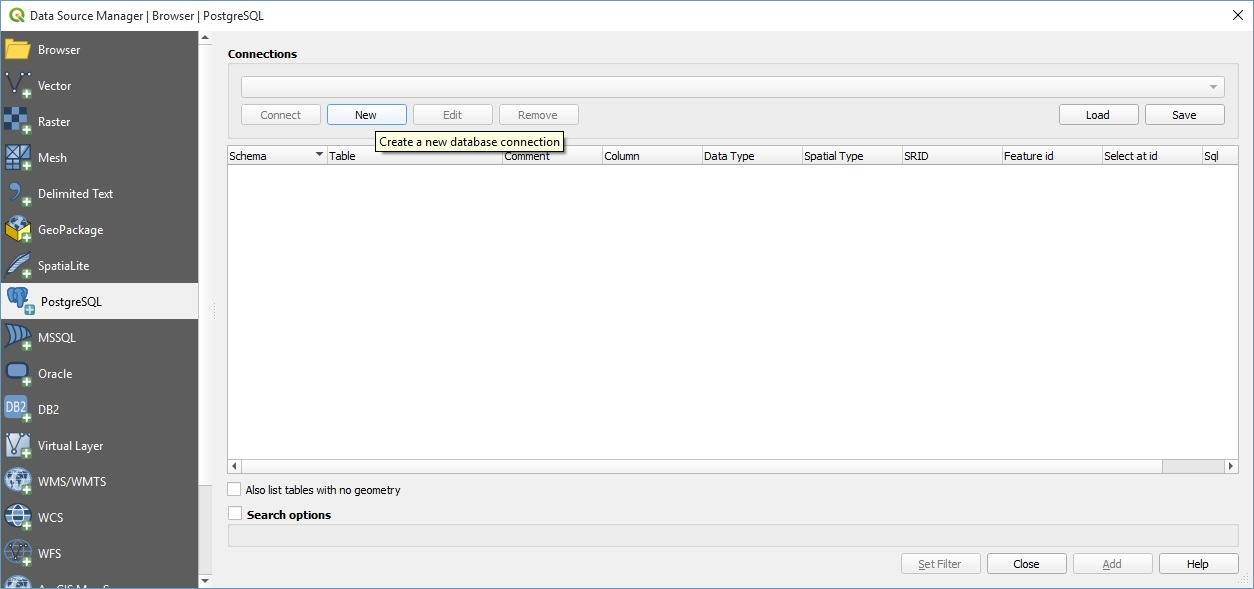
\includegraphics{./img/qgis-dsm-dialog.jpg}
  \caption{QGIS PostGIS Layer}
  \end{figure}

  Setelah Anda klik \textbf{New}, maka akan muncul dialog \textbf{Create a New PostGIS Connection}.

  \begin{figure}
  \centering
  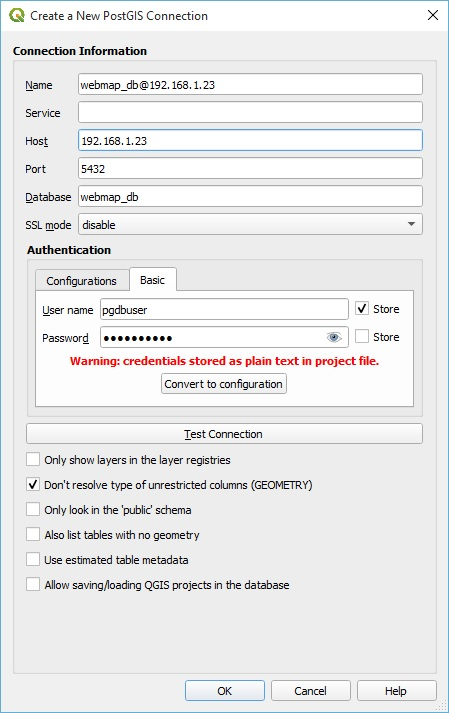
\includegraphics{./img/qgis-create-connection.jpg}
  \caption{QGIS PostGIS Layer}
  \end{figure}

  \begin{quote}
  Pada bagian \textbf{Connection Information}, isi Name: \textbf{\href{mailto:webmap_db@192.168.1.23}{\nolinkurl{webmap\_db@192.168.1.23}}} (atau yang lain sesuka Anda), \textbf{Service} dibiarkan kosong saja, Host: \textbf{192.168.1.23}, Port: \textbf{5432} dan Database: \textbf{webmap\_db}.
  \end{quote}

  \begin{quote}
  Pada bagian \textbf{Authentication}, klik \emph{tab} \textbf{Basic}, dan isi \textbf{User name}: \textbf{pgdbuser}, \emph{checkbox} \textbf{Store}-nya di-\emph{check}, \textbf{Password} diisi dengan \emph{password}-nya pgdbuser, dan \emph{checkbox} \textbf{Store}-nya dibiarkan \emph{unchecked} saja.
  \end{quote}

  \begin{quote}
  Berikutnya Anda bisa melakukan connection testing dengan meng-klik Test connection. Konfirmasi berhasil atau tidak-nya koneksi akan muncul pada bagian atas dialog box ini.
  \end{quote}

  \begin{quote}
  Jika Anda ingin hanya menampilkan \emph{table} yang memiliki \emph{geometry field} saja, \emph{check} saja \emph{checkbox} pada opsi \textbf{Don't resolve type of unrestricted columns (GEOMETRY)}.
  \end{quote}

  Setelah Anda klik \textbf{OK}, maka \emph{table} yang tadi sudah terbentuk saat kita meng-\emph{upload} shapefile akan muncul sebagai pilihan \emph{layer} yang akan ditampilkan.

  \begin{figure}
  \centering
  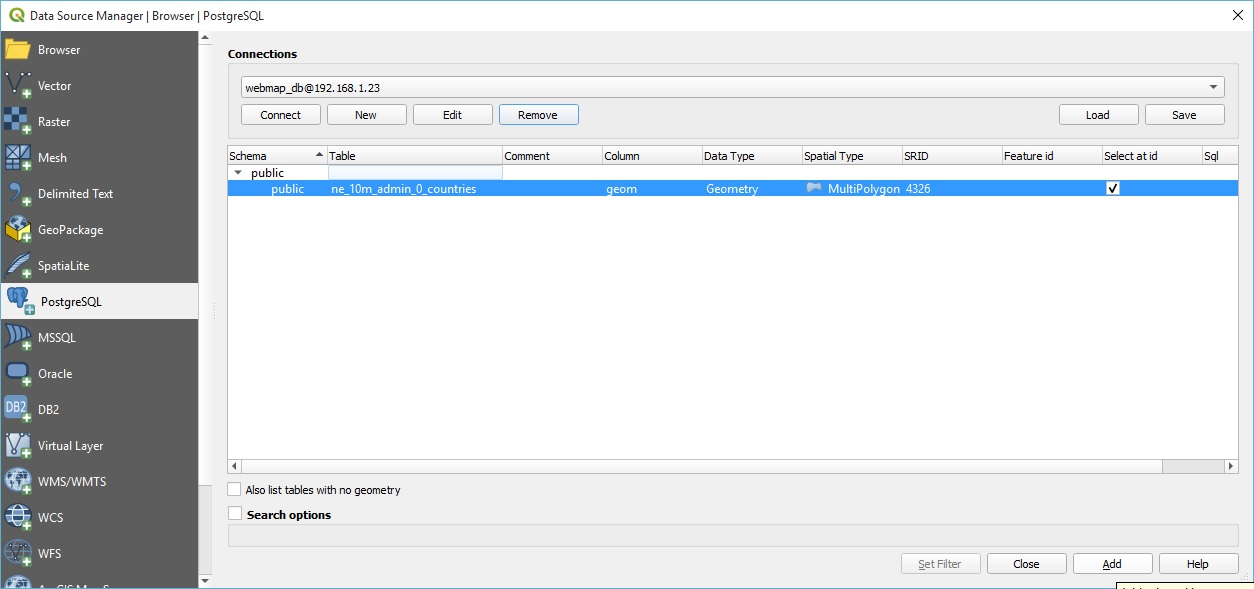
\includegraphics{./img/qgis-select-layers.jpg}
  \caption{QGIS PostGIS Layer}
  \end{figure}

  Klik (pilih) pada \emph{table} tersebut, kemudian klik \textbf{Add} pada bagian bawah dan tunggu sejenak hingga tampilan \emph{layer}-nya muncul di belakang dialog \textbf{Data Source Manager} ini. Selanjutnya klik \textbf{Close}.

  \begin{figure}
  \centering
  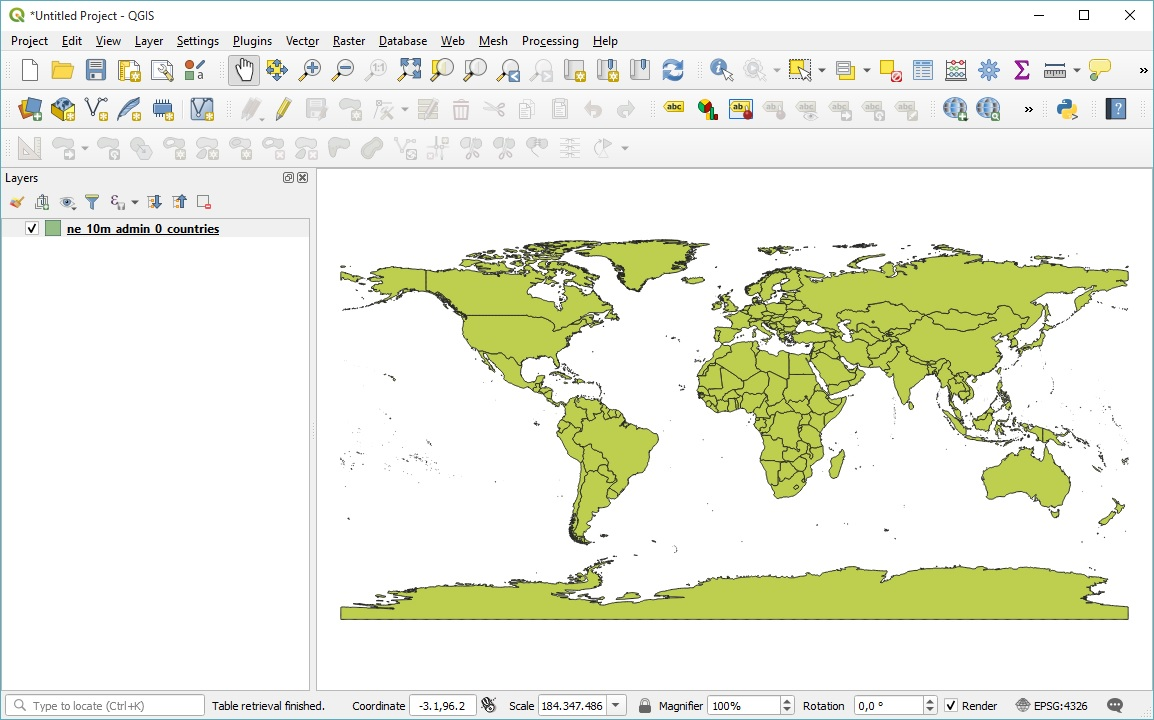
\includegraphics{./img/qgis-postgis-layer-loaded.jpg}
  \caption{QGIS PostGIS Layer}
  \end{figure}

  Jika \emph{layer} \textbf{ne\_10m\_admin\_0\_countries} sudah muncul, maka test PostGIS \emph{layer} Anda sudah berhasil.
\end{itemize}

\hypertarget{download-data}{%
\subsection{Download Data}\label{download-data}}

Service Kemendagri

\hypertarget{impor-data}{%
\subsection{Impor Data}\label{impor-data}}

\hypertarget{studi-kasus-pembangunan-basis-data-untuk-analisis-wilayah-layanan}{%
\chapter{Studi Kasus : Pembangunan Basis Data untuk Analisis Wilayah Layanan}\label{studi-kasus-pembangunan-basis-data-untuk-analisis-wilayah-layanan}}

\textbf{Topik}

\begin{itemize}
\tightlist
\item
  membuat desain basis data relasional menggunakan diagram ER
\item
  melakukan normalisasi dalam perancangan basis data
\item
  membangun basis data spasial untuk analisis wilayah layanan (\emph{\textbf{service area analyses}}) terkait fasiitas pendidikan dan kesehatan
\item
  melakukan integrasi data spasial dan non-spasial
\end{itemize}

\textbf{Perangkat}

\begin{itemize}
\tightlist
\item
  pgModeler

  \begin{itemize}
  \tightlist
  \item
    Download (\url{https://pgmodeler.io/download})
  \item
    Source code ~(\url{https://github.com/pgmodeler/pgmodeler.git})
  \end{itemize}
\item
  CASE tools (ArcGIS 10)
\end{itemize}

\textbf{Studi Kasus}

\begin{itemize}
\tightlist
\item
  Analisis Layanan Fasilitas Kesehatan
\end{itemize}

Data yang diperlukan :

\begin{verbatim}
1. Fasilitas 
  - Rumah Sakit
  - Rumah Bersalin
  - Posyandu
  - Puskesmas

2. Batas Administrasi

3. Jalan

4. Jumlah penduduk

5. Kepadatan penduduk (WorldPop)
\end{verbatim}

\begin{itemize}
\tightlist
\item
  Analisis Layanan Fasilitas Pendidikan (SMA)
\end{itemize}

Data yang diperlukan:

\begin{verbatim}
1. SMA

2. Batas Administrasi

3. Jalan

4. Jumlah penduduk

5. Kepadatan penduduk (WorldPop)
\end{verbatim}

\hypertarget{praktek-perancangan-basis-data}{%
\section{Praktek Perancangan Basis Data}\label{praktek-perancangan-basis-data}}

\textbf{Intisari}

\begin{enumerate}
\def\labelenumi{\arabic{enumi}.}
\item
  Melakukan identifikasi entitas
\item
  Melakukan identifikasi atribut untuk setiap entitas
\item
  Menggambarkan hubungan antara entitas
\item
  Melakukan normalisasi tabel
\end{enumerate}

\textbf{Sumber data}

Dapat dapat diperoleh dari :

\begin{itemize}
\item
  OpenStreetmap (\url{http://download.geofabrik.de/asia/indonesia.html})
\item
  Direktori Layanan ArcGIS Rest Service Kemendagri (\url{http://gis.dukcapil.kemendagri.go.id/arcgis/rest/services/})
\end{itemize}

\hypertarget{basis-data-lanjut}{%
\chapter{Basis Data Lanjut}\label{basis-data-lanjut}}

\textbf{Topik}

\hypertarget{non-spatial-sql-queries}{%
\section{Non-spatial SQL Queries}\label{non-spatial-sql-queries}}

\begin{enumerate}
\def\labelenumi{\arabic{enumi}.}
\tightlist
\item
  Membuat tabel baru
\end{enumerate}

Tujuan : Membuat tabel baru dari tabel yang sudah ada dengan kolom terpilih

\begin{verbatim}
CREATE TABLE kelurahan as SELECT geom, giskemen_2, giskemen_4, giskemen18,giskemen19,giskemen20,giskemen21, giskemen27, giskemen28 FROM public.desa_batam
\end{verbatim}

\begin{enumerate}
\def\labelenumi{\arabic{enumi}.}
\setcounter{enumi}{1}
\tightlist
\item
  Rename column
\end{enumerate}

Tujuan : Mengganti nama kolom tertentu

\begin{verbatim}
ALTER TABLE public.kelurahan RENAME COLUMN giskemen_2 TO nama_desa;
\end{verbatim}

\begin{enumerate}
\def\labelenumi{\arabic{enumi}.}
\setcounter{enumi}{2}
\tightlist
\item
  Mengubah Primary Key
\end{enumerate}

\begin{verbatim}
ALTER TABLE desa_batam DROP CONSTRAINT id;
\end{verbatim}

\begin{verbatim}
ALTER TABLE desa_batam RENAME COLUMN giskemen_4 TO id;
\end{verbatim}

\begin{verbatim}
ALTER TABLE desa_batam ADD PRIMARY KEY (id);
\end{verbatim}

\begin{enumerate}
\def\labelenumi{\arabic{enumi}.}
\setcounter{enumi}{3}
\tightlist
\item
  Menambah Kolom
\end{enumerate}

\begin{verbatim}
ALTER TABLE public.kelurahan ADD COLUMN giskemen33 FROM public.desa WHERE giskemen_4.public.desa.id = giskemen_4.public.kelurahan.id
\end{verbatim}

\hypertarget{spatial-sql-queries}{%
\section{Spatial SQL Queries}\label{spatial-sql-queries}}

\hypertarget{adjacent}{%
\subsection{Adjacent}\label{adjacent}}

\begin{enumerate}
\def\labelenumi{\arabic{enumi}.}
\tightlist
\item
  Create New Layer
\end{enumerate}

\begin{verbatim}
SELECT * into qlayer FROM kelurahan WHERE st_touches(kelurahan.geometry, ( SELECT geometry FROM kelurahan WHERE nama_desa = 'SADAI'))
\end{verbatim}

\begin{enumerate}
\def\labelenumi{\arabic{enumi}.}
\setcounter{enumi}{1}
\tightlist
\item
  Create As View
\end{enumerate}

\texttt{CREATE\ VIEW\ TestView\ AS\ \ SELECT\ *\ FROM\ kelurahan\ WHERE\ st\_touches(kelurahan.geom,\ (\ SELECT\ geom\ FROM\ kelurahan\ WHERE\ nama\_desa\ =\ \textquotesingle{}SADAI\textquotesingle{}));}

\hypertarget{backup-dan-restore}{%
\section{Backup dan Restore}\label{backup-dan-restore}}

\begin{itemize}
\item
  \textbf{Presentasi :}
  \href{https://gitpitch.com/firmanhadi/lapan-okt-19/master/}{https://gitpitch.com/firmanhadi/lapan-okt-19/master\#/}
\item
  \textbf{Video Proof of Concept}

  \begin{itemize}
  \tightlist
  \item
    Backup dengan pgBarman
  \end{itemize}

  \url{https://www.dropbox.com/s/tk2g296cc0pv6dh/backup_poc_v1.mkv?dl=0}

  \begin{itemize}
  \tightlist
  \item
    Pooling Mechanism
  \end{itemize}

  \url{https://www.dropbox.com/s/nl3xa2bnlay6ppk/pooling_mechanism_poc_v1.mkv?dl=0}

  \url{https://www.dropbox.com/s/dtugpqi6k8hcsc3/pooling_mechanism_poc_v2.mkv?dl=0}

  \begin{itemize}
  \tightlist
  \item
    Failover Mechanism
  \end{itemize}

  \url{https://www.dropbox.com/s/j5f9ks21db18ebv/replication_failover_poc_v1.mkv?dl=0}
\item
  \textbf{Software}

  \begin{itemize}
  \tightlist
  \item
    \url{https://sqlbackupandftp.com/postgresql-backup}
  \end{itemize}
\end{itemize}

\hypertarget{part-sistem-informasi-geografis}{%
\part{Sistem Informasi Geografis}\label{part-sistem-informasi-geografis}}

\hypertarget{pemodelan-sistem-informasi-geografis}{%
\chapter{Pemodelan Sistem Informasi Geografis}\label{pemodelan-sistem-informasi-geografis}}

\textbf{Referensi}

``Geographic Information System (GIS) modeling approach to determine the fastest delivery routes'': \url{https://www.sciencedirect.com/science/article/pii/S1319562X15001370}

\hypertarget{conceptual-framework}{%
\section{Conceptual framework}\label{conceptual-framework}}

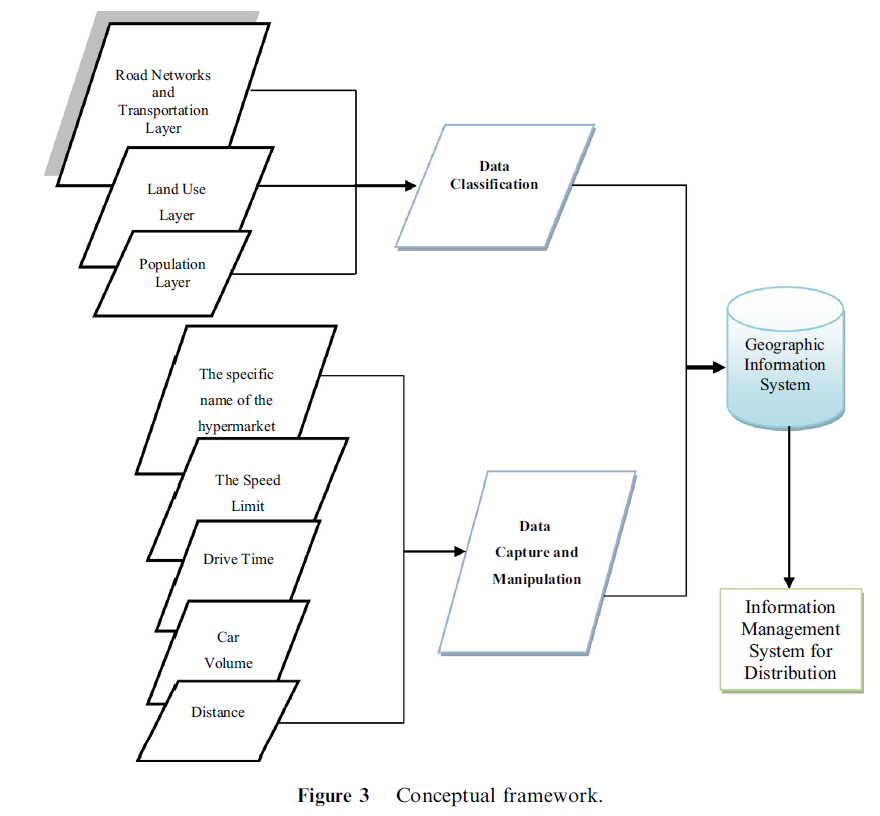
\includegraphics{./img/gismodel1.png}

\hypertarget{data}{%
\section{Data}\label{data}}

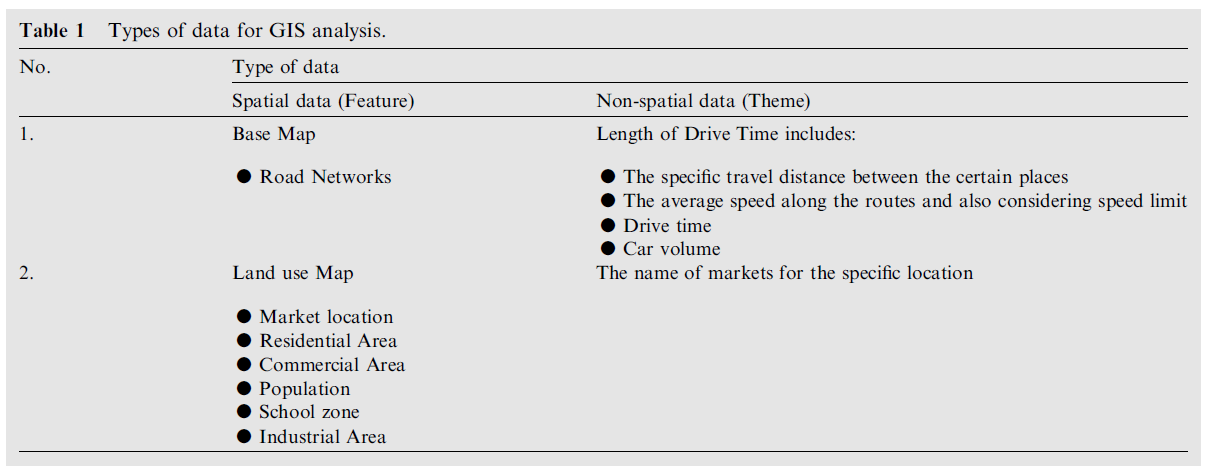
\includegraphics{./img/gismodel2.png}

\hypertarget{final-regression-model}{%
\section{Final regression model}\label{final-regression-model}}

LTIME = +0.2663 * CARVOLUME + 0.6984 * LLENGTH + 0.0203 * LPOP + 0.0605 * TWOWAY + 0.1681 * SCHOOL + 0.0317 * RESIDENTIAL - 0.5497

\hypertarget{studi-kasus-pemodelan-sig}{%
\section{Studi Kasus : Pemodelan SIG}\label{studi-kasus-pemodelan-sig}}

\hypertarget{analisis-wilayah-layanan-service-area-analyses}{%
\subsection{Analisis Wilayah Layanan (Service Area Analyses)}\label{analisis-wilayah-layanan-service-area-analyses}}

\begin{enumerate}
\def\labelenumi{\arabic{enumi}.}
\item
  Load layer jalan dan fasilitas kesehatan dalam format UTM (Zona 48N).
\item
  Load raster kepadatan penduduk
\item
  Melakukan analisis \textbf{\emph{service area}}
\end{enumerate}

\begin{itemize}
\tightlist
\item
  Processing \textgreater{} Network analyses \textgreater{} Service area
\end{itemize}

\begin{enumerate}
\def\labelenumi{\arabic{enumi}.}
\setcounter{enumi}{3}
\item
  Create buffer from service area lines
\item
  Calculate raster using vector
\end{enumerate}

\begin{itemize}
\tightlist
\item
  Zonal statistics
\end{itemize}

\hypertarget{menghitung-jumlah-rumah-di-sempadan-sungai}{%
\subsection{Menghitung jumlah rumah di sempadan sungai}\label{menghitung-jumlah-rumah-di-sempadan-sungai}}

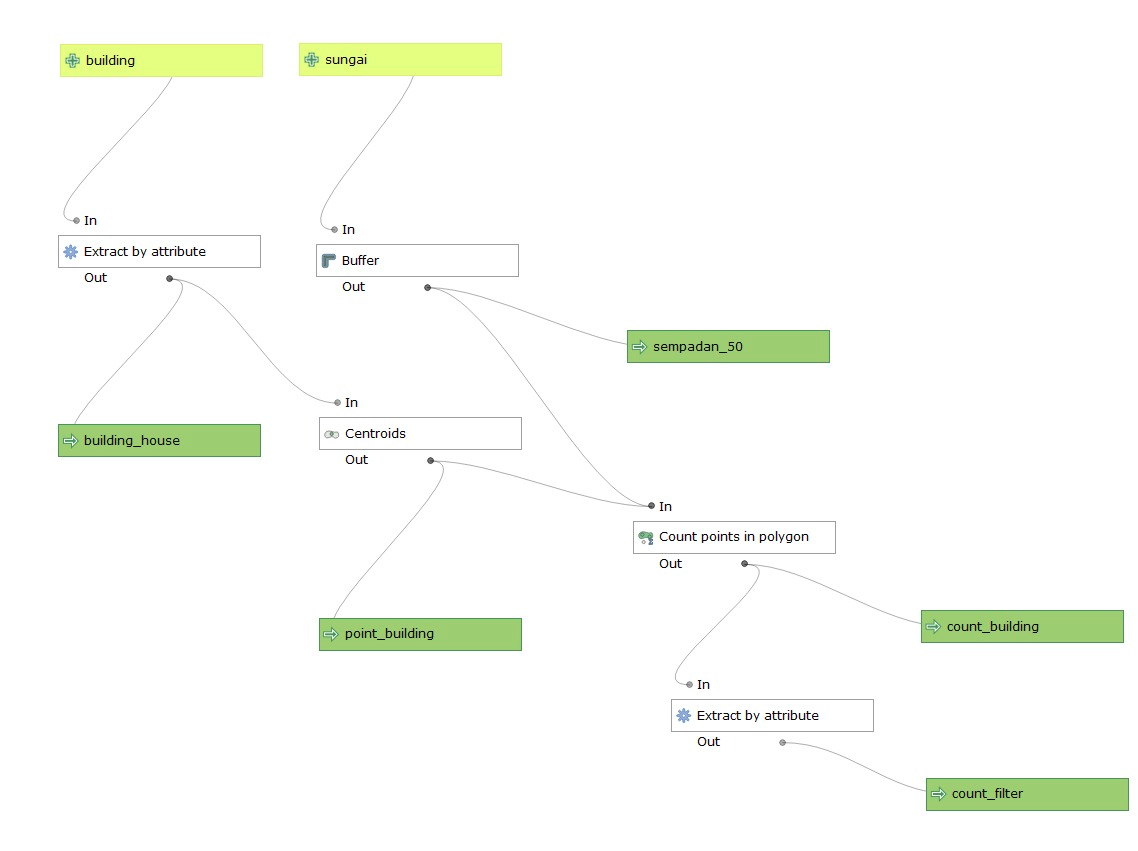
\includegraphics{./img/gismodel4.png}

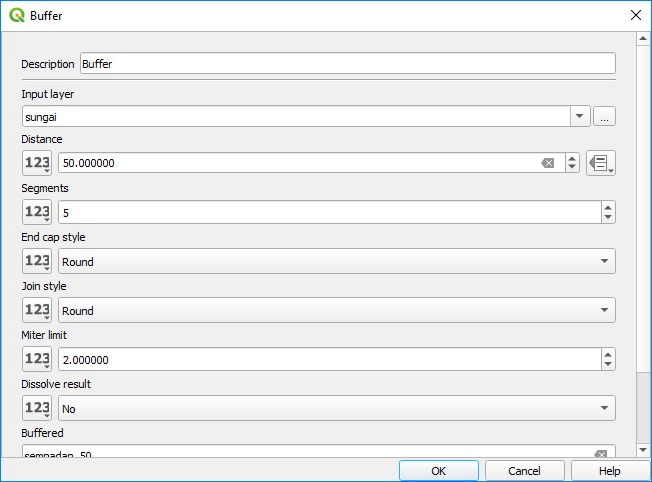
\includegraphics{./img/gismodel6.png}

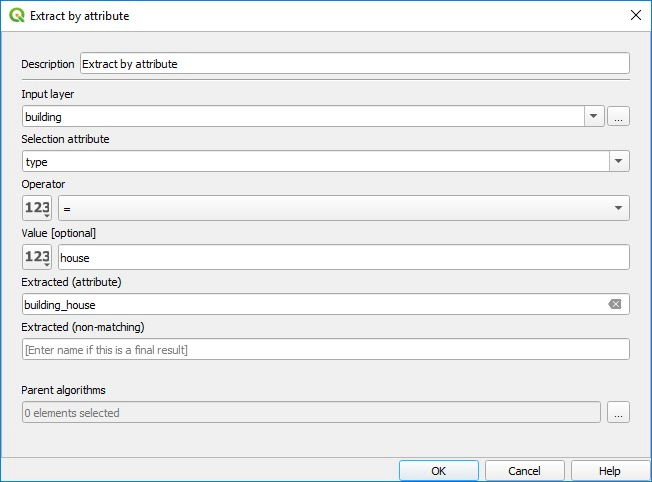
\includegraphics{./img/gismodel7.png}

\hypertarget{hari_keenam}{%
\chapter{Analisis Sistem Informasi Geografis}\label{hari_keenam}}

\textbf{Data}

Data dapat diunduh di tautan berikut \url{https://firmanhadi.github.io/training-for-gis-analyses/img/Day6.zip}

Analisis spasial adalah sebuah proses untuk mengkaji lokasi, atribut dan hubungan antara fitur dari data spasial melalui cara overlay dan teknik analisis lainnya, dalam rangka menjawab pertanyaan atau mendapatkan pemahaman yang bermanfaat. Analisis spasial mengekstrak atau membuat informasi baru dari data spasial.

\hypertarget{basic-geoprocessing}{%
\section{Basic Geoprocessing}\label{basic-geoprocessing}}

Geoprocessing adalah operasi SIG untuk memanipulasi data. Operasi geoprocessing membutuhkan input, melakukan operasi tertentu pada data tersebut dan memberikan hasil dari operasi dalam bentuk output dataset, seringkali disebut juga data turunan.

Operasi geoprocessing yang umum adalah overlay, feature selection dan analisis, pemrosesan topologi dan konversi data. Geoprocessing memungkinkan Anda untuk mendefinisikan, mengelola dan menganalisis informasi geografis yang digunakan untuk membuat keputusan.

Dengan kata lain, ektraksi atau pengubahan informasi seperti yang Anda harapkan dari data selalu melibatkan geoprocessing.

\hypertarget{penapisan-data}{%
\subsection{Penapisan data}\label{penapisan-data}}

Kawasan lindung (taman nasional, suaga margasatwa dan hutan lindung) direncanakan dan dikelola dengan tujuan utama untuk konservasi biodiversitas. Hampir semua kawasan lindung terpapar interaksi dengan manusia, baik di dalam ataupun di luar kawasan. Hal ini akan berpengaruh terhadap hidupan liar dan habitatnya. Oleh karena itu, pertumbuhan populasi merupakan salah satu masalah utama dalam pengelolaan kawasan lindung. Hal tersebut akan memicu perubahan tutupan lahan dan penggunaan lahan, yang berdampak pada semakin tingginya tekanan terhadap kawasan lindung.

Walaupun efek kawasan lindung terhadap permukiman manusia masih menjadi perdebatan, ada sebuah kebutuhan pengelolaan interaksi tersebut, baik dalam hal positif ataupun negatif, yang menjadi vital dalam menjaga kelestarian layanan ekosistem. Dengan alasan ini, memetakan sebaran permukiman adalah salah hal yang dilakukan pertama kali dalam mengelola kawasan lindung.

Dalam pelatihan ini, permukiman direpresentasikan sebagai titik perkampungan dari OpenStreetMap yang akan diekstrak melalui query atau penapisan data. Caranya adalah sebagai berikut :

\begin{enumerate}
\def\labelenumi{\arabic{enumi}.}
\item
  Buka osm\_points.shp
\item
  Klik-kanan pada Layer dan pilih Open Attribute Table.
\end{enumerate}

\begin{figure}

{\centering 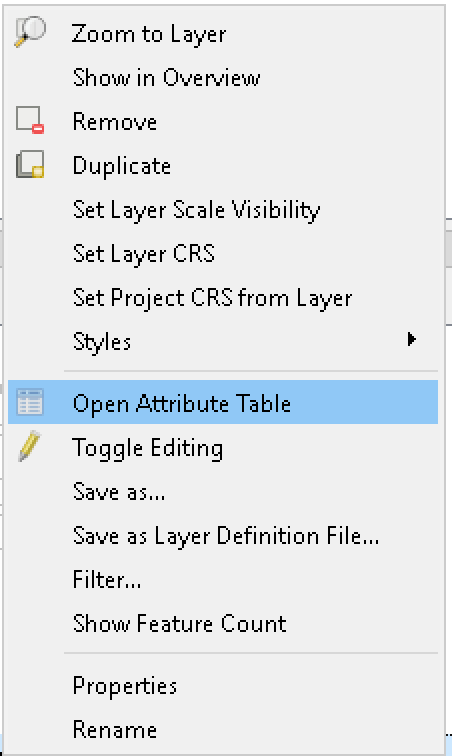
\includegraphics[width=0.3\linewidth]{images/04/fig24} 

}

\caption{Open Attribute Table}\label{fig:fig1424}
\end{figure}

\begin{enumerate}
\def\labelenumi{\arabic{enumi}.}
\setcounter{enumi}{2}
\tightlist
\item
  Klik tombol \textbf{Select features by expression}.
\end{enumerate}

\begin{figure}

{\centering 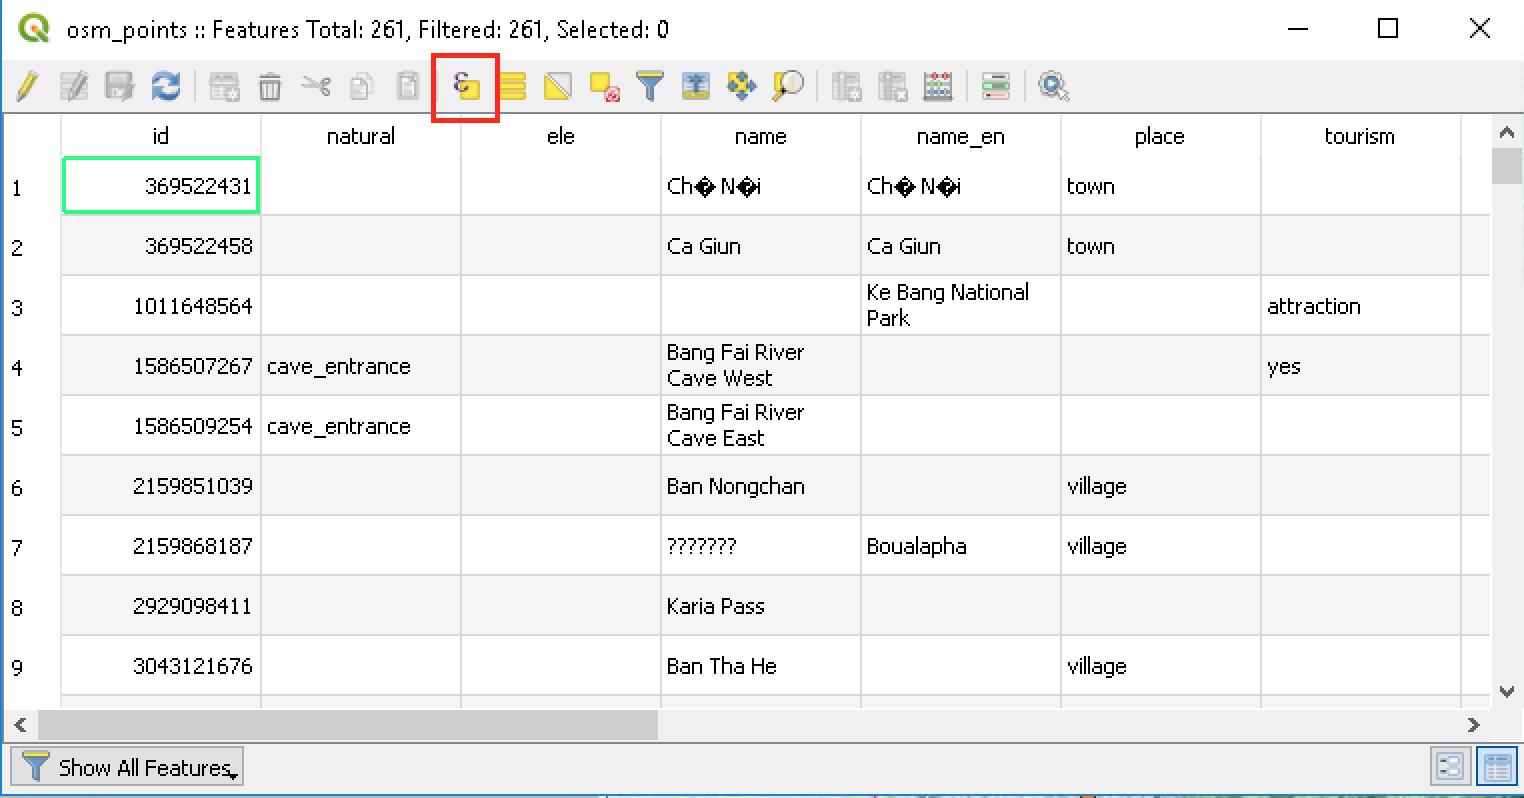
\includegraphics[width=0.7\linewidth]{images/04/fig25} 

}

\caption{Select Features by expression button}\label{fig:fig1425}
\end{figure}

\begin{enumerate}
\def\labelenumi{\arabic{enumi}.}
\setcounter{enumi}{3}
\tightlist
\item
  Pilih \textbf{place} untuk opsi \textbf{Field and Values}. Klik tombol \textbf{All unique} untuk melihat nilai yang ada di kolmo Place. Ketik ekspresi ``place'' = `village', klik tombol \textbf{Select features} di bagian bawah untuk melakukan penapisan data.
\end{enumerate}

\begin{figure}

{\centering 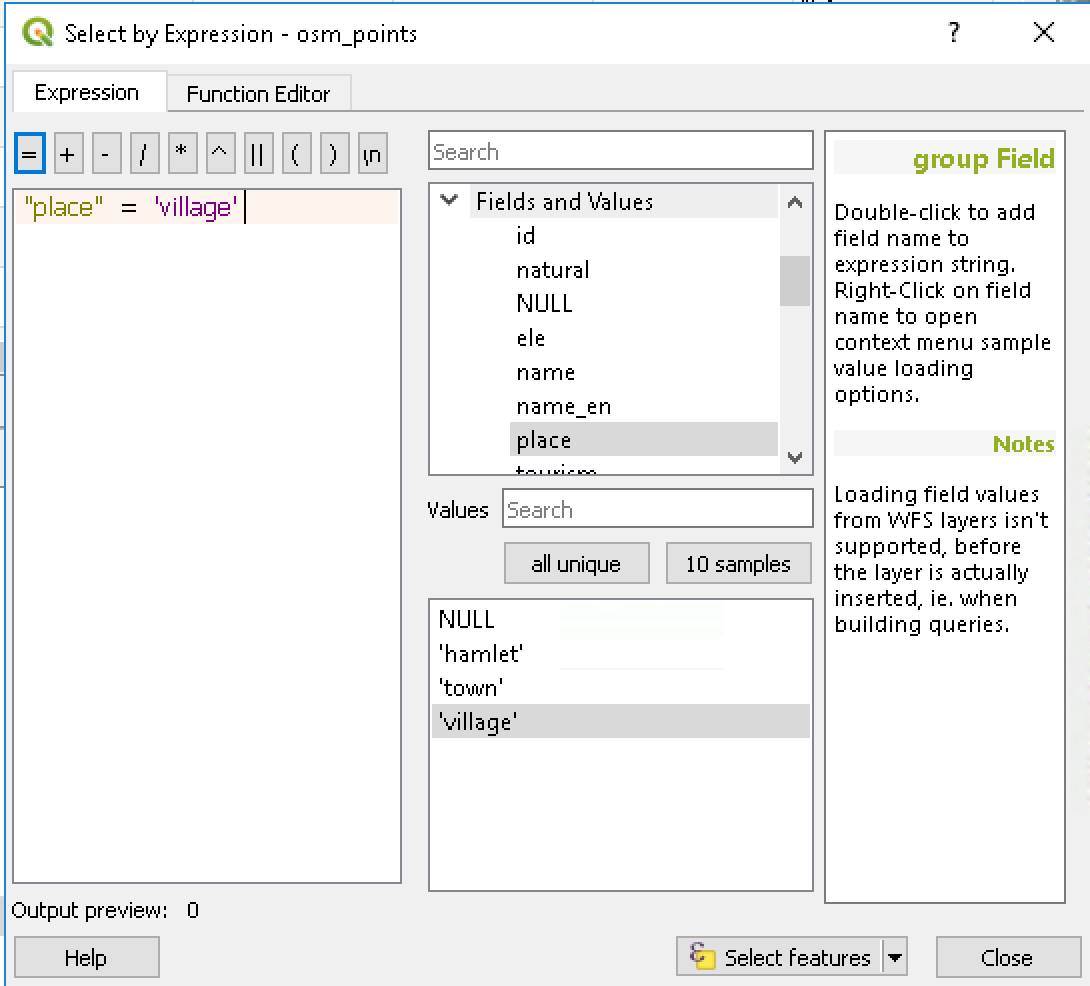
\includegraphics[width=0.7\linewidth]{images/04/fig26} 

}

\caption{Select by expression window}\label{fig:fig1426}
\end{figure}

\begin{enumerate}
\def\labelenumi{\arabic{enumi}.}
\setcounter{enumi}{4}
\tightlist
\item
  Baris yang terpilih akan berwarna biru (highlight).
\end{enumerate}

\begin{figure}

{\centering \includegraphics[width=0.7\linewidth]{images/04/fig27} 

}

\caption{Selected records}\label{fig:fig1427}
\end{figure}

\begin{enumerate}
\def\labelenumi{\arabic{enumi}.}
\setcounter{enumi}{4}
\item
  Klik kanan pada Layer \textbf{osm\_points} layer dan pilih \textbf{``Save as''}
\item
  Isikan pilihan seperti pada Gambar \ref{fig:fig1428}. Dan jangan lupa untuk memilih \textbf{Save only selected features}.
\end{enumerate}

Untuk mengubah Coordinate Reference System (CRS), klik ikon Globe pada opsi CRS dan ketikkan 32648 dalam kotak Filter.

\begin{figure}

{\centering \includegraphics[width=0.7\linewidth]{images/04/fig29} 

}

\caption{Save Vector Layer As window}\label{fig:fig1429}
\end{figure}

\begin{figure}

{\centering \includegraphics[width=0.7\linewidth]{images/04/fig28} 

}

\caption{Selecting new CRS}\label{fig:fig1428}
\end{figure}

\hypertarget{dissolve}{%
\subsection{Dissolve}\label{dissolve}}

Satu atau lebih atribut dapat dipilih untuk menggabungkan (merge) geometri yang termasuk ke dalam kelas yang sama, atau semua geometri, dapat digabungkan.

Semua luaran (output) geometri akan dikonversi ke dalam bentuk multi geometri. Apabila inputnya adalah Layer poligon, common boundaries (batas bersama) dari poligon-poligon tetangga yang digabungkan, akan dihapus.

Untuk latihan ini, data yang akan digunakan adalah batas administrasi Laos. Batas ini terdiri dari tiga level (1) negara, (2) propinsi dan (3) distrik. Kita akan menggabungkan batas distrik ke tingkat propinsi.

Silakan ikuti langkah berikut untuk menggabungkan poligon berdasarkan atribut:

\begin{enumerate}
\def\labelenumi{\arabic{enumi}.}
\tightlist
\item
  Buka gadm36\_LAO\_2.shp di Map Display.
\end{enumerate}

\begin{figure}

{\centering \includegraphics[width=0.7\linewidth]{images/04/fig19} 

}

\caption{Lao Admin Boundary Level 2}\label{fig:fig1419}
\end{figure}

\begin{enumerate}
\def\labelenumi{\arabic{enumi}.}
\setcounter{enumi}{1}
\tightlist
\item
  Pilih \textbf{\emph{Vector -\textgreater{} GeoProcessing Tools -\textgreater{} Dissolve}}
\end{enumerate}

\begin{figure}

{\centering \includegraphics[width=0.6\linewidth]{images/04/fig19a} 

}

\caption{Dissolve menu}\label{fig:fig1419a}
\end{figure}

\begin{enumerate}
\def\labelenumi{\arabic{enumi}.}
\setcounter{enumi}{2}
\tightlist
\item
  Klik \ldots{} pada \textbf{Unique ID Field}, pilih \textbf{NAME1} dan klik OK.
\end{enumerate}

\begin{figure}

{\centering \includegraphics[width=0.6\linewidth]{images/04/fig20} 

}

\caption{NAME1 selected as Unique ID}\label{fig:fig1420}
\end{figure}

\begin{enumerate}
\def\labelenumi{\arabic{enumi}.}
\setcounter{enumi}{3}
\tightlist
\item
  Pada menu Dissolve, klik \textbf{Run in the background} untuk menjalankan proses.Hasilnya akan ditampilkan di Map Display.
\end{enumerate}

\begin{figure}

{\centering \includegraphics[width=0.7\linewidth]{images/04/fig21} 

}

\caption{Dissolved region}\label{fig:fig1421}
\end{figure}

\hypertarget{polygon-dari-layer-extent}{%
\subsection{Polygon dari layer extent}\label{polygon-dari-layer-extent}}

Fungsi ini bermanfaat ketika kita ingin memotong raster atau vektor dengan menggunakan extent (bounding box) dari fitur tertentu.

Ikuti langkah berikut untuk melakukan ekstraksi batas dari poligon:

\begin{enumerate}
\def\labelenumi{\arabic{enumi}.}
\item
  Pilih \textbf{Vector -\textgreater{} Research Tools -\textgreater{} Extract layer extent}
\item
  Anda dapat mengatur apakah luaran disimpan sebagai layer sementara atau disimpan ke dalam berkas baru.
\end{enumerate}

\begin{figure}

{\centering \includegraphics[width=0.7\linewidth]{images/04/fig22} 

}

\caption{Extract layer extent}\label{fig:fig1422}
\end{figure}

\begin{enumerate}
\def\labelenumi{\arabic{enumi}.}
\setcounter{enumi}{2}
\tightlist
\item
  Hasil dari proses ini adalah sebuah poligon kotak (persegi panjang) berdasarkan batas koordinat kiri-atas dan kanan-bawah dari fitur yang digunakan.
\end{enumerate}

\begin{figure}

{\centering \includegraphics[width=0.7\linewidth]{images/04/fig23} 

}

\caption{Layer extent created}\label{fig:fig1423}
\end{figure}

\hypertarget{reklasifikasi}{%
\subsection{Reklasifikasi}\label{reklasifikasi}}

Fitur ini merupakan salah satu teknik yang bermanfaat untuk mengubah rentang nilai atau mengelompokkannya ke dalam kategori yang baru.

Kita akan melakukan klasifikasi ketinggian ke dalam tiga kelas:

\begin{verbatim}
- Kurang dari 1.000 m

- Antara 1.000 dan 2.000 m

- Lebih dari 2.000 m
\end{verbatim}

Untuk melakukan ini, silakan ikuti tahapan berikut :

\begin{enumerate}
\def\labelenumi{\arabic{enumi}.}
\item
  Buka \textbf{srtm\_58\_09.tif}
\item
  Buka fungsi \textbf{r.reclass} dari menu \textbf{Processing Toolbox}. Isi pilihan seperti terlihat dalam gambar dan klik \textbf{Run}.
\end{enumerate}

\begin{figure}

{\centering \includegraphics[width=0.7\linewidth]{images/04/fig74} 

}

\caption{Reclassifying the elevation data}\label{fig:fig1474}
\end{figure}

\begin{enumerate}
\def\labelenumi{\arabic{enumi}.}
\setcounter{enumi}{2}
\tightlist
\item
  Hasilnya adalah layer dengan kelas baru
\end{enumerate}

\begin{figure}

{\centering \includegraphics[width=0.7\linewidth]{images/04/fig75} 

}

\caption{Reclassified elevation data}\label{fig:fig1475}
\end{figure}

Nilai dari setiap piksel dibandingkan dengan rentang limit yang ada di lookup table.
Apabila nilai piksel termasuk ke dalam kelas tertentu, nilai kelas untuk rentang ini akan digunakan di dalam layer luaran.

\hypertarget{terrain-analyses}{%
\section{Terrain analyses}\label{terrain-analyses}}

Tipe raster tertentu memungkinkan Anda untuk mendapatkan informasi yang lebih terkait terrain. Biasanya Digital Elevation Models (DEMs) digunakan untuk keperluan ini.

\hypertarget{persiapan}{%
\subsection{Persiapan}\label{persiapan}}

\begin{enumerate}
\def\labelenumi{\arabic{enumi}.}
\item
  Buka \textbf{srtm\_58\_09.tif} (ada di dalam sub folder TIF). Layer ini merupakan DEM dengan
  EPSG:4326 CRS dan ketinggian dalam kaki (feet). Karakteristik ini tidak cocok untuk algoritma terrain analyses, harus dikonversi terlebih dahulu ke dalam proyeksi meter (Universal Transverse Mercator).
\item
  Reproyeksi layer ke sistem CRS EPSG:32648, menggunakan pilihan \textbf{Save as\ldots{}} pada menu yang muncul ketika di-klik kanan pada nama layer.
\item
  Buka layer yang dihasilkan.
\end{enumerate}

Ada hal yang perlu diperhatikan ketika menerapkan algoritma terrain analyses, agar hasilnya benar.

Salah satu permasalahan utamanya adalah apabila raster yang digunakan memiliki piksel dengan ukuran panjang dan lebar yang tidak sama (bukan bujur sangkar). Asumsi yang biasa digunakan adalah semua piksel pasti bujur sangkar. Namun seringkali data yang kita dapatkan tidak seperti itu.

Oleh karena itu, tahapan yang perlu dilakukan adalah mengekspor layer dan mendefinisikan ukuran piksel dengan nilai yang sama, misalnya 30 atau 90 m. Caranya adalah dengan klik kanan pada nama layer dan pilih \textbf{Save as \ldots{} }. Pada dialog \textbf{\emph{save}} yang ada, pastikan untuk mengisikan nilai piksel di bagian bawah dialog :

\begin{figure}

{\centering \includegraphics[width=0.7\linewidth]{images/04/fig71} 

}

\caption{Save raster layer as}\label{fig:fig1471}
\end{figure}

\hypertarget{kelerengan}{%
\subsection{Kelerengan}\label{kelerengan}}

Kelerengan (\textbf{Slope}) merupakan salah satu parameter dasar yang dapat diturunkan dari DEM.
Ia adalah turunan pertama dari DEM dan menggambarkan laju perubahan ketinggian. \textbf{Slope} dihitung dengan melakukan analisis ketinggian dari setiap piksel, membandingkannya dengan ketinggian piksel di sekelilingnya. Untuk menghitungnya di QGIS, silakan ikuti cara berikut :

\begin{enumerate}
\def\labelenumi{\arabic{enumi}.}
\tightlist
\item
  Pada opsi \textbf{Processing Toolbox} , pilih algoritma \textbf{Slope}, klik ganda untuk membukanya.
\end{enumerate}

\begin{figure}

{\centering \includegraphics[width=0.7\linewidth]{images/04/fig72} 

}

\caption{Calculating slope}\label{fig:fig1472}
\end{figure}

\begin{enumerate}
\def\labelenumi{\arabic{enumi}.}
\setcounter{enumi}{1}
\item
  Pilih \textbf{DEM} sebagai layer masukan (input).
\item
  Klik \textbf{Run} untuk menjalankan prosesnya.
\end{enumerate}

\hypertarget{hillshade}{%
\subsection{Hillshade}\label{hillshade}}

Layer \textbf{hillshade} umumnya digunakan untuk memperbagus tampilan peta dan topografi yang intuitif, dengan mensimulasikan sumber cahaya dan bayangan yang dibentuk oleh permukaan bumi. \textbf{Hillshade} dapat dihitung dengan cara sebagai berikut :

\begin{enumerate}
\def\labelenumi{\arabic{enumi}.}
\tightlist
\item
  Pada opsi \textbf{Processing Toolbox}, cari algoritma \textbf{Hillshade} dan klik-ganda untuk membuka menunya.
\end{enumerate}

\begin{figure}

{\centering \includegraphics[width=0.7\linewidth]{images/04/fig73} 

}

\caption{Calculating hillshade}\label{fig:fig1473}
\end{figure}

\begin{enumerate}
\def\labelenumi{\arabic{enumi}.}
\setcounter{enumi}{1}
\item
  Pilih DEM sebagai \textbf{Input layer}, gunakan parameter default.
\item
  Klik \textbf{Run} untuk menjalankan algoritmanya.
\end{enumerate}

\hypertarget{density-analyses-analisis-kepadatan}{%
\section{Density Analyses (Analisis Kepadatan)}\label{density-analyses-analisis-kepadatan}}

Seringkali kita harus bekerja dengan data besar dan padat fiturnya, yang membuat penampilan datanya lambat. Jumlahnya yang ribuan atau bahkan jutaan fitur seringkali sulit diinterpretasi, terjadi overlap antar fitur yang menyebabkan pendeteksian pola cluster atau distribusinya tidak mudah untuk dilakukan.

Pada bagian ini, kita akan belajar mengenai teknik yang memungkinkan visualisasi dataset semacam itu dengan bentuk yang lebih mudah dibaca dan dengan waktu pemuatan (\textbf{loading}) yang lebih cepat. Setelah melakukan praktek di bagian ini, Anda diharapkan mampu melakukan analisis kepadatan (\textbf{density analyses}) untuk data yang Anda miliki dan mengekstrak informasi dari peta kepadatan.

\hypertarget{konsep}{%
\subsection{Konsep}\label{konsep}}

Peta kepadatan memungkinkan estimasi visual konsentrasi objek atau peristiwa di area studi. Peta seperti itu sangat berguna untuk penilaian pola distribusi fitur di wilayah studi. Ketika kita cukup menambahkan lokasi fitur atau peristiwa (misalnya, sebagai titik) ke peta, kita tidak dapat melihat perubahan konsentrasi mereka di area yang berbeda. Analisis kepadatan memberi kita fungsionalitas seperti itu dengan menggunakan karakteristik area yang seragam, seperti jumlah fitur per hektar atau kilometer persegi.

Peta kepadatan memberi kita kemampuan untuk memperkirakan konsentrasi beberapa fitur dalam suatu area. Ini membantu kita menemukan area di mana reaksi mendesak diperlukan atau yang cocok dengan kriteria. \textbf{Heatmap} juga membantu mengontrol kondisi dan perubahannya.

Peta kepadatan juga sangat berguna ketika wilayah yang dipetakan (misalnya, kabupaten) memiliki ukuran yang berbeda. Misalnya, jika kita ingin tahu berapa banyak orang yang tinggal di setiap kabupaten, kita hanya perlu peta ordinal dengan data populasi. Menurut peta ini, sebuah distrik besar mungkin memiliki populasi yang lebih tinggi daripada distrik yang lebih kecil. Tetapi jika kita ingin mengidentifikasi kabupaten dengan konsentrasi populasi yang lebih tinggi, maka kita membutuhkan peta kepadatan untuk melihat jumlah orang per kilometer persegi. Dan peta kepadatan akan menunjukkan kepada kita bahwa, pada kenyataannya, daerah kecil dengan kepadatan penduduk yang tinggi mungkin memiliki lebih banyak orang per kilometer persegi daripada kabupaten yang lebih besar.

Secara umum, kita dapat menunjukkan pada peta distribusi kepadatan fitur itu sendiri (misalnya, sekolah), serta distribusi beberapa karakteristik numerik fitur ini (misalnya, jumlah siswa di sekolah). Hasilnya akan sangat berbeda dalam kasus ini. Peta kepadatan sekolah dapat membantu departemen pendidikan menemukan daerah-daerah di mana lebih banyak sekolah dibutuhkan, sementara peta kepadatan dibuat dari informasi tentang jumlah siswa di setiap sekolah dapat membantu perusahaan transportasi untuk merencanakan rute bus dan untuk memutuskan di mana menempatkan halte bus. .

Kasus penggunaan yang paling umum adalah pembuatan peta kepadatan untuk menampilkan kerapatan fitur titik. Peta seperti ini sering disebut \textbf{\emph{heat map}}. Apa itu \textbf{heat map}? Ini adalah layer raster. Setiap pikselnya menggambarkan kepadatan fitur di sekitarnya (misalnya, jumlah orang per kilometer persegi), yang tergantung pada jumlah fitur dalam beberapa area.

Untuk membuat \textbf{heat map}, dalam kasus paling sederhana, GIS melihat fitur di sekitar pusat piksel, menggunakan radius pencarian yang diberikan. Kemudian jumlah fitur yang termasuk dalam radius yang diberikan dihitung dan dibagi dengan luas wilayah. Nilai ini akan menjadi nilai piksel. Kemudian piksel selanjutnya akan dianalisis, dan seterusnya. Sebagai hasilnya, kita akan mendapatkan kombinasi nilai, yang menciptakan permukaan yang halus. Untuk memahami ini lebih baik, lihat diagram berikut:

\begin{figure}

{\centering \includegraphics[width=0.7\linewidth]{images/04/fig0} 

}

\caption{General principle of creating heatmaps}\label{fig:fig1400}
\end{figure}

Diagram ini menunjukkan prinsip umum pembuatan \textbf{\emph{heat map}}. Titik-titik hijau menggambarkan fitur yang digunakan untuk pembuatan peta kepadatan, kotak biru adalah sel raster saat ini, dan lingkaran titik-titik merah menandai radius pencarian, misalnya, 1 km. Dalam hal ini, area yang dicakupi adalah sekitar 3,14 km persegi. Seperti yang dapat kita lihat pada diagram di sebelah kiri, empat fitur berada dalam radius pencarian. Jadi, piksel raster akan mendapatkan nilai 4 / 3,14 = 1,27. Di sisi kanan, kita perhatikan bahwa piksel berikutnya akan mendapatkan nilai 1,59 karena sekarang ada lima fitur di dalam radius pencarian.

Ini adalah pendekatan paling sederhana. Dalam aplikasi dunia nyata, algoritma yang lebih kompleks digunakan, di mana setiap titik memiliki dampak pada nilai-nilai piksel tetangga, tergantung pada jaraknya dari piksel-piksel tersebut.

\hypertarget{membuat-heatmap-dengan-plugin-qgis}{%
\subsection{Membuat Heatmap dengan plugin QGIS}\label{membuat-heatmap-dengan-plugin-qgis}}

Dengan bantuan plugin inti QGIS yang disebut \textbf{Heatmap}, kita dapat dengan mudah membuat \textbf{heat map} dari data titik vektor dan menggunakannya untuk analisis lebih lanjut. Pertama, kita perlu mengaktifkan plugin ini, jika belum diaktifkan. Setelah aktivasi, ia membuat submenu di bawah menu Raster dan menempatkan tombolnya pada bilah alat Raster .

Mari kita buat peta kepadatan untuk lapisan kebisingan , yang berisi informasi tentang keluhan tentang tingkat kebisingan yang tinggi. Lapisan ini berisi 44.397 fitur, dan sulit untuk mengetahui tempat mana yang berisik.

Informasi tentang tempat-tempat seperti itu mungkin berguna bagi departemen kepolisian atau lembaga lain untuk merencanakan beberapa kegiatan untuk mengurangi kebisingan, atau bagi mereka yang mencari apartemen dan tidak ingin hidup berdampingan dengan tetangga yang hobinya mendengarkan musik cadas! .

\begin{enumerate}
\def\labelenumi{\arabic{enumi}.}
\tightlist
\item
  Mulai plugin dengan klik tombol \textbf{Heatmap} pada panel \textbf{Raster}, atau dengan melakukan navigasi \textbf{Raster \textbar{} Heatmap \textbar{} Heatmap\ldots{}.}
\end{enumerate}

\begin{figure}

{\centering \includegraphics[width=0.7\linewidth]{images/04/fig7} 

}

\caption{General principle of creating heatmaps}\label{fig:fig1409}
\end{figure}

\begin{enumerate}
\def\labelenumi{\arabic{enumi}.}
\setcounter{enumi}{1}
\item
  Pilih layer \textbf{noise} dari kotak centang \textbf{Input point layer}.
\item
  Dengan memilih tombol \textbf{\ldots{}} di bagian kanan dari kolom \textbf{Output raster}, tentukan direktori di mana Anda akan menyimpan peta \textbf{heat map}. Catatan, Anda tidak perlu menuliskan ekstensi berkasnya, ia akan dipilih secara otomatis.
\item
  Gunakan kotak centang \textbf{Output format} untuk memilih format data yang diinginkan. Pilihan paling umum adalah \textbf{GeoTIFF}, namun untuk peta yang mencakup area luas, lebih baik gunakan format yang lain, misalnya \textbf{Erdas Imagine}.
\item
  Yang terakhir harus ditentukan adalah \textbf{Radius}. Nilai ini menentukan jarak dari setiap piksel di mana QGIS akan mencari fitur tetangganya dan mengikutsertakan keberadaan piksel tetangga ke dalam perhitungan. Secara umum, radius yang lebih besar akan memberikan hasil yang lebih umum (tergeneralisasi), karena jumlah fitur akan dibagi dengan area yang lebih besar. Radius lebih kecil akan memberikan hasil yang lebih presisi, namun apabila terlalu kecil maka kita tidak akan dapat melihat pola distribusinya. Radius pencarian dapat didefinisikan dalam meter atau unit peta.
\end{enumerate}

Untuk menentukan radius pencarian dari wilayah tertentu, kita dapat menggunakan formula sederhana berikut yang diperoleh dari formula untuk luas lingkaran:

\begin{equation*}
r = \sqrt{\frac{S}{\pi}}
\end{equation*}

Sebagai contoh, apabila kita ingin menghitung kepadatan per kilo meter persegi, maka radius pencariannya adalah sebagai berikut:

\begin{equation*}
r = \sqrt{\frac{1 km^2}{\pi}} = \sqrt{\frac{1000000 m^2}{3.1415926}} \approx 564.2 m
\end{equation*}

Untuk mengatur hasil yang lebih baik, kita dapat memilih kotak \textbf{\emph{Advanced}} dan menentukan beberapa parameter tambahan:

\begin{itemize}
\tightlist
\item
  \textbf{Rows and Columns}:
\end{itemize}

Ini memungkinkan kita untuk mendefinisikan dimensi raster luaran. Dimensi yang lebih besar akan menghasilkan ukuran berkas luaran yang lebih besar, sedangkan dimensi yang lebih kecil akan menghasilkan luaran yang kasar dan kotak-kotak (\emph{pixelated}). Kolom input ditautkan satu sama lain, sehingga mengubah nilai dalam bidang baris (misalnya, membagi dua) juga akan menyebabkan perubahan yang sesuai dengan nilai di bidang kolom, dan sebaliknya. Selanjutnya, nilai-nilai ini memiliki pengaruh langsung pada ukuran piksel (lihat poin berikutnya). Perlu ditekankan bahwa luas raster dipertahankan saat mengubah dimensi raster.

\begin{itemize}
\tightlist
\item
  \textbf{Ukuran piksel X dan Y}:
\end{itemize}

Ukuran piksel raster menentukan seberapa kasar atau terperinci tampilan pola distribusi. Ukuran piksel yang lebih kecil akan memberikan hasil yang lebih halus, tetapi waktu pemrosesan dan memori yang diperlukan untuk analisis akan meningkat. Sel besar akan diproses lebih cepat, tetapi raster yang dihasilkan akan \emph{pixelated}. Jika piksel-pikselnya sangat besar, beberapa pola akan menjadi tidak terlihat, jadi Anda mungkin perlu menjalankan analisis beberapa kali, mencoba ukuran sel yang berbeda untuk mendapatkan hasil yang memenuhi kebutuhan Anda.

Ukuran piksel tergantung pada dan terkait dengan dimensi raster. Menambahnya akan mengurangi jumlah baris dan kolom, dan sebaliknya.

\begin{itemize}
\tightlist
\item
  \textbf{Kernel shape}:
\end{itemize}

Ini mengontrol bagaimana titik mempengaruhi perubahan dengan perubahan jarak dari titik ini. \textbf{Heatmap plugin} QGIS saat ini mendukung kernel seperti berikut:

-- quartic (dikenal juga dengan biweight)

-- triangular

-- uniform

-- triweight

-- Epanechnikov

\begin{figure}

{\centering \includegraphics[width=0.8\linewidth]{images/04/fig8} 

}

\caption{Distribution of the point influence for different kernel}\label{fig:fig1410}
\end{figure}

Bergantung pada bentuk kernel, kita akan mendapatkan \textbf{heat map} yang lebih halus, atau hotspot yang lebih jelas. Misalnya, kernel triweight akan memberikan hotspot yang lebih jelas, lebih tajam daripada kernel Epanechnikov, karena kernel Epanechnikov memiliki pengaruh lebih rendah di dekat pusat hotspot. Juga, dalam bidang ilmiah yang berbeda, kernel yang berbeda lebih disukai; misalnya, dalam analisis kejahatan, kernel kuartik biasanya digunakan.

Dimungkinkan juga untuk menggunakan jari-jari pencarian variabel untuk setiap titik dengan memilih kotak centang \textbf{Use radius from field} dan memilih bidang atribut dengan nilai jari-jari dari kotak centang. Jika Anda perlu membobot poin (dengan kata lain, menambah atau mengurangi pengaruhnya) dengan beberapa atribut numerik, aktifkan kotak centang \textbf{Use weight from field} dan pilih bobot yang sesuai. Dalam contoh kita, kita tidak akan menggunakan fungsi ini, tetapi Anda dapat mencobanya sendiri.

Seperti yang dijelaskan sebelumnya, ukuran piksel memiliki pengaruh langsung pada kualitas \textbf{heat map} yang dihasilkan, jadi penting untuk memilihnya dengan hati-hati. Dalam kebanyakan kasus, ukuran sel dipilih sedemikian rupa sehingga kita mendapatkan 10 hingga 100 sel per unit area (yang pada gilirannya ditentukan oleh radius pencarian). Untuk menghitung ukuran piksel, kita perlu menyelaraskan unit area dengan unit jarak; misalnya, jika kita menghitung kepadatan menggunakan kilometer persegi dan menentukan radius pencarian dalam meter, maka perlu untuk mengubah kilometer persegi menjadi meter persegi. Langkah selanjutnya adalah membagi area dengan jumlah sel yang diinginkan. Akhirnya, karena ukuran piksel ditentukan oleh lebar atau tingginya (karena sel raster biasanya memiliki bentuk persegi), kita perlu mengekstrak akar kuadrat dari nilai ini.

Dalam contoh kita, kita akan membuat \textbf{heat map} dengan radius pencarian 1000 m, sehingga area pencarian akan sekitar 3,14 kilometer persegi. Saat dinyatakan dalam meter, ini akan menjadi sebagai berikut:

\begin{equation*}
3.14 km^2 = 3.14 . 1000 m . 1000 m = 3140000m^2
\end{equation*}

Karena kita ingin \textbf{heat map} yang halus, kita akan menggunakan jumlah piksel yang relatif besar per satuan luas; katakanlah 100 piksel per 3,14 kilometer persegi. Jadi, kita membagi area dalam meter persegi dengan jumlah piksel yang diinginkan:

\begin{equation*}
\frac{3140000m^2}{100 cells} = 3140000m^2 per cell
\end{equation*}

Akhirnya, kita menghitung akar kuadrat dari nilai ini untuk mendapatkan ukuran yang memungkinkan kita memiliki 100 piksel per 3,14 kilometer persegi:

\begin{equation*}
\sqrt{31400m^2} \approx 177.2 m
\end{equation*}

Tentu saja ini bukan aturan yang kaku tapi hanya rekomendasi. Anda dapat menggunakan ukuran piksel lain dengan aman, tergantung datadan hasil yang Anda inginkan. Hanya ingat bahwa nilai yang lebih kecil mengarah pada \textbf{heat map} yang lebih halus, tetapi pada saat yang sama meningkatkan waktu analisis dan menghasilkan ukuran raster yang lebih besar.

Ketika semua input dan parameter diatur, tekan tombol OK untuk memulai proses pembuatan *peta panas \textbf{heat map}. Proses pembentukan \textbf{heat map} akan ditampilkan dalam dialog progres kecil. Jika proses ini terlalu lama untuk diselesaikan, Anda dapat menghentikannya dengan menekan tombol \textbf{Cancel}. Perhatikan bahwa setelah membatalkan pembuatan \textbf{heat map}, Anda masih mendapatkan hasilnya, tetapi hasilnya tidak lengkap dan tidak berguna untuk analisis lebih lanjut.

Ketika proses selesai, \textbf{heat map} yang dihasilkan akan ditambahkan ke QGIS sebagai raster grayscale, di mana wilayah yang lebih terang menggambarkan dengan nilai kepadatan yang lebih tinggi dan daerah yang lebih gelap berarti memiliki nilai kepadatan yang lebih rendah, seperti ini:

\begin{figure}

{\centering \includegraphics[width=0.8\linewidth]{images/04/fig76} 

}

\caption{Heatmap result in greyscale}\label{fig:fig1476}
\end{figure}

Untuk meningkatkan keterbacaan dan membuatnya terlihat seperti \textbf{heat map} nyata, kita perlu mengubah gayanya. Untuk melakukan ini, ikuti langkah selanjutnya.

\begin{enumerate}
\def\labelenumi{\arabic{enumi}.}
\item
  Klik kanan pada layer \textbf{heatmap}. Pada menu, pilih \textbf{Properties}.
\item
  Buka tab \textbf{Style} dan pilih \textbf{Singleband pseudocolor} untuk \textbf{Render type}.
\item
  Pada grup \textbf{Load min/max values}, aktifkan opsi \textbf{Min/max}. Pilih \textbf{Extent to Full} dan \textbf{Accuracy to Actual (slower)}. Tekan tombol \textbf{Load} untuk mendapatkan statistik layer. Hasilnya akan digunakan untuk klasifikasi nilai.
\item
  Pilih pola warna (color ramp) pada grup \textbf{Generate new color map}, sebagai contoh, \textbf{YlOrBr} (di mana warna berubah dari kuning ke jingga dan kemudian coklat), atau \textbf{Red} (yang menggunakan gradasi warna merah). Jika dirasa perlu, ubah jumlah kelas dan tekan tombol \textbf{Classify}.
\item
  Klik \textbf{OK} untuk menerapkan perubahan dan menutup dialog properties.
\end{enumerate}

\begin{figure}

{\centering \includegraphics[width=0.8\linewidth]{images/04/fig77} 

}

\caption{Heatmap result  pseudocolor}\label{fig:fig1477}
\end{figure}

Sekarang kita dapat dengan mudah menemukan titik terpanas (ditampilkan dalam warna lebih dekat ke merah jika peta warna Merah digunakan), dan bahkan mengenali beberapa pola distribusi yang tidak terlihat ketika kita melihat lapisan titik asli. Juga, lapisan \textbf{heat map} kita muncul jauh lebih cepat daripada vektor yang digunakan untuk membuat peta panas ini.

\textbf{Mendeteksi wilayah terpanas (``hottest'')}

Terkadang, Anda tidak perlu \textbf{heat map} itu sendiri, tetapi hanya ingin menemukan hotspot --- area dengan kepadatan tertinggi --- dan menggunakannya dalam analisis lebih lanjut. Sangat mudah untuk menemukan wilayah seperti itu di QGIS dan mengekstraknya dalam bentuk vektor.

Pertama, kita harus mendefinisikan nilai ambang, yang akan digunakan untuk mengenali hotspot. Sebagai nilai awal, kita dapat menggunakan nilai piksel maksimum dalam \textbf{heat map} kita dan kemudian menyesuaikannya dengan kebutuhan kita.

Cara paling sederhana untuk menemukan nilai piksel maksimum adalah dengan menggunakan alat Identify Features . Pilih satu layer di pohon layer QGIS, aktifkan alat Identify Features , klik pada daerah yang paling ``terpanas'' secara visual, dan lihat nilai yang dilaporkan. Dengan peta panas kita, ini akan menjadi 540,32.

Jika kita akan menggunakan nilai ini sebagaimana adanya, kita tidak dapat menemukan semua cluster penting, jadi nilai ini harus dikurangi terlebih dahulu. Semakin kecil nilai yang dipilih (dibandingkan dengan nilai maksimum), semakin besar jumlah cluster yang ditemukan. Luas cluster yang terpisah juga akan tumbuh. Sebagai contoh kita, kita memilih nilai 200.

Sekarang, buka \textbf{Raster Calculator} dari menu \textbf{Raster}, tentukan path di mana berkas akan disimpan dalam kolom \textbf{Output layer}, dan masukkan formula \textbf{``heatmap@1''\textgreater{}=200} pada kolom \textbf{Raster calculator expression}, seperti berikut:

\begin{figure}

{\centering \includegraphics[width=0.8\linewidth]{images/04/fig78} 

}

\caption{Heatmap result  pseudocolor}\label{fig:fig1478}
\end{figure}

Formula ini digunakan untuk membuat apa yang disebut dengan \textbf{\emph{mask}} (topeng) . Jika nilai piksel dari lapisan input lebih besar atau sama dengan nilai ambang batas kita 200, maka nilai piksel output akan menjadi 1. Jika tidak, itu akan menjadi 0. Jadi, raster luaran kita akan menjadi raster biner, dengan hanya dua piksel nilai --- 0 dan 1 --- yang sangat mudah dikonversi menjadi vektor.

Biarkan semua nilai lainnya tetap tidak berubah, sehingga raster yang dihasilkan akan memiliki dimensi dan ukuran sel yang persis sama dengan yang dimasukkan. Tekan tombol \textbf{OK} untuk memulai perhitungan. Ketika selesai, layer raster hitam-putih baru akan ditambahkan ke kanvas QGIS, seperti yang ditunjukkan di sini:

\begin{figure}

{\centering \includegraphics[width=0.8\linewidth]{images/04/fig79} 

}

\caption{Mask for heatmap}\label{fig:fig1479}
\end{figure}

Untuk mengonversi topeng raster ke dalam format vektor, kita perlu membuat poligon dari semua piksel yang terhubung dengan nilai yang sama. Di sinilah tool \textbf{Polygonize} amat membantu. Di kotak alat \textbf{Processing Toolbox}, Anda dapat menemukan algoritma \textbf{Polygonize} dengan mengetik namanya di bidang filter di bagian atas kotak alat. Klik dua kali pada nama algoritma untuk membuka dialognya, dan Anda akan melihat sesuatu seperti ini:

\begin{figure}

{\centering \includegraphics[width=0.8\linewidth]{images/04/fig80} 

}

\caption{Polygonized mask}\label{fig:fig1480}
\end{figure}

Pilih layer mask yang sebelumnya dibuat sebagai layer Input , tentukan path tempat hasilnya akan disimpan menggunakan bidang layer Output , dan klik tombol \textbf{Run} untuk memulai algoritma. Setelah selesai, layer vektor baru akan ditambahkan ke QGIS. Lapisan ini memiliki atribut yang disebut DN (jika Anda tidak mengubahnya) yang menunjukkan nilai piksel setiap poligon dalam lapisan. Jadi, yang perlu kita lakukan adalah menghapus semua fitur yang memiliki nilai atribut sama dengan nol. Fitur yang tersisa adalah hotspot.

Untuk menghapus fitur yang tidak perlu dari lapisan hotspot, pilih di \textbf{Layer Tree QGIS}, klik kanan untuk membuka menu konteks, dan pilih \textbf{Open Attribute} . Klik pada tombol \textbf{Select features using an expression}. Dalam dialog \textbf{Select by expression} , masukkan ``DN'' = 0 (jika perlu, ganti DN dengan nama kolom tertentu), klik tombol \textbf{Select} , dan tutup dialog. Mulai mengedit dengan mengklik tombol \textbf{Toggle editing mode}, atau tekan \textbf{Ctrl + E} . Untuk menghapus fitur yang dipilih, tekan tombol \textbf{Delete} atau klik \textbf{Delete selected features}. Terakhir, matikan mode pengeditan dengan menekan \textbf{Ctrl + E} atau klik kembali \textbf{Toggle editing mode}

\begin{figure}

{\centering \includegraphics[width=0.8\linewidth]{images/04/fig81} 

}

\caption{Cleaned hotspot polygon}\label{fig:fig1481}
\end{figure}

Sekarang, lapisan hotspot hanya berisi poligon hotspot, yang dapat digunakan untuk analisis lebih lanjut. Misalnya, kita dapat menggabungkan kluster ini dengan informasi tentang bangunan terdekat dan jenis kebisingan untuk menemukan ketergantungan dan mengembangkan beberapa saran untuk mengurangi tingkat kebisingan di sana.

\textbf{Mengamati pola distribusi dengan garis kontur}

Selain mendeteksi titik panas, \textbf{heatmap} juga dapat digunakan untuk mendeteksi perubahan intensitas atau memvisualisasikan arah perubahan nilai. Cara paling umum untuk melakukan kedua tugas ini adalah dengan membuat garis kontur.

Untungnya, QGIS memiliki semua alat yang diperlukan untuk ini. kita akan menggunakan \textbf{Processing Toolbox} lagi, tetapi pembuatan garis kontur juga tersedia di plugin \textbf{GDALTools} (yang dapat ditemukan di menu Raster ). Di kotak \textbf{Processing Toolbox}, Anda dapat menemukan algoritma \textbf{Contour} dengan mengetik kata tersebut di bidang filter di bagian atas kotak alat. Klik dua kali pada nama algoritma untuk membuka dialognya, yang terlihat seperti ini:

\begin{figure}

{\centering \includegraphics[width=0.8\linewidth]{images/04/fig82} 

}

\caption{Creating Contour}\label{fig:fig1482}
\end{figure}

Pilih layer \textbf{heatmap} sebagai input. Di bagian \textbf{Output}, tentukan direktori di mana hasil akan disimpan. Juga, perlu untuk menentukan \textbf{Interval between contour lines}. Tidak ada prinsip yang kaku tentang penentuan interval ini. Aturan umum adalah memilih interval yang mendeteksi pola di area dengan perubahan kepadatan halus. Di sini kita akan memilih interval 10.

Ketika semua informasi yang diperlukan telah ditentukan, klik \textbf{Run} untuk memulai pembuatan garis kontur. Setelah beberapa waktu, layer vektor poligonal baru akan ditambahkan ke QGIS, dan kita dapat mulai menganalisisnya. Pertama, jika perlu, pindahkan layer kontur ke atas \textbf{heat map} di QGIS. Selain itu, lebih baik menyesuaikan simbologi kontur untuk membuatnya lebih mudah dikenali dari latar belakang \textbf{peta panas}.

\begin{figure}

{\centering \includegraphics[width=0.8\linewidth]{images/04/fig83} 

}

\caption{Contour heatmap}\label{fig:fig1483}
\end{figure}

Kontur yang lebih padat sesuai dengan perubahan kepadatan yang lebih intens. Selain itu, kita dapat mengidentifikasi arah perubahan kebisingan. Misalnya, dalam \emph{screenshot} sebelumnya, kita dapat melihat bahwa di beberapa tempat, distribusi kebisingan di sekitar pusat tidak sama; intensitas berkurang lebih cepat di tenggara daripada di barat laut. Jadi, kita dapat berasumsi bahwa ada beberapa hambatan untuk kebisingan di sana.

\hypertarget{analisis-kesesuaian}{%
\section{Analisis kesesuaian}\label{analisis-kesesuaian}}

Kita hidup di dunia yang penuh dengan berbagai hubungan yang dapat dianalisis dalam konteks fungsional, temporal, atau spasial. Hubungan spasial merupakan hal yang sangat menarik di bidang GIS, karena di sini objek ruang direpresentasikan dengan cara yang membantu penjelasan serta memperlihatkan hubungan geografis mereka. Analisis kesesuaian adalah bagian mendasar dari analisis GIS yang menjawab pertanyaan, ``Di mana tempat terbaik untuk menempatkan fasilitas baru?'' Dalam bab ini, kita akan dihadapkan pada dasar-dasar analisis kesesuaian melalui pencarian tempat terbaik untuk tempat tinggal. Kita akan belajar cara:

\begin{verbatim}
- menginterpretasikan relasi spasial antar obyek

- mengekspresikan relasi ini melalui data spasial

- menganalisis data spasial sesuai serangkaian kriteria yang ditentukan

- melakukan analisis overlay dan menjelaskan hasilnya
\end{verbatim}

\textbf{Dasar Analisis Kesesuaian}

Analisis kesesuaian diakui sebagai pendekatan \emph{multi-criteria decision support}. Dengan kata lain, tujuan utamanya adalah untuk membagi bidang yang diminati menjadi dua kategori berdasarkan seperangkat kriteria yang telah ditentukan: sesuai untuk beberapa jenis penggunaan (hidup, bangunan, konservasi, dan sebagainya) dan tidak sesuai. Pendekatan umum yang digunakan untuk penilaian kesesuaian adalah overlay lapisan ganda yang mendukung keputusan multi-kriteria. Bergantung pada data yang mewakili kriteria kesesuaian dan overlay, ada dua pendekatan dasar yang tersedia:

\begin{enumerate}
\def\labelenumi{\arabic{enumi}.}
\tightlist
\item
  Analisis kesesuaian dengan data vektor.
\end{enumerate}

Ini terutama menggunakan operasi seperti buffering dan kombinasi berurutan mereka menggunakan operasi overlay vektor, seperti \textbf{Clipping}, \textbf{Intersection}, dan \textbf{Union}.

\begin{enumerate}
\def\labelenumi{\arabic{enumi}.}
\setcounter{enumi}{1}
\tightlist
\item
  Analisis kesesuaian dengan data raster.
\end{enumerate}

Ini sangat bergantung pada aljabar raster, yang digunakan untuk mengklasifikasikan ulang cakupan raster awal dan kemudian menggabungkannya untuk menghasilkan raster kesesuaian biner atau peringkat. Pendekatan ini lebih fleksibel, karena memungkinkan untuk menghasilkan beberapa kelas kesesuaian dan mengubah bobot raster sesuai dengan pentingnya faktor yang diwakilinya. Dampaknya, pengguna dapat menghasilkan kombinasi hasil, tetapi alur kerja membutuhkan lebih banyak upaya yang terhubung ke pengambilan data dan keputusan.

\newpage

\begin{longtable}[]{@{}lll@{}}
\toprule
& Vector data & Raster data\tabularnewline
\midrule
\endhead
\textbf{Main operations} & &\tabularnewline
& Buffering & Vector data rasterization\tabularnewline
& Clip overlay & Proximity raster creation\tabularnewline
& Intersection overlay & Raster reclassification\tabularnewline
& Union overlay & Raster algebra addition\tabularnewline
& & Raster algebra multiplication\tabularnewline
& & Raster algebra substraction\tabularnewline
\textbf{Advantages} & &\tabularnewline
& Workflow quickness & Simple data reclassification\tabularnewline
& Workflow simplicity & Good representation of continuous features\tabularnewline
& Good representation of man-made features & Crisp and fuzzy classes are possible\tabularnewline
& & Different weighting according to their importance\tabularnewline
& & Various assessments are possible\tabularnewline
\textbf{Limitations} & &\tabularnewline
& Provide only crisp classes & Reclassification and ranking subjectivity\tabularnewline
& Usually provide binary assessment only & Workflow complexity\tabularnewline
\bottomrule
\end{longtable}

Apa pun pendekatan yang akan diikuti, alur kerja analisis kesesuaian umum melibatkan beberapa langkah umum. kita sekarang akan melihat lebih dekat pada mereka untuk memastikan pemahaman yang lebih baik tentang sistem analisis kesesuaian:

\begin{enumerate}
\def\labelenumi{\arabic{enumi}.}
\tightlist
\item
  \textbf{Definisikan maksud dan tujuan dari analisis Anda}
\end{enumerate}

Pertanyaan yang akan dipelajari dirumuskan secara umum, dan signifikansi terapannya ditentukan, yang nantinya akan menjadi seperangkat kriteria kesesuaian.

Beberapa aplikasi kesesuaian yang populer meliputi yang berikut:

\textbf{Pertanian} : Penilaian kesesuaian area untuk budidaya tanaman tertentu.

\textbf{Ritel} : Area dinilai dari sudut pandang pemasaran --- apakah akan menarik pelanggan atau pembeli baru, atau tidak. Jenis analisis ini sangat diminati ketika memilih lokasi belanja yang disukai.

\textbf{Energi terbarukan} : Menilai kesesuaian lahan untuk lokasi tenaga angin atau stasiun tenaga surya adalah tren yang luar biasa di bidang perencanaan geospasial untuk keberlanjutan.

\textbf{Konservasi alam} : Kebutuhan konservasi diprioritaskan menggunakan pemodelan kesesuaian habitat, dan kawasan ini dibagi menjadi lokasi yang lebih atau kurang bernilai untuk kelangsungan hidup dan reproduksi spesies tertentu.

Secara umum, aplikasi utama dari analisis kesesuaian adalah di bidang perencanaan penggunaan lahan, yang bertujuan memprioritaskan berbagai jenis kegiatan manusia dalam ruang dan sumber daya alam yang terbatas.

\begin{enumerate}
\def\labelenumi{\arabic{enumi}.}
\setcounter{enumi}{1}
\tightlist
\item
  \textbf{Lakukan analisis ketersediaan data dan tentukan relevansinya terhadap maksud dan tujuan}
\end{enumerate}

Relevansi data dengan tujuan dan sasaran hendaknya ditentukan. Ketersediaan data saat ini dan kebutuhan data masa depan sebaiknya dianalisis, terutama pengetahuan tentang apakah turunan data saat ini dapat digunakan untuk analisis atau tidak. Misalnya, jika kita harus menganalisis kesesuaian untuk kebutuhan pertanian, DEM dapat menjadi sumber yang bagus. Ini tidak hanya memberikan informasi dasar tentang \textbf{relief}, tetapi juga beberapa turunan yang bermanfaat, seperti kemiringan dan aspek. Hasil utama dari tahap ini adalah daftar sumber data primer dan turunan potensial mereka.

\begin{enumerate}
\def\labelenumi{\arabic{enumi}.}
\setcounter{enumi}{2}
\tightlist
\item
  \textbf{Definisikan kriteria dari analisis}
\end{enumerate}

Ini adalah tahap yang paling penting, di mana tujuan analisis digambarkan sebagai kriteria numerik yang jelas berdasarkan data yang relevan. Tujuan deskriptif diterjemahkan ke dalam bahasa analisis SIG. Pada tahap ini, berbagai jenis hubungan spasial antara objek dianalisis, dan beberapa hubungan paling populer termasuk yang berikut:

\newpage

\begin{itemize}
\tightlist
\item
  hubungan point-to-point :
\end{itemize}

-- ``is within'': Semua sekolah yang berjarak 1 km dari tempat tinggal

-- ``is nearest to'': Sekolah dasar yang paling dekat dengan tempat tinggal

\begin{figure}

{\centering \includegraphics[width=0.2\linewidth]{images/04/fig1} 

}

\caption{Example of the "is within" point-to-point relationship}\label{fig:fig1401}
\end{figure}

\begin{itemize}
\tightlist
\item
  hubungan point-to-line:
\end{itemize}

-- ``is nearest to'': alan yang paling dekat dengan pintu masuk stasiun kereta bawah tanah

\begin{figure}

{\centering \includegraphics[width=0.2\linewidth]{images/04/fig2} 

}

\caption{Example of the "nearest to point-to-line" relationship}\label{fig:fig1402}
\end{figure}

\begin{itemize}
\tightlist
\item
  point-to-polygon relationships:
\end{itemize}

-- ``is contained in'': Semua sekolah negeri dalam batas komunitas tertentu

\begin{figure}

{\centering \includegraphics[width=0.2\linewidth]{images/04/fig3} 

}

\caption{Example of the "is contained in" point-to-polygon relationship}\label{fig:fig1403}
\end{figure}

\begin{itemize}
\tightlist
\item
  relasi line-to-line:
\end{itemize}

-- ``crosses'': Apakah jalan setapak tertentu melintasi jalan

-- ``is within'': Temukan semua jalan setapak yang berjarak 1 km dari sungai tertentu

-- ``is connected to'': Temukan semua jalan yang terhubung ke jalan raya tertentu

\begin{itemize}
\tightlist
\item
  relasi line-to-polygon:
\end{itemize}

-- ``intersects'': Temukan semua distrik yang dilintasi oleh jalan setapak

-- ``contains'': Temukan semua jalan yang benar-benar dalam satu kabupaten tertentu

\begin{figure}

{\centering \includegraphics[width=0.2\linewidth]{images/04/fig4} 

}

\caption{Example of the "intersects" line-to-polygon relationship}\label{fig:fig1404}
\end{figure}

\begin{itemize}
\tightlist
\item
  relasi polygon-to-polygon:
\end{itemize}

-- ``completely within'': Temukan semua kabupaten yang sepenuhnya berada dalam zona bahaya

-- ``is nearest to'': Find the building that is nearest to a park

\begin{figure}

{\centering \includegraphics[width=0.2\linewidth]{images/04/fig5} 

}

\caption{Example of the "completely within" polygon-to-polygon relationship}\label{fig:fig1405}
\end{figure}

\begin{enumerate}
\def\labelenumi{\arabic{enumi}.}
\setcounter{enumi}{3}
\tightlist
\item
  \textbf{Analisis primer dan penyiapan data}
\end{enumerate}

Data dianalisis sesuai dengan serangkaian kriteria yang ditentukan pada tahap sebelumnya. Operasi analisis umum melibatkan pemilihan berdasarkan lokasi, buffering, rasterisasi, \emph{proximity} (jarak raster), dan sebagainya. Setelah semua lapisan yang diperlukan siap, data tersebut harus siap untuk di-overlay, yang melibatkan proyeksi ulang ke sistem referensi koordinat umum (jika perlu), menetapkan rentang untuk berbagai peringkat, dan klasifikasi ulang dalam sistem peringkat umum. Semua layer harus berisi nilai dalam unit yang seragam, jika tidak, overlaynya akan menjadi tidak berarti dan sulit untuk ditafsirkan.

\begin{enumerate}
\def\labelenumi{\arabic{enumi}.}
\setcounter{enumi}{4}
\tightlist
\item
  \textbf{Overlay data dan interpretasikan hasilnya}
\end{enumerate}

Lapisan yang disiapkan sebelumnya digabungkan menjadi satu cakupan yang didasarkan pada seperangkat aturan yang ditentukan pengguna. Bergantung pada data yang tersedia dan aturan yang diterapkan, penilaian kesesuaian berikut dimungkinkan:

\begin{itemize}
\tightlist
\item
  \textbf{Binary suitability assessment}
\end{itemize}

Semua area dibagi ke dalam kategori yang sesuai dan tidak sesuai. Ini adalah tipe penilaian paling sederhana yang dapat diperoleh dari overlay data vektor.

\begin{itemize}
\tightlist
\item
  \textbf{Ranked suitability assessment}
\end{itemize}

Tempat diberi peringkat dari yang paling tidak sesuai hingga yang paling sesuai berdasarkan seluruh rentang kriteria yang telah ditentukan. Jenis penilaian ini dapat diturunkan dari data vektor dan raster. Ini memungkinkan Anda menghindari penilaian ya / tidak yang sederhana, yang tidak melekat pada kata aslinya. Keuntungan ini diimbangi oleh subjektivitas peringkat data dan kepentingan yang sama dari berbagai faktor. Namun demikian, di dunia nyata, kontribusi mereka terhadap penilaian keseluruhan dapat bervariasi.

\begin{itemize}
\tightlist
\item
  \textbf{Weighted suitability assessment}
\end{itemize}

Ini serupa dengan jenis penilaian sebelumnya dan hanya memiliki satu perbedaan signifikan: berbagai faktor dapat diberi bobot berbeda sesuai dengan kepentingannya untuk jenis kegiatan tertentu. Jenis penilaian ini bergantung pada pendekatan aljabar raster dan dianggap inklusif, tetapi bukan tanpa subjektivitas, terutama ketika menyangkut faktor pembobotan dan menafsirkan hasil akhir.

\hypertarget{tahap-1-mendefinisikan-maksud-dan-tujuan}{%
\subsection{Tahap 1: Mendefinisikan maksud dan tujuan}\label{tahap-1-mendefinisikan-maksud-dan-tujuan}}

Sepanjang tutorial ini, kita akan menganggap bahwa kita bekerja untuk satu pasangan muda dengan anak kecil. Mereka mencari tempat yang sempurna untuk tinggal di wilayah tertentu yang menarik perhatian mereka. Tujuan kita adalah menggunakan kekuatan metode analisis kesesuaian berbasis GIS dan memberikan jawaban yang objektif dan dapat diandalkan untuk pertanyaan mereka.

Tujuan dari analisis ini adalah untuk menemukan area yang cocok untuk keluarga muda dengan anak, dengan pertimbangan tertentu. Banyak dari persyaratan mereka mirip dengan yang dimiliki oleh perusahaan pengembang perumahan tradisional. Misalnya, kedekatan dengan stasiun kereta bawah tanah, zona hijau, dan keselamatan publik harus dipertimbangkan. Ada juga beberapa persyaratan khusus keluarga yang harus dipertimbangkan. Seperti yang telah disebutkan, keluarga memiliki anak kecil, yang berarti bahwa kita harus memperhitungkan keberadaan anak usia dini atau sekolah dasar di dekatnya. Juga, mereka tertarik pada olahraga, dan akan lebih bagus jika daerah tempat mereka akan tinggal memiliki infrastruktur istirahat yang berkembang dengan baik dan aktif. Setelah tinjauan semacam ini, kita dapat merumuskan beberapa persyaratan dan tujuan yang lebih spesifik:

\begin{itemize}
\item
  \textbf{Keselamatan}: Area tidak boleh terkena atau memiliki resiko tinggi terhadap ragam bahaya alam dan kejahatan
\item
  \textbf{Konektivitas}: Harus terhubung dengan baik ke jaringan transportasi kota
\item
  \textbf{Greenness and openness}: Harus dekat dengan taman atau area hijau lainnya
\item
  \textbf{Educational potential}: Ada lokasi pendidikan anak usia dini atau sekolah dasar di lingkungan tersebut
\item
  \textbf{Active rest opportunities}: Termasuk jaringan bersepeda dan fasilitas atletik
\item
  \textbf{Cultural life}: Galeri seni dan museum dapat dikenali sebagai tanda umum hidupnya budaya
\end{itemize}

Sekarang setelah tujuan dan persyaratan utama telah diklarifikasi, kita dapat melanjutkan ke langkah berikutnya dan mempelajari semua data yang tersedia untuk menilai relevansinya dengan contoh kita.

\hypertarget{tahap-2-analisis-ketersediaan-data-dan-definisikan-relevansi}{%
\subsection{Tahap 2 : Analisis ketersediaan data dan definisikan relevansi}\label{tahap-2-analisis-ketersediaan-data-dan-definisikan-relevansi}}

Segera setelah kita menetapkan persyaratan dasar, kita perlu melakukan eksplorasi data yang mungkin untuk digunakan dan relevan untuk analisis. Dataset pelatihan berisi sejumlah besar dataset, dan yang paling relevan di antaranya tercantum dalam daftar berikut:

\hypertarget{keselamatan}{%
\subsubsection{Keselamatan}\label{keselamatan}}

\begin{itemize}
\tightlist
\item
  Layer \emph{hurricane\_evacuation\_zones} :
\end{itemize}

Zona evakuasi badai adalah area kota yang mungkin perlu dievakuasi karena ancaman yang terkait dengan keselamatan dan kehidupan dari badai topan.

\begin{itemize}
\tightlist
\item
  Layer \emph{hurricane\_inundation\_zones} :
\end{itemize}

Zona genangan badai adalah area genangan badai terburuk.

\begin{itemize}
\tightlist
\item
  Layer noise\_heatmap :
\end{itemize}

Raster yang dibuat di bagian membuat \emph{Heat map}, yang menunjukkan kepadatan spasial pengaduan kebisingan yang terdaftar mungkin berguna untuk penilaian potensial untuk keselamatan publik.

\hypertarget{konektivitas}{%
\subsubsection{Konektivitas}\label{konektivitas}}

\begin{itemize}
\tightlist
\item
  Layer subway\_entrances :
\end{itemize}

Lokasi pintu masuk kereta bawah tanah.

\hypertarget{greenness-dan-openness}{%
\subsubsection{Greenness dan openness}\label{greenness-dan-openness}}

\begin{itemize}
\tightlist
\item
  Layer parks :
\end{itemize}

Lapisan yang berisi informasi ruang terbuka hijau, seperti lapangan, trek, taman, dan sebagainya.

\begin{itemize}
\tightlist
\item
  Layer \emph{tree\_density} :
\end{itemize}

Ini adalah layer raster yang dibuat dari data sensus pohon.

\hypertarget{educational-potential}{%
\subsubsection{Educational potential}\label{educational-potential}}

\begin{itemize}
\tightlist
\item
  Layer elementary\_schools :
\end{itemize}

Ini adalah lokasi titik sekolah berdasarkan alamat resmi. Lapisan ini mencakup beberapa informasi dasar tentang sekolah, seperti nama, alamat, jenis, dan informasi kontak kepala sekolah.

\hypertarget{active-rest-opportunities}{%
\subsubsection{Active rest opportunities}\label{active-rest-opportunities}}

\begin{itemize}
\tightlist
\item
  Layer bike\_routes :
\end{itemize}

Lokasi jalur sepeda dan rute di seluruh kota.

\begin{itemize}
\tightlist
\item
  Layer athletic\_facilities
\end{itemize}

Lapisan ini berisi fasilitas atletik dan beberapa informasi dasar tentangnya, termasuk jenis olahraga utama, permukaan, dimensi, dan sebagainya.

\hypertarget{cultural-life}{%
\subsubsection{Cultural life}\label{cultural-life}}

\begin{itemize}
\tightlist
\item
  Layer musemart :
\end{itemize}

Lokasi museum dan galeri seni.

\hypertarget{tahap-3-definisikan-kriteria-analisis}{%
\subsection{Tahap 3 : Definisikan kriteria analisis}\label{tahap-3-definisikan-kriteria-analisis}}

Pada layer \emph{hurricane\_evacuation\_zones}, ada enam zona, yang diperingkat dalam zona bidang atribut berdasarkan risiko dampak gelombang badai, dengan zona 1 menjadi wilayah yang kemungkinan besar akan banjir. Jika terjadi badai atau badai tropis, penghuni di zona ini harus mengungsi. Daerah dengan nilai zona X tidak berada dalam zona evakuasi. Area dengan nilai zona 0 adalah salah satu dari yang berikut: air, dermaga kecil, atau pulau-pulau tak berpenghuni. Untuk keperluan analisis, lapisan ini harus dirasterisasi dan diberi peringkat sesuai dengan risiko dampak badai, dengan nilai peringkat turun dari area yang tidak berada dalam zona evakuasi ke yang paling mungkin terkena banjir.

Lapisan poligon \emph{hurricane\_inundation\_zones} berisi informasi tentang risiko genangan akibat badai, ditulis di kolom atribut, di mana nilainya adalah ketinggian lonjakan (dalam feet). Area yang kemungkinan besar akan tergenang diberi nilai 1, dan area yang dikecualikan dari pemodelan inundasi diberi nilai 5. Lapisan ini harus dirasterisasi dan diberi peringkat dengan nilai kesesuaian potensial tertinggi untuk area yang dikecualikan, dan yang terendah untuk bidang kategori 1.

Layer raster \emph{noise\_heatmap} adalah raster yang harus diberi peringkat menggunakan beberapa kategori, dengan nilai kesesuaian terendah untuk tempat paling berisik dan sebaliknya. Hal yang baik di sini adalah kita tidak perlu melakukan rasterisasi layer ini, seperti yang kita lakukan pada layer sebelumnya. Pada saat yang sama, menetapkan jumlah dan kisaran untuk peringkat membawa subjektivitas ke dalam penilaian kita. Layer \emph{tree\_density}, yang juga merupakan raster kepadatan, harus dianalisis dengan cara yang sama.

Lapisan yang dipilih lainnya harus dianalisis terlebih dahulu untuk kedekatannya. Untuk tujuan ini, pertama-tama kita akan merasterisasi mereka, kemudian membuat \emph{continuous raster proximity}, dan akhirnya peringkat mereka di bawah beberapa kategori sesuai dengan nilai \emph{proximity} (semakin dekat suatu objek, semakin tinggi nilai kesesuaian). Sekali lagi, dalam hal peringkat pengguna, kita tidak akan dapat menghindari beberapa subjektivitas dalam penilaian kita. Selain itu, raster kedekatan akhir dapat ditimbang menurut kepentingannya dalam penilaian kesesuaian keseluruhan.

\hypertarget{tahap-4-analisis-dan-persiapan-data}{%
\subsection{Tahap 4 : Analisis dan persiapan data}\label{tahap-4-analisis-dan-persiapan-data}}

Ada tiga pendekatan utama untuk analisis data primer. Ini tergantung pada tipe data awal dan atribut yang tersedia:

\begin{itemize}
\tightlist
\item
  \textbf{Rasterisasi dan rangking layer vektor yang dikategorikan}
\end{itemize}

Ini adalah layer yang sudah mengandung semua nilai yang diperlukan, dan pada tahap persiapan, semuanya harus dirasterisasi ke tingkat dan resolusi yang sama. Selain itu, kategorinya harus diberi peringkat dengan benar, dengan nilai tertinggi untuk area yang paling cocok dan sebaliknya. Contoh dari lapisan ini adalah hurricane\_evacuation\_zones, hurricane\_inundation\_zones, dan sebagainya.

\begin{itemize}
\tightlist
\item
  \textbf{Raster peringkat kepadatan}
\end{itemize}

Ini adalah raster \textbf{heat map}yang harus dikonversi dari \emph{continuous coverage} ke nilai yang dikategorikan di mana nilai tertinggi melambangkan area yang paling tepat, dan yang terendah terkait dengan area yang paling tidak cocok. Contoh dari layer ini adalah noise\_heatmap dan tree\_density.

\begin{itemize}
\tightlist
\item
  \textbf{Menghasilkan dan menentukan peringkat proximity raster}
\end{itemize}

Ini adalah alur kerja yang paling membosankan. Lapisan vektor harus diraster terlebih dahulu, dan kemudian \emph{proximity raster} harus dibuat dan diberi peringkat dengan benar. Kategori ini mencakup lapisan vektor berikut: subway\_entrances, taman, public\_schools, bike\_routes, athletic\_facilities, dan museumart.

Perhatikan bahwa untuk hasil akhir, kita akan selalu memiliki peringkat raster nilai unik, dengan nilai tertinggi menunjukkan area yang paling cocok. Juga, penting bahwa semua raster keluaran berbagi tingkat yang sama, yang diperlukan untuk overlay yang tepat dengan kalkulator raster dan penilaian kesesuaian keseluruhan.

Di bagian mendatang, kita akan melalui alur kerja yang disebutkan sebelumnya untuk contoh lapisan raster. Segera setelah Anda memahami prinsipnya, Anda akan dapat menyiapkan lapisan lain secara mandiri.

\hypertarget{rasterisasi-dan-pemeringkatan-layer-vektor-kategori}{%
\subsubsection{Rasterisasi dan pemeringkatan layer vektor kategori}\label{rasterisasi-dan-pemeringkatan-layer-vektor-kategori}}

Dalam contoh ini, kita akan mengerjakan lapisan hurricane\_evacuation\_zones. Atribut yang sangat kita minati adalah zona, yang menggambarkan daerah diprioritaskan untuk evakuasi. Daerah dengan nilai terendah, 1, kemungkinan besar akan dievakuasi, dan sebaliknya. Dalam hal ini, kita dapat menggunakan nilai-nilai ini secara langsung untuk memberi peringkat raster.

Satu hal yang perlu diperhatikan ketika kita melakukan rasterisasi adalah kolom atribut yang digunakan untuk rasterisasi harus berupa angka. Jika Anda memeriksa kolom atribut di bagian \textbf{Field} di bawah \textbf{Properties}, Anda akan melihat bahwa zona bidang memiliki Tipe QString, dan nilainya yang berisi angka 1-6 dan huruf (X) ditafsirkan bukan sebagai angka tetapi sebagai urutan simbol atau string. Itu sebabnya kolom ini tidak tersedia untuk rasterisasi dan pertama-tama harus dikonversi menjadi angka. Ini dapat dilakukan dengan mudah dengan \textbf{Field calculator}:

\begin{enumerate}
\def\labelenumi{\arabic{enumi}.}
\item
  Buka tabel atribut lapisan menggunakan klik kanan \textbf{Open Attribute Table}, atau tekan tombol relatif dari toolbar \textbf{Attribute}. Di bilah alat tabel atribut, klik tombol \textbf{Open field calculator} atau gunakan pintasan keyboard Ctrl + I.
\item
  Pertama-tama, kita harus membuang nilai X yang tidak dapat diartikan sebagai angka dan tidak dapat dikonversi ke dalamnya. Karena kita hanya memiliki satu baris yang berisi nilai X, kita cukup beralih mode pengeditan dengan mengklik tombol di toolbar tabel atribut. Klik dua kali pada sel dan masukkan nilai baru 7. secara manual. Jika Anda memiliki beberapa nilai untuk diubah, Anda dapat menggunakan ekspresi berikut di Kalkulator bidang untuk mengubah beberapa nilai bidang zona: CASE WHEN ``zone'' = `X' THEN ' 7 'ELSE ``zone'' END.
\item
  Klik pada tombol untuk membuka jendela dialog \textbf{Field calculator} seperti yang ditunjukkan pada gambar berikut, dan lakukan penyesuaian berikut:
\end{enumerate}

\begin{itemize}
\item
  Pastikan bahwa sakelar \textbf{Create a new field} diaktifkan.
\item
  Ketikkan nama kolom \textbf{Output} secara manual, misalnya, peringkat.
\item
  Pilih \textbf{Whole number (integer)} dari daftar tipe field Output, karena kita akan menggunakan integer pendek untuk peringkat.
\item
  Kurangi lebar bidang Output ke 1. Ini karena nilai peringkat tidak melebihi 10 dan kita tidak ingin membuat data berlebih dengan menghasilkan kolom panjang yang melebihi nilai data aktual.
\item
  Di kolom \textbf{Expression}, kita perlu mengetik fungsi yang akan digunakan untuk membuat nilai-nilai dari bidang baru. Dalam daftar \textbf{Function}, perluas item \textbf{Conversions} dan klik dua kali pada fungsi toint. Menurut deskripsinya, ini mengonversi string ke angka integer. Tidak ada yang berubah jika nilai tidak dapat dikonversi ke integer (misalnya, 123asd tidak valid). Setelah mengklik dua kali, fungsi akan ditambahkan ke ekspresi dengan braket terbuka, setelah itu Anda harus mengetik (atau mengklik dua kali untuk menambahkan item dari \textbf{Field and Valuues}) nama kolom yang akan dikonversi dalam tanda kutip ganda, dan tutup kurung. Dalam kasus kita, ekspresi yang dihasilkan adalah toint (``zone'').
\item
  Setelah mengklik tombol OK, kolom baru akan muncul di akhir tabel. Nonaktifkan mode pengeditan, konfirmasi penyimpanan hasil edit, dan keluar dari jendela tabel atribut.
\end{itemize}

\begin{figure}

{\centering \includegraphics[width=0.7\linewidth]{images/04/fig33} 

}

\caption{Field Calculator}\label{fig:fig1433}
\end{figure}

Lapisan siap untuk rasterisasi. Buka jendela dialog dengan pergi ke \textbf{Raster \textbar{} Conversion \textbar{} Rasterize (Vektor to Raster)}. Di jendela dialog ini seperti yang ditunjukkan pada gambar berikut, sesuaikan pengaturan berikut:

1.Dari daftar drop-down File input (shapefile), pilih \emph{hurricane\_evacuation\_zones}.

\begin{enumerate}
\def\labelenumi{\arabic{enumi}.}
\setcounter{enumi}{1}
\item
  Dari daftar \textbf{Attribute}, pilih peringkat.
\item
  Dalam \textbf{Output file for rasterized vectors} (raster), klik tombol \textbf{Select}. Arahkan ke direktori kerja Anda, dan ketik hurricane\_evacuation\_zones.tif sebagai nama layer baru. Pesan ini akan ditampilkan: \textbf{The output file doesn't exist}. Anda harus mengatur ukuran atau resolusi output untuk membuatnya. Klik OK dan lanjutkan ke tahap berikutnya.
\item
  Pada langkah sebelumnya, Anda menetapkan beberapa opsi utama. Untuk kenyamanan, kita akan membuat raster dalam tutorial ini dengan tingkat dan resolusi yang sama menggunakan lidar\_dem.tif sebagai template. Klik pada tombol untuk membuat parameter baris perintah \emph{gdal\_rasterize} dapat diedit. Setelah modifikasi, garis harus terlihat mirip dengan contoh berikut:
\end{enumerate}

\begin{verbatim}
gdal_rasterize -a rank -l hurricane_evacuation_zones –a_nodata 0 -te 982199.3000000000465661 188224.6749999999883585 991709.3000000000465661 196484.6749999999883585 -tr 10 10 -ot UInt16 fullpath/hurricane_evacuation_zones.shp fullpath/hurricane_evacuation_zones.tif
\end{verbatim}

Ini berarti bahwa raster luaran akan berisi nilai raster dari bidang atribut peringkat. Area di luar layer poligon akan diberi nilai 0, yang akan ditafsirkan sebagai nodata. Tipe data output adalah bilangan bulat \emph{unsigned 16-bit}.

\begin{enumerate}
\def\labelenumi{\arabic{enumi}.}
\setcounter{enumi}{4}
\tightlist
\item
  Klik pada tombol \textbf{OK}. Hasil rasterisasi akan muncul di panel Layers.
\end{enumerate}

\begin{figure}

{\centering \includegraphics[width=0.7\linewidth]{images/04/fig34} 

}

\caption{Rasterize}\label{fig:fig1434}
\end{figure}

Layer \emph{hurricane\_inundation\_zones} harus diproses sebelumnya dengan cara yang sama. Lapisan berisi beberapa nomor zona. Ini dapat diartikan sebagai tingkat keparahan risiko genangan; yaitu, semakin tinggi angkanya, semakin rendah risikonya. Ini berarti bahwa kita dapat menggunakan nilai-nilai ini secara langsung untuk peringkat. Dalam hal lapisan ini, parameter baris perintah \emph{gdal\_rasterize} akan terlihat sebagai berikut:

\begin{verbatim}
gdal_rasterize -a category -l hurricane_inundation_zones -a_nodata 0 -te 982199.3000000000465661 188224.6749999999883585 991709.3000000000465661 196484.6749999999883585 -tr 10 10 -ot UInt16 fullpath/hurricane_inundation_zones.shp fullpath/hurricane_inundation_zones.tif
\end{verbatim}

Ketika dikombinasikan, lapisan-lapisan ini dapat memberikan penilaian kumulatif kesesuaian berdasarkan keparahan risiko dari bahaya alam.

\hypertarget{mengurutkan-raster-kepadatan}{%
\subsubsection{Mengurutkan raster kepadatan}\label{mengurutkan-raster-kepadatan}}

Dalam kasus raster kepadatan, kita dapat menggunakan peta noise\_heatamp.tif dan membuat layer tree\_density.tif sendiri. Pertama, kita akan menyiapkan noise\_heatmap.tif yang awalnya jauh lebih besar daripada bidang minat yang kita kerjakan dalam bab ini. Untuk klip layer raster, gunakan menu berikut \textbf{Raster \textbar{} Extraction \textbar{} Clipper} :

\begin{enumerate}
\def\labelenumi{\arabic{enumi}.}
\item
  Dari daftar drop-down \textbf{File input} (raster) pilih \emph{noise-heatmap}, yang merupakan raster yang akan dipotong.
\item
  Dalam file \textbf{Output}, klik \textbf{Select button}untuk mengatur direktori dan nama untuk file output, misalnya, \textbf{noise\_heatmap\_clip.tif}.
\item
  Di bagian \textbf{Clipping mode}, ada dua mode yang dapat dipilih:
\end{enumerate}

\begin{itemize}
\item
  \emph{Extent} adalah tempat Anda dapat memasukkan koordinat kotak pembatas secara manual atau dengan menyeret kanvas peta. Gunakan pendekatan ini untuk mengatur sejauh mana file output Anda. Ingat saja bahwa luasnya harus melebihi batas bidang minat yang ditetapkan oleh zipcode\_bound shapefile.
\item
  Jika \textbf{Mask layer} aktif, Anda dapat memilih bentuk poligonal, dan itu akan digunakan sebagai batas kliping.
\end{itemize}

Setelah Anda mengklik tombol \textbf{OK}, layer akan dimuat ke kanvas peta.

\begin{figure}

{\centering \includegraphics[width=0.7\linewidth]{images/04/fig35} 

}

\caption{Clipper}\label{fig:fig1435}
\end{figure}

Langkah-langkah berikut harus dilakukan untuk menilai rentang nilainya, membaginya ke dalam kategori, dan memberi peringkat:

\begin{enumerate}
\def\labelenumi{\arabic{enumi}.}
\tightlist
\item
  Klik dua kali pada layer \emph{noise\_heatmap\_clip} untuk membuka jendela \textbf{Layer Properties} . Di jendela ini, buka bagian Metadata . Jelajahi jendela Properties di bagian bawah dialog sampai Anda menemukan garis yang disorot Band 1 dengan statistik raster dasar, seperti yang ditunjukkan di sini:
\end{enumerate}

\begin{figure}

{\centering \includegraphics[width=0.7\linewidth]{images/04/fig36} 

}

\caption{Band 1 Metadata}\label{fig:fig1436}
\end{figure}

Kita akan menangani raster kepadatan, dan nilainya ditafsirkan sebagai jumlah keluhan gangguan per area piksel. Permukaan yang terus menerus ini harus dibagi ke dalam beberapa kategori dan harus diberi peringkat sesuai dengan jumlah pengaduan. Untuk ini, sejumlah kritis pengaduan harus ditetapkan. Tidak ada batasan dan persyaratan yang diakui secara resmi, tetapi kita dapat mengartikan nilai dataset rata-rata sebagai beberapa angka kritis (sedikit lebih besar dari 56, tetapi kita akan menggunakan 50 untuk kenyamanan). Bagilah nilai-nilai ke dalam kategori-kategori dan berikan mereka peringkat berikut (semakin sedikit jumlah keluhan, semakin baik):

\begin{longtable}[]{@{}lll@{}}
\toprule
Category & Value range & Suitability rank\tabularnewline
\midrule
\endhead
1 & Less than 50 & 5\tabularnewline
2 & 50 to 100 & 4\tabularnewline
3 & 100 to 150 & 3\tabularnewline
4 & 150 to 200 & 2\tabularnewline
5 & Greater than 200 & 1\tabularnewline
\bottomrule
\end{longtable}

Untuk pemeringkatan, gunakan menu \textbf{Raster \textbar{} Raster Calculator} dan ubah suaikan opsi berikut dalam dialog:

\begin{itemize}
\item
  Pilih direktori dan nama layer \textbf{Output}, sebagai contoh, \textbf{noise\_ranked}
\item
  Pilih band raster \_\_noise\_heatmap\_clip \citet{1__} dan klik pada tombol \textbf{Current layer extent} untuk memastikan layer luaran memiliki resolusi dan extent yang sama.
\item
  Pada window ekspresi \textbf{Raster Calculator}, masukkan ekspresi berikut:
\end{itemize}

\begin{verbatim}
("noise_heatmap_clip@1" <= 50) *5 + ("noise_heatmap_clip@1" > 50 AND"noise_heatmap_clip@1" <= 100) *4 + ("noise_heatmap_clip@1" > 100 AND "noise_heatmap_clip@1" <= 150) *3 + ("noise_heatmap_clip@1" > 150 AND "noise_heatmap_clip@1" <= 200) *2+ ("noise_heatmap_clip@1" > 200)*1
\end{verbatim}

Ekspresi ini berarti bahwa setiap piksel yang berada di bawah rentang tertentu yang diberikan dalam tanda kurung pertama diberi nilai 1, dan kemudian diperingkat oleh nilai pengali tertentu, yang berada di luar tanda kurung. Setelah Anda mengklik tombol OK, raster yang direklasifikasi akan dimuat ke panel Layers.

\begin{figure}

{\centering \includegraphics[width=0.7\linewidth]{images/04/fig37} 

}

\caption{Reclassified raster}\label{fig:fig1437}
\end{figure}

Perhatikan hal ini: karena peringkat, peta panas terbalik; yaitu, hotspot paling berisik mendapatkan peringkat terendah dan tempat paling tenang mendapatkan peringkat tertinggi.

Dengan cara yang sama, kita dapat membuat dan memberi peringkat peta panas untuk objek titik lain yang menarik dalam analisis kesesuaian kita, yaitu pohon dan museumart .

\hypertarget{pembuatan-dan-pengurutan-proximity-rasters}{%
\subsubsection{Pembuatan dan pengurutan proximity rasters}\label{pembuatan-dan-pengurutan-proximity-rasters}}

Alur kerja akan dijelaskan dalam contoh lapisan vektor titik subway\_entrances:

\begin{enumerate}
\def\labelenumi{\arabic{enumi}.}
\tightlist
\item
  Pertama, layer harus dirasterisasi dengan cara yang umum. Baris gdal\_rasterize akan berisi parameter berikut:t, the layer should be rasterized in a common way. The gdal\_rasterize line will contain the following parameters:
\end{enumerate}

\begin{verbatim}
gdal_rasterize -l subway_entrances -burn 1 -a_nodata 0 -te 982199.3000000000465661 188224.6749999999883585 991709.3000000000465661 196484.6749999999883585 -tr 10 10 -ot Byte fullpath/subway_entrances.shp fullpath/subway_entances.tif
\end{verbatim}

Di lapisan output, lokasi titik yang ada akan ditandai dengan nilai piksel 1, sementara semua area lain akan diberi nilai nodata 0.

\begin{enumerate}
\def\labelenumi{\arabic{enumi}.}
\setcounter{enumi}{1}
\tightlist
\item
  rgi ke \_ Raster \textbar{} Analisis \textbar{} Kedekatan (Jarak Raster) . Dialog ini menghasilkan peta kedekatan raster yang menunjukkan jarak dari pusat setiap piksel ke pusat piksel terdekat yang diidentifikasi sebagai piksel target. Pixel target adalah piksel dalam raster sumber yang nilai piksel rasternya berada di set nilai piksel target. Jika tidak ditentukan, semua piksel bukan nol akan dianggap piksel target. Di jendela dialog, sesuaikan parameter berikut:
  Dari daftar drop-down File input, pilih layer subway\_entrances .
\end{enumerate}

Dalam file Output, klik tombol Select dan tentukan path dan nama untuk layer output, misalnya, subway\_entances\_proximity.tif .

Pastikan parameter unit Dist diaktifkan dan diatur ke GEO . Dalam hal ini, jarak yang dihasilkan akan berada dalam koordinat georeferensi (kaki).

Baris parameter yang dihasilkan akan terlihat seperti ini:

\begin{verbatim}
gdal_proximity.bat fullpath/subway_entances.tif fullpath/subway_entances_proximity.tif -distunits GEO -of GTiff
\end{verbatim}

\begin{figure}

{\centering \includegraphics[width=0.7\linewidth]{images/04/fig38} 

}

\caption{Proximity analyses}\label{fig:fig1438}
\end{figure}

\begin{enumerate}
\def\labelenumi{\arabic{enumi}.}
\setcounter{enumi}{2}
\tightlist
\item
  Kedekatan raster harus dibagi ke dalam kategori diskrit dan mereka harus diberi peringkat. Untuk operasi ini, kita akan menggunakan Kalkulator Raster. Masalah utama di sini adalah untuk memutuskan jumlah dan memilih kategori kedekatan yang tepat untuk peringkat. Keputusan optimal tergantung pada apa yang disebut jari-jari berjalan, yaitu jarak yang membuat orang nyaman untuk berjalan. Secara umum, perencana transportasi telah mengamati bahwa jarak berjalan yang tampaknya dilalui sebagian besar orang dengan nyaman --- di luar itu penumpang turun secara drastis --- adalah sekitar 400 m (sekitar 1.300 kaki). kita akan menerapkan aturan 400 m ini untuk mengkategorikan nilai-nilai layer (min sebagai nol dan maks sebagai 4.888,71) menjadi empat kategori, dengan peringkat berikut:
\end{enumerate}

\begin{longtable}[]{@{}lll@{}}
\toprule
Kategori & Proximity values range (feet) & Suitability rank\tabularnewline
\midrule
\endhead
1 & Less than 1,300 & 4\tabularnewline
2 & 1,300 to 2,600 & 3\tabularnewline
3 & 2,600 to 3,900 & 2\tabularnewline
4 & Greater than 3,900 & 1\tabularnewline
\bottomrule
\end{longtable}

Buka \textbf{Raster \textbar{} Raster Calculator} dan sesuaikan opsi utamanya. Masukkan ekspresi berikut untuk menghasilkan peta Enter the following expression to generate a new \textbf{subway\_entrances\_proximity\_ranks} raster:

\begin{verbatim}
("subway_entances_proximity@1" <= 1300) *4 + ("subway_entances_proximity@1" > 1300 AND "subway_entances_proximity@1" <= 2600) *3 + ("subway_entances_proximity@1" > 2600 AND "subway_entances_proximity@1" <= 3900) *2 + ("subway_entances_proximity@1" > 3900)*1
\end{verbatim}

Di tangkapan layar berikut, Anda dapat melihat seperti apa raster berkelanjutan (di kiri) dan peringkat (di kanan):

\begin{figure}

{\centering \includegraphics[width=0.7\linewidth]{images/04/fig39} 

}

\caption{Field Calculator}\label{fig:fig1439}
\end{figure}

Dengan cara yang sama, Anda dapat memproses ulang layer vektor lain yang harus dianalisis dari posisi kedekatan, yaitu taman, bike\_routes, athletic\_facilities, dan sekolah dasar. Sebagai hasilnya, Anda akan memiliki seperangkat lapisan raster yang diberi peringkat dengan beberapa kategori sesuai dengan kedekatan objek yang dipilih. Semakin tinggi pangkat, semakin dekat objek. Sebagai pedoman umum, terapkan nilai 400 m (atau 1300 kaki) untuk memberi peringkat pada raster dengan benar.

\hypertarget{tahap-5-overlay-data-dan-interpretasi-hasil}{%
\subsection{Tahap 5 : Overlay data dan interpretasi hasil}\label{tahap-5-overlay-data-dan-interpretasi-hasil}}

Sekarang kita memiliki segalanya siap untuk menutupi raster dan menghasilkan penilaian kesesuaian kumulatif. Pada gambar berikut, Anda dapat melihat daftar lengkap lapisan, ditimbang oleh kepentingannya untuk kesesuaian umum. Bobot adalah koefisien sederhana dalam kisaran 0 hingga 1, dan mereka digunakan untuk memodifikasi peringkat dengan benar.

\begin{figure}

{\centering \includegraphics[width=0.9\linewidth]{images/04/fig40} 

}

\caption{list of layers weighted by their importance for general suitability}\label{fig:fig1440}
\end{figure}

Ungkapan yang digunakan untuk penilaian kesesuaian kita dapat dikonstruksikan dengan beberapa langkah:

\begin{enumerate}
\def\labelenumi{\arabic{enumi}.}
\tightlist
\item
  Semua faktor yang tersedia yang diwakili oleh layer raster harus dikalikan dengan koefisien bobotnya dan diringkas, seperti ini:
\end{enumerate}

\begin{verbatim}
(factor_1*weight + factor_2*weight + factor_3*weight + … factor_n*weight)
\end{verbatim}

Jenis penilaian ini memberikan kesesuaian kotor, yang sulit untuk ditafsirkan karena nilai-nilai yang diperoleh tidak dihitung secara relatif ke minimum minimum dan maksimum.

\begin{enumerate}
\def\labelenumi{\arabic{enumi}.}
\setcounter{enumi}{1}
\tightlist
\item
  Untuk kesederhanaan interpretasi, penilaian kesesuaian bruto dapat dibagi menjadi jumlah dari nilai maksimum yang mungkin. Rumus yang diperluas akan terlihat seperti ini:
\end{enumerate}

\begin{verbatim}
(factor_1*weight + factor_2*weight + factor_3*weight + … factor_n*weight) / (factor_1_max*weight + factor_2_max*weight + factor_3_max*weight + … factor_n_max*weight)
\end{verbatim}

Akibatnya, rentang nilai output akan dari 0 hingga 1, di mana nilai kesesuaian maksimum mendekati 1.

\begin{enumerate}
\def\labelenumi{\arabic{enumi}.}
\setcounter{enumi}{2}
\tightlist
\item
  Secara opsional, hasilnya dapat dikalikan dengan 100, dan nilai output akan menjadi persentase kesesuaian.
\end{enumerate}

Pergi ke Raster \textbar{} Kalkulator Raster untuk melakukan penilaian:

Atur path dan nama untuk layer Output

Pilih satu layer dari daftar Raster bands untuk mengatur Luas layer sekarang, misalnya, hurricane\_inundataion

Di jendela Ekspresi, masukkan rumus berikut (jika Anda tidak yakin tentang nilai, lihat tabel sebelumnya):

\begin{verbatim}
( ( "athletic_facilities_proximity_ranks@1" * 0.04 + "bike_routes_proximity_ranks@1" * 0.06+"hurricane_evacuation_zones@1" * 0.16+"hurricane_inundation_zones@1" * 0.16+"museumart_ranked@1" * 0.05+"noise_ranked@1" * 0.13+"parks_proximity@1" * 0.12+"schools_proximity@1" * 0.15+"subway_entrances_proximity_ranks@1" * 0.06+"tree_ranked@1"*0.07) / 4.63 ) *1000
\end{verbatim}

Setelah Anda mengklik tombol OK, lapisan yang dihasilkan akan ditambahkan ke kanvas peta. Kisaran nilai kesesuaian raster bervariasi dari 42 hingga 96 persen. Dengan demikian, dapat dengan mudah diklasifikasikan dan ditafsirkan. Arahkan ke properti Layer \textbar{} Gaya dan sesuaikan properti rendering dengan yang ditunjukkan pada tangkapan layar berikut:

\begin{figure}

{\centering \includegraphics[width=0.7\linewidth]{images/04/fig41} 

}

\caption{Suitability layer}\label{fig:fig1441}
\end{figure}

Setelah menerapkan pengaturan ini, layer akan terlihat sebagai berikut:

\begin{figure}

{\centering \includegraphics[width=0.7\linewidth]{images/04/fig42} 

}

\caption{Suitability map}\label{fig:fig1442}
\end{figure}

Kita dapat menggunakan raster ini sebagai dasar untuk penilaian kesesuaian visual utama dari bidang yang kita minati, atau melangkah lebih jauh dan menggabungkannya dengan lapisan lain untuk mengidentifikasi blok yang tepat yang paling cocok dengan seluruh rentang kriteria kesesuaian.

Dalam hal ini, kita perlu melakukan urutan terbalik langkah-langkah: pilih area yang paling cocok, vektorisasi, dan overlay poligon kesesuaian maksimum dengan ruang tamu perumahan untuk mengidentifikasi blok dan bangunan yang akan sangat cocok:

\begin{enumerate}
\def\labelenumi{\arabic{enumi}.}
\item
  Raster kesesuaian awal harus dikategorikan ke dalam hanya dua kelas dengan batas kesesuaian 90 persen. Pergi ke Raster \textbar{} Kalkulator Raster dan tentukan jalur dan nama untuk raster keluaran (misalnya, max\_suitability). Di jendela Ekspresi, masukkan ``kesesuaian,\% ( ??? )''\textgreater{} = 90. Pada halaman berikutnya, Anda dapat melihat bahwa lapisan yang dihasilkan hanya berisi dua kelas: cocok (nilainya 1; ditugaskan ke area dengan kesesuaian yang lebih besar dari atau sama dengan 90 persen), dan tidak cocok (nilainya 0).
\item
  Sekarang kita perlu melakukan vektorisasi area-area ini untuk dapat melakukan query layer vektor dengannya. Buka jendela dialog Polygonize (Raster to vector) dengan masuk ke Raster \textbar{} Konversi dan sesuaikan parameter berikut:
\end{enumerate}

\begin{figure}

{\centering \includegraphics[width=0.7\linewidth]{images/04/fig43} 

}

\caption{Polygonize}\label{fig:fig1443}
\end{figure}

\begin{itemize}
\tightlist
\item
  Pilih max\_suitability sebagai raster yang akan dipoligonisasi dari file Input (raster) .
\end{itemize}

Berikan path dan nama shapefile keluaran dalam file Output untuk poligon (shapefile) , misalnya, max\_suitability\_polygons.

Aktifkan sakelar Nama bidang dan terima nilai DN default. Opsi ini bertanggung jawab untuk membuat dan mengisi bidang dengan nilai kelas dari raster awal.

\begin{figure}

{\centering \includegraphics[width=0.7\linewidth]{images/04/fig44} 

}

\caption{Masking raster}\label{fig:fig1444}
\end{figure}

\begin{enumerate}
\def\labelenumi{\arabic{enumi}.}
\setcounter{enumi}{2}
\tightlist
\item
  Setelah Anda mengklik tombol OK, shapefile yang dihasilkan akan ditambahkan ke panel Layers. Awalnya, layer berisi poligon semua kelas, sedangkan kita hanya tertarik pada kelas 1. Untuk tujuan memilih dan menghapus poligon yang tidak perlu, kita akan menggunakan fitur Pilih menggunakan opsi ekspresi:
  Buka tabel atribut max\_suitability dengan mengklik tombol di panel Attribute, atau dari klik kanan jalan pintas layer Open Attribute Table.
\end{enumerate}

Di panel bilah alat tabel atribut, klik pada fitur Pilih menggunakan tombol ekspresi,, dan masukkan ekspresi berikut: ``DN'' = 0. Setelah mengklik OK, semua poligon yang memenuhi kondisi akan disorot dalam tabel atribut dan di kanvas peta.

Karena kita tidak memerlukan poligon ini untuk analisis lebih lanjut, kita harus menghapusnya. Di panel bilah alat tabel atribut, klik tombol untuk mengaktifkan mode pengeditan, atau gunakan pintasan keyboard Ctrl + E. Sekarang kita dapat menjalankan Hapus fitur yang dipilih menggunakan tombol, atau cukup tekan Del dari keyboard.

Setelah menghapus data yang tidak perlu, jangan lupa untuk menyimpan hasil edit Anda (menggunakan atau Ctrl + S) dan menonaktifkan mode pengeditan. Dalam tangkapan layar berikut, Anda dapat melihat bahwa layer hanya berisi poligon yang mencakup nilai kesesuaian maksimum, yang ditetapkan hingga 90 persen:

\begin{figure}

{\centering \includegraphics[width=0.7\linewidth]{images/04/fig45} 

}

\caption{Reclass maximum suitability}\label{fig:fig1445}
\end{figure}

\begin{enumerate}
\def\labelenumi{\arabic{enumi}.}
\setcounter{enumi}{3}
\tightlist
\item
  Sekarang layer ini dapat digunakan untuk overlay dengan layer vektor lainnya dan menganalisis hubungan spasial antara objek, seperti yang dijelaskan dalam bagian Dasar analisis kesesuaian. Sebagai contoh, kita dapat mengidentifikasi area zonasi area tempat tinggal primer yang berpotensi menarik bagi kita sesuai dengan kriteria kesesuaian:
\end{enumerate}

Buka jendela dialog dengan masuk ke Vector \textbar{} Alat penelitian \textbar{} Pilih berdasarkan lokasi . Dalam dialog ini, Anda pertama-tama harus memilih layer dari objek mana yang akan dipilih --- residential\_zoning dari fitur Pilih di : daftar turun bawah --- seperti ini:

\begin{figure}

{\centering \includegraphics[width=0.6\linewidth]{images/04/fig46} 

}

\caption{Select by location}\label{fig:fig1446}
\end{figure}

\begin{itemize}
\tightlist
\item
  fitur yang berpotongan di: daftar drop-down, pilih max\_suitability\_polygons, yang akan digunakan sebagai pemilih.
\end{itemize}

Ada beberapa opsi pemilihan overlay. Aktifkan Sertakan fitur input yang memotong fitur seleksi. Hanya poligon yang berada di dalam batas atau kueri mask berpotongan yang akan ditambahkan ke seleksi. Klik pada tombol OK. Anda akan melihat hasil berikut di kanvas peta:

\begin{figure}

{\centering \includegraphics[width=0.7\linewidth]{images/04/fig47} 

}

\caption{Selected maximum suitability}\label{fig:fig1447}
\end{figure}

Demikian pula, Anda dapat mencoba jenis kueri lain dan mengidentifikasi bangunan yang tepat yang memenuhi kondisi kesesuaian. Dalam hal ini, jendela dialog akan terlihat sebagai berikut:

\begin{figure}

{\centering \includegraphics[width=0.6\linewidth]{images/04/fig48} 

}

\caption{Exact buildings from selected maximum suitability}\label{fig:fig1448}
\end{figure}

Setelah mengklik tombol \textbf{OK}, Anda akan melihat hasil berikut di kanvas peta:

\begin{figure}

{\centering \includegraphics[width=0.7\linewidth]{images/04/fig49} 

}

\caption{Final result}\label{fig:fig1449}
\end{figure}

Perhatikan bahwa saat ini, kita telah memilih bangunan yang sepenuhnya berada dalam area kesesuaian maksimum. Jadi, kita siap memberikan jawaban yang solid dan spesifik untuk pertanyaan, ``Tempat mana yang terbaik untuk tinggal?''

\hypertarget{part-webgis}{%
\part{WebGIS}\label{part-webgis}}

\hypertarget{geoserver}{%
\chapter{GeoServer}\label{geoserver}}

\hypertarget{pendahuluan}{%
\section{Pendahuluan}\label{pendahuluan}}

\textbf{Konsep WebGIS}

GIS berbasis internet telah dikenal luas baik dalam organisasi publik maupun swasta sebagai alat mendasar untuk penyimpanan dan distribusi data ke audiens yang ditargetkan (Brovelli et al.~2016). Portal Web berbasis GIS menyediakan antarmuka terpusat dan seragam untuk mengakses sumber daya yang terdistribusi dan beragam dan layanan data (Karnatak et al.~2007). Menurut (Peng 2001), GIS Internet mengacu pada alat GIS berbasis jaringan yang menggunakan Internet sebagai sarana utama untuk menyediakan akses ke data yang didistribusikan dan informasi lainnya, menyebarkan informasi spasial, dan melakukan analisis GIS.

\textbf{GIS Web Service}

Layanan Web GIS menyediakan akses langsung ke data, menghilangkan kebutuhan untuk mengunduh dataset dan mengimpornya ke aplikasi desktop Anda, sebagai gantinya menggunakan antarmuka HTTP sederhana (URL) untuk mengakses data. Departemen ini menggunakan berbagai protokol layanan termasuk Web Map Service (WMS), Web Map Tile Service (WMTS), dan Web Feature Service (WFS) yang disediakan oleh Open Geospatial Consortium (OGC) dan layanan pemetaan Web ESRI.

\textbf{Layanan Web untuk Data Spasial}

Layanan web untuk data spasial memungkinkan menggunakan data dari server secara langsung dengan perangkat lunak GIS desktop, tanpa mengunduh data pertama sebagai file ke komputer sendiri. Sedemikian rupa, dimungkinkan untuk menggunakan data yang selalu terbaru dengan mudah. Semua produk perangkat lunak desktop GIS komersial dan open-source yang paling umum mendukung standar Web (MapInfo, ArcGIS, QGIS, dan GRASS).

Layanan web digunakan sehingga pengguna terhubung ke layanan menggunakan menu khusus. Untuk koneksi, pengguna perlu mengetahui URL server. Setelah terhubung ke server, pengguna mendapat daftar lapisan peta yang tersedia. Layanan web juga mudah digunakan dalam aplikasi peta di Web. Data dapat diminta juga secara langsung dengan HTTP GET atau permintaan POST.

Standar layanan Web yang paling umum dari Open Geospatial Consortium's (OGC) adalah: Layanan Web Map (WMS), Layanan Web Map Tile (WMTS), Layanan Fitur Web (WFS), dan Layanan Cakupan Web (WCS). WMS dan WMTS mengembalikan gambar peta dalam format raster, data WFS dalam format vektor, dan data WCS dalam format raster. Dalam WMTS, peta hanya tersedia dalam skala dan ukuran yang ditentukan sebelumnya. Dalam WMS, skala dan ukuran peta dapat diatur tanpa batasan. WMTS, lebih cepat, karena seringkali petak peta sudah siap di server. Untuk meminta hanya sebagian data filter yang berbeda dapat digunakan, misalnya, BBOX menentukan bidang yang diminati.

\textbf{Servise WebGIS}

Tantangan utama data geospasial (Shengru dan Abdelguerfi, 2006) adalah: Data geospasial berukuran besar; rumitnya pemuatan dan pemetaan data ke klien ; memuat ulang peta dan data membutuhkan waktu; data geospasial sangat heterogen, dan masalah geospasial yang kompleks membutuhkan sejumlah besar data geospasial dari berbagai sumber dan lokasi.

\textbf{Komponen WebGIS}

Komponen utama dari WebGIS dikategorikan ke dalam alat navigasi, alat legenda, alat pencarian, dan alat lainnya seperti alat menambahkan lapisan WMS, manajer lapisan. Fitur pada peta dapat diidentifikasi menggunakan alat identifikasi peta (Identifier). Alat ukur jarak dari peta juga telah dimasukkan sebagai bagian dari alat analisis peta spasial. Hasil permintaan peta atau bidang yang diinginkan dapat dicetak bersama dengan legenda detail memakai alat cetak. Ukuran, jenis font, dan output peta dapat dikustomisasi menggunakan alat ini. Peta dapat diproduksi dalam berbagai format file seperti PNG, JPEG, GIF, atau PDF. Zoom khusus kawasan dimungkinkan dengan menggunakan alat zoom cepat.

Pencarian atribut non-spasial juga dapat dilakukan oleh pengguna. Untuk melakukan ini, pengguna pertama-tama memilih layer dan kemudian, mengisi dari bidang / kolom yang terdaftar. Atribut yang akan dicari dimasukkan dalam kotak teks. Mengklik ``Cari berdasarkan Nilai'' akan membuat jendela sembulan yang mencantumkan tabel atribut yang cocok dengan kriteria pencarian dan selanjutnya memperbesar peta dan disorot.

Identifikasi otomatis peta pada pergerakan kursor mouse menggunakan widget ``Identifikasi Otomatis''. Pengguna memilih layer dan atributnya yang sesuai, setelah diterapkan; pengguna melihat atribut yang sesuai dengan lokasi peta ketika kursor mouse bergerak. Penambahan lapisan WMS juga dimungkinkan di portal WebGIS ini. Pertama-tama kita meng-host lapisan yang memiliki proyeksi serupa melalui GeoServer (Kamel dan Honda 2006).

\hypertarget{komponen-yang-diperlukan}{%
\section{Komponen yang diperlukan}\label{komponen-yang-diperlukan}}

Sebelum Anda dapat menggunakan GeoServer, Anda perlu menginstal beberapa perangkat lunak yang dibutuhkan. GeoServer merupakan aplikasi Java. Salah satu hal penting yang paling
Anda pastikan adalah virtual Java bekerja pada mesin Anda.

Ada dua paket utama Java. Tergantung pada apa yang Anda berencana untuk melakukan dengan Java, Anda mungkin
ingin menginstal sebuah JDK (Java Development Kit) atau JRE
( Java Runtime Environment).

JDK memungkinkan Anda untuk mengkompilasi kode Java, sedangkan JRE cukup memenuhi syarat
untuk menjalankan sebagian besar aplikasi Java. Mulai dari rilis 2.0, GeoServer tidak perlu instalasi JDK penuh, dan Anda
dapat memilih JRE. JDK hanya diperlukan jika Anda berencana untuk menulis dan mengkompilasi kode
Java. Hal ini dilakukan jika Anda ingin memodifikasi kode sumber GeoServer, untuk memperbaiki kode, atau menambahkan
fungsionalitas.

Versi saat ini dari GeoServer membutuhkan Java 8. Perlu diingat bahwa Java 9 tidak didukung, mungkin Anda dapat menginstal Geoserver. Hanya saja Anda tidak akan mendapatkan
dukungan untuk setiap masalah yang Anda temukan saat menggunakan Geoserver dengan Java 9.

Untuk melakukan pemeriksaan apakah sistem Anda memiliki Java JRE 8, silahkan ikuti langkah berikut :

\begin{enumerate}
\def\labelenumi{\arabic{enumi}.}
\item
  Dari menu Start, pilih Control Panel.
\item
  Pilih Programs. Jika sistem anda memiliki JRE / JDK, Anda akan melihat ikon dengan
  logo Java, seperti yang ditunjukkan pada gambar berikut. Ini adalah cara pintas ke panel kontrol Java:
\end{enumerate}

\begin{figure}

{\centering \includegraphics[width=0.6\linewidth]{images/07/fig71} 

}

\caption{Cek Java}\label{fig:fig71}
\end{figure}

\hypertarget{instalasi}{%
\section{Instalasi}\label{instalasi}}

\hypertarget{tomcat}{%
\subsection{Tomcat}\label{tomcat}}

Paket Tomcat yang digunakan dalam pelatihan ini adalah paket yang disediakan oleh Bitnami. Paket Bitnami Tomcat versi MS Windows tersebut dapat diunduh di tautan berikut \url{https://bitnami.com/redirect/to/654730/bitnami-tomcatstack-7.0.96-0-windows-x64-installer.exe}

Tahapan instalasi Bitnami Tomcat dapat dilihat pada video berikut :

\begin{verbatim}
## PhantomJS not found. You can install it with webshot::install_phantomjs(). If it is installed, please make sure the phantomjs executable can be found via the PATH variable.
\end{verbatim}

\label{fig:embed1}Instalasi Tomcat

\hypertarget{geoserver-1}{%
\subsection{GeoServer}\label{geoserver-1}}

GeoServer dapat diunduh di halaman tautan berikut \url{http://geoserver.org/download/} dan pilihlah tipe instalasi yang tersedia. Anda akan menemukan beberapa paket berbeda untuk GeoServer. Kita akan menggunakan versi Arsip Web (.war):

\begin{center}\includegraphics[width=0.6\linewidth]{images/07/fig72} \end{center}

Anda dapat memilih rilis dari dua cabang yang berbeda - \textbf{Stable} dan \textbf{Maintenance}. Keduanya dibangun untuk keperluan produksi, sehingga Anda dapat memilih apa pun yang Anda inginkan. Kami sarankan Anda memilih rilis terbaru karena berisi semua fitur baru yang baru saja dirilis oleh tim pengembang.

Terlepas dari Production tab, Anda dapat memilih dua cabang lainnya - \textbf{Development} dan \textbf{Archived}. Di dalam bagian Development, Anda akan menemukan \textbf{Night Build}, rilis ini tidak cocok untuk produksi karena rentan terhadap \emph{bug}, tetapi berisi semua perubahan yang dilakukan pengembang pada kode sumber, sehingga Anda dapat menggunakannya untuk menguji perbaikan bug yang Anda temukan:

\begin{center}\includegraphics[width=0.6\linewidth]{images/07/fig73} \end{center}

\textbf{Archived} berisi rilis yang lebih lama. Ini mungkin berguna jika Anda menggunakan rilis GeoServer lama dan perlu memutakhirkannya ke yang lebih baru, tetapi Anda tidak ingin melompat ke yang terakhir. Kasus penggunaan lain mungkin jika Anda menggunakan GeoServer di lingkungan di mana versi JRE lama, 7.x atau 6.x, tersedia dan Anda tidak dapat memutakhirkannya.

Tahapan pengunduhan GeoServer dapat dilihat pada video berikut :

\label{fig:embed2}Download GeoServer

Di bagian berikutnya, kita akan melakukan instalasi GeoServer dengan cara men-\emph{deploy} arsip web di Apache Tomcat. Server aplikasi Java hampir dapat dijalankan pada sistem operasi apa pun dengan cara yang sama. Begitu pula dengan GeoServer yang di-\textbf{deploy} pada Tomcat.

Proses instalasi GeoServer adalah sebagai berikut:

\begin{enumerate}
\def\labelenumi{\arabic{enumi}.}
\item
  Pastikan bahwa Tomcat Server berjalan dengan membuka tautan \url{http://localhost/index.jsp}. Apabila isi dari halaman tersebut seperti pada Gambar \ref{fig:gs44}, maka kita dapat melanjutkan ke proses berikutnya.
\item
  Buka tautan \textbf{Manager App}. Ketikkan username dan password seperti yang dibuat ketika instalasi.
\item
  Unggah berkas geoserver.war di bagian WAR file to deploy.
\item
  Klik Deploy.
\end{enumerate}

\begin{itemize}
\item
  Apabila proses ini gagal dengan pesan kesalahan yang menunjukkan bahwa ukuran berkas melebihi yang ditentukan, edit berkas web.xml yang ada di direktori \textbf{\emph{C:/Bitnami/tomcatstack-7.0.96-0/apache-tomcat/webapps/manager/WEB-INF}}
\item
  Ubah ukuran max-file-size dan max-request agar lebih besar dari 100 MB, dengan menambahkan angka 1 di depan angka 8, sehingga menjadi 183886080.
\end{itemize}

\begin{verbatim}
<multipart-config>
      <!-- 50MB max -->
      <max-file-size>83886080</max-file-size>
      <max-request-size>83886080</max-request-size>
      <file-size-threshold>0</file-size-threshold>
</multipart-config>
\end{verbatim}

\begin{itemize}
\item
  Simpan berkas web.xml
\item
  Stop Tomcat Server
\end{itemize}

\begin{figure}

{\centering \includegraphics[width=0.4\linewidth]{images/08/gs111} 

}

\caption{Stop Tomcat Server}\label{fig:fig111}
\end{figure}

\begin{itemize}
\tightlist
\item
  Jalankan ulang Tomcat Server.
\end{itemize}

\begin{figure}

{\centering \includegraphics[width=0.4\linewidth]{images/08/gs112} 

}

\caption{Start Tomcat Server}\label{fig:fig112}
\end{figure}

\begin{itemize}
\tightlist
\item
  Ulangi kembali proses Deploy.
\end{itemize}

\begin{enumerate}
\def\labelenumi{\arabic{enumi}.}
\setcounter{enumi}{4}
\tightlist
\item
  Apabila proses Deploy Geoserver berhasil, maka menu Manager App akan terlihat \textbf{/geoserver} di dalam daftar aplikasi Tomcat.
\end{enumerate}

\begin{figure}

{\centering \includegraphics[width=0.4\linewidth]{images/08/gs39} 

}

\caption{Folder aplikasi GeoServer}\label{fig:fig39}
\end{figure}

\hypertarget{menjalankan-geoserver}{%
\section{Menjalankan GeoServer}\label{menjalankan-geoserver}}

\label{fig:embed3}Start GeoServer

\hypertarget{administrasi-geoserver}{%
\section{Administrasi GeoServer}\label{administrasi-geoserver}}

Dalam bab ini, kita akan menjelajahi antarmuka administrasi GeoServer. Ini adalah konsol utama tempat Anda dapat mengontrol hampir semua pengaturan instalasi GeoServer Anda. Dalam rilis pertama, itu sedikit rumit, tetapi karena seri 2.x, nama menu dan ikon konsisten di setiap bagian. Ada juga antarmuka yang ditingkatkan untuk GeoWebCache terintegrasi, di mana Anda dapat melakukan hampir semua konfigurasi caching dari antarmuka GeoServer. Kabar baiknya adalah bahwa kita akan menggunakan mouse lebih banyak di sini daripada bab lain, sehingga keyboard akan mendapatkan istirahat.

Dalam bab ini, kita akan membahas semua bagian dari Antarmuka Administrasi Web. Secara khusus, kami akan mengeksplorasi topik berikut secara rinci:

Memeriksa status GeoServer Anda dan mencatat konten file
Mempratinjau data Anda
Pengaturan tuninguntuk Layanan Peta Web ( WMS ), Layanan Fitur Web ( WFS ), dan Layanan Cakupan Web ( WCS )
Tuning global pengaturan
Melakukan permintaan melalui antarmuka demo

\hypertarget{dashboard}{%
\subsection{Dashboard}\label{dashboard}}

Mengakses antarmuka hanya membutuhkanAnda untuk membuka browser dan arahkan ke http: // localhost: 8080 / geoserver / web . Jika Anda telah membaca bab sebelumnya dan menjalankan contoh-contohnya, Anda harus mengubah kata sandi default untuk pengguna admin.

Anda bisa menggunakan yang baru untuk login lagi di GeoServer; kita sekarang akan memusatkan perhatian kita pada tata letak antarmuka.

Pertimbangkan tangkapan layar berikut. Anda dapat mengenali tiga area utama di antarmuka web GeoServer:

\begin{figure}

{\centering \includegraphics[width=0.6\linewidth]{images/08/gs3} 

}

\caption{Dashboard GeoServer}\label{fig:fig74}
\end{figure}

Area pusat menunjukkan Anda beberapa informasi tentang status GeoServer - elemen di dalamnya berubah sesuai dengan operasi yang Anda lakukan. Tepat setelah Anda masuk, ini menunjukkan kepada Anda detail singkat dari data yang dikonfigurasi, dan peringatan atau kesalahan yang harus Anda koreksi. Baris terakhir menunjukkan nomor rilis dan ada tautan ke kotak surat administrator; ini default ke ahli geografi kuno yang terkenal sampai Anda memasukkan data Anda.

Di sisi kanan, ada daftar yang menunjukkan kemampuan GeoServer kepada Anda. Akronim yang tercantum mengacu pada protokol OGC standar; kita akan membicarakan beberapa dari mereka secara terperinci dalam buku ini, dan masing-masing dari mereka memiliki setidaknya satu rilis yang didukung. Angka-angka adalah tautan ke dokumen XML yang secara tepat menggambarkan data dan operasi yang didukung oleh setiap protokol. Mereka adalah sumber daya yang sangat berharga bagi klien yang mau menggunakan layanan Anda.

Cobalah untuk membuka WMS 1.1.1tautan dan buka hasilnya dalam editor teks. Anda dapat dengan mudah memahami beberapa bagian. Pertimbangkan yang berikut ini:

Yang pertama berisi deskripsi layanan yang dibuka:

\begin{verbatim}
<Service> 
<Name>OGC:WMS</Name> 
<Title>GeoServer Web Map Service</Title>
\end{verbatim}

Kemudian Anda dapat menemukan beberapa informasi tentang administrator:

\begin{verbatim}
<ContactInformation> 
       <ContactPersonPrimary> 
         <ContactPerson>Stefano Iacovella</ContactPerson> 
         <ContactOrganization>Packt Publishing  
            Ltd.</ContactOrganization> 
       </ContactPersonPrimary> 
<ContactPosition>Chief geographer</ContactPosition
\end{verbatim}

Daftar operasi yang didukung dan URL dasar untuk permintaan adalah sebagai berikut:

\begin{verbatim}
<Request> 
       <GetCapabilities> 
       <Format>application/vnd.ogc.wms_xml</Format> 
       <DCPType> 
       <HTTP> 
         <Get> 
            <OnlineResource xmlns:xlink="http://www.w3.org/1999/xlink"
               xlink:type="simple"xlink:href="http://localhost:8080
                 /geoserver/wms?SERVICE=WMS&amp;"/> 
         </Get> 
        <Post> 
          <OnlineResource xmlns:xlink="http://www.w3.org/1999/xlink"   
             xlink:type="simple" xlink:href="http://localhost:8080
                /geoserver/wms?SERVICE=WMS&amp;"/> 
        </Post> 
       </HTTP> 
       ... 
       </GetCapabilities> 
       <GetMap> 
        ... 
       </GetMap> 
       <GetFeatureInfo> 
        ... 
       </GetFeatureInfo> 
       <DescribeLayer> 
        ... 
       </DescribeLayer> 
       <GetLegendGraphic> 
        ... 
       </GetLegendGraphic> 
       <GetStyles> 
        ... 
       </GetStyles> 
       </Request> 
\end{verbatim}

\hypertarget{about-dan-status}{%
\subsection{About dan Status}\label{about-dan-status}}

\hypertarget{server-status}{%
\subsubsection{Server Status}\label{server-status}}

\begin{figure}

{\centering \includegraphics[width=0.6\linewidth]{images/08/gs4} 

}

\caption{Status server}\label{fig:gs4}
\end{figure}

\hypertarget{logs}{%
\subsubsection{Logs}\label{logs}}

\begin{figure}

{\centering \includegraphics[width=0.6\linewidth]{images/08/gs5} 

}

\caption{Status server}\label{fig:gs5}
\end{figure}

\hypertarget{data-1}{%
\subsection{Data}\label{data-1}}

Bagian ini berisi tautanke mesin konfigurasi data. Seperti yang Anda duga, untuk menerbitkan peta di internet dengan GeoServer, Anda perlu menambahkan data spasial ke dalamnya. Pertimbangkan tangkapan layar berikut:

Di area ini, Anda dapat mengonfigurasi akses data dan cara aksesnya ke klien:

\hypertarget{layer-preview}{%
\subsubsection{Layer Preview}\label{layer-preview}}

membuka formulir termasuk setiap lapisan yang diterbitkan di GeoServer. Selain itu, jika Anda belum menambahkan data ke instalasi GeoServer Anda, Anda akan menemukan beberapa lapisan sampel sudah terdaftar. Mengklik pada OpenLayerstautan, yang ditempatkan di sebelah kanan nama lapisan, Anda dapat membuka contoh aplikasi web untuk melihat seperti apa data Anda terlihat. Suka.

The Keyhole Markup Language ( KML ) link membiarkan Anda men-download data dalam format yang sesuai untuk pratinjau di Google Earth. Ada juga beberapa format lain yang tersedia, tercantum dalam kotak drop-down di ujung kanan baris. Pertimbangkan tangkapan layar berikut:

\begin{figure}

{\centering \includegraphics[width=0.6\linewidth]{images/08/gs6} 

}

\caption{Layer preview}\label{fig:gs6}
\end{figure}

\hypertarget{layanan}{%
\subsection{Layanan}\label{layanan}}

\hypertarget{pengaturan}{%
\subsection{Pengaturan}\label{pengaturan}}

\hypertarget{tile-caching}{%
\subsection{Tile Caching}\label{tile-caching}}

\hypertarget{security}{%
\subsection{Security}\label{security}}

\hypertarget{menambahkan-data}{%
\section{Menambahkan Data}\label{menambahkan-data}}

Anda akan mempelajari tipe data apa yang dapat Anda gunakan dengan GeoServer. Kami akan mengambil ikhtisar singkat tentang format yang didukung, baik bawaan maupun melalui ekstensi, dan cara menambahkannya ke konfigurasi Anda. Lebih khusus lagi, kami akan memuat data dari shapefile, tabel PostGIS, dan tabel Oracle menggunakan data sensus AS.

\hypertarget{pengaturan-data}{%
\subsection{Pengaturan Data}\label{pengaturan-data}}

\hypertarget{workspace}{%
\subsubsection{Workspace}\label{workspace}}

Bagian ini menjelaskan cara melihat dan mengkonfigurasi \textbf{\emph{workspace}}. Dianalogikan dengan \textbf{\emph{namespace}}, \textbf{\emph{workspace}} adalah wadah yang mengatur item lainnya. Di GeoServer, \textbf{\emph{workspace}} sering digunakan untuk mengelompokkan layer yang sama. Layer dapat dirujuk dengan nama ruang kerja mereka, titik dua, nama lapisan (misalnya sf:archsites). Dua layer yang berbeda dapat memiliki nama yang sama selama mereka memiliki \textbf{\emph{workspace}} yang berbeda (misalnya sf:states dan topp:states).

\begin{figure}

{\centering \includegraphics[width=0.6\linewidth]{images/08/gs7} 

}

\caption{Workspaces}\label{fig:gs7}
\end{figure}

Untuk melihat atau mengedit workspace, klik nama workspace. Halaman konfigurasi workspace akan ditampilkan pada Gambar \ref{fig:gs1}

\begin{figure}

{\centering \includegraphics[width=0.5\linewidth]{images/08/gs1} 

}

\caption{Edit Workspace}\label{fig:gs1}
\end{figure}

Workspace didefinisikan oleh nama dan URI Namespace (Uniform Resource Identifier). Nama workspace terbatas hingga sepuluh karakter dan tidak boleh memiliki spasi. URI mirip dengan URL, kecuali URI tidak perlu menunjuk ke lokasi aktual di web, dan hanya perlu menjadi pengidentifikasi unik. Untuk URI Workspace, kami sarankan menggunakan URL yang terkait dengan proyek Anda, dengan pengidentifikasi jejak yang berbeda. Misalnya, \url{http://localhost/batam_pg} adalah URI untuk ruang kerja ``batam\_pg''.

\hypertarget{store}{%
\subsubsection{Store}\label{store}}

\begin{figure}

{\centering \includegraphics[width=0.6\linewidth]{images/08/gs8} 

}

\caption{Store}\label{fig:gs8}
\end{figure}

\hypertarget{penambahan-data}{%
\subsection{Penambahan Data}\label{penambahan-data}}

Data yang dapat diunggah ke dalam GeoServer dapat bermacam-macam, di antaranya adalah direktori Shapefiles, GeoPackage, PostGIS, GeoTIFF, WMS dan lainnya seperti disajikan pada Gambar \ref{gs2}.

\begin{figure}

{\centering \includegraphics[width=0.6\linewidth]{images/08/gs2} 

}

\caption{Workspaces}\label{fig:gs2}
\end{figure}

\hypertarget{direktori-shapefiles}{%
\subsubsection{Direktori Shapefiles}\label{direktori-shapefiles}}

Untuk menambah data ke dalam GeoServer, lakukan tahapan berikut

\begin{enumerate}
\def\labelenumi{\arabic{enumi}.}
\tightlist
\item
  Buatlah workspace baru.
\end{enumerate}

Kita akan menambahkan workspace berdasarkan data sampel GeoServer yaitu San Fransisco. Isikan \textbf{\emph{sf}} sebagai nama workspace baru dan \textbf{\emph{san\_fransisco}} untuk Namespace\_URI. Jangan lupa untuk klik \textbf{Submit} untuk membuat workspace.

\begin{figure}

{\centering \includegraphics[width=0.6\linewidth]{images/08/gs14} 

}

\caption{Workspaces}\label{fig:gs14}
\end{figure}

\begin{enumerate}
\def\labelenumi{\arabic{enumi}.}
\setcounter{enumi}{1}
\tightlist
\item
  Tambahkan Stores baru.
\end{enumerate}

\begin{itemize}
\item
  Klik Stores di panel sebelah kiri, dan klik tautan \textbf{Add new Store}. Pilih \textbf{\emph{workspace}} sf dan isikan \textbf{\emph{sf\_shp}} untuk \textbf{Data Source Name}.
\item
  Untuk \textbf{Connection Parameters} klik Browse untuk memilih direktori di mana vektor shapefiles tersimpan. Untuk kasus ini, klik direktori \textbf{\emph{data/data/sf}}.
\end{itemize}

\begin{figure}

{\centering \includegraphics[width=0.6\linewidth]{images/08/gs15} 

}

\caption{Sumber data vektor}\label{fig:gs15}
\end{figure}

\begin{itemize}
\tightlist
\item
  Klik Save.
\end{itemize}

\begin{enumerate}
\def\labelenumi{\arabic{enumi}.}
\setcounter{enumi}{2}
\tightlist
\item
  Pilih Layer yang akan diunggah dengan mengklik tautan \textbf{Publish}, sebagai contoh \textbf{\emph{archsites}}.
\end{enumerate}

\begin{figure}

{\centering \includegraphics[width=0.6\linewidth]{images/08/gs16} 

}

\caption{Memilih Layer baru}\label{fig:gs16}
\end{figure}

\begin{enumerate}
\def\labelenumi{\arabic{enumi}.}
\setcounter{enumi}{3}
\tightlist
\item
  Definisikan data layer dan publikasinya.
\end{enumerate}

\begin{itemize}
\tightlist
\item
  Isikan nama layer, misalnya \textbf{\emph{archsites}}.
\end{itemize}

\begin{figure}

{\centering \includegraphics[width=0.6\linewidth]{images/08/gs17a} 

}

\caption{Edit layer name}\label{fig:gs17a}
\end{figure}

\begin{itemize}
\tightlist
\item
  Klik \textbf{\emph{Compute from data}} untuk mengisikan \textbf{Bounding Boxes}, dan klik \textbf{\emph{Compute from native bounds}} untuk \textbf{Lat/Lon Bounding Box}.
\end{itemize}

\begin{figure}

{\centering \includegraphics[width=0.6\linewidth]{images/08/gs17b} 

}

\caption{Parameter Bounding Boxes}\label{fig:gs17b}
\end{figure}

\begin{itemize}
\tightlist
\item
  Klik \textbf{Save} untuk menyimpan data.
\end{itemize}

\begin{figure}

{\centering \includegraphics[width=0.6\linewidth]{images/08/gs17c} 

}

\caption{Klik Save}\label{fig:gs17c}
\end{figure}

\begin{itemize}
\tightlist
\item
  Untuk mengetahui apakah layer telah tersimpan, gunakan menu Layer preview. Klik tautan \textbf{OpenLayers}
\end{itemize}

\begin{figure}

{\centering \includegraphics[width=0.6\linewidth]{images/08/gs18} 

}

\caption{Layer preview}\label{fig:gs18}
\end{figure}

\begin{figure}

{\centering \includegraphics[width=0.6\linewidth]{images/08/gs19} 

}

\caption{Peta archsites dalam menu OpenLayers}\label{fig:gs19}
\end{figure}

\begin{figure}

{\centering \includegraphics[width=0.6\linewidth]{images/08/gs20} 

}

\caption{Layer preview}\label{fig:gs20}
\end{figure}

\begin{itemize}
\tightlist
\item
  Lakukan cara yang sama untuk berkas shapefiles lain yang ada di dalam direktori. Sebagai contoh, Gambar \ref{fig:gs21} memperlihatkan layer roads.
\end{itemize}

\begin{figure}

{\centering \includegraphics[width=0.6\linewidth]{images/08/gs21} 

}

\caption{Layer preview}\label{fig:gs21}
\end{figure}

\begin{figure}

{\centering \includegraphics[width=0.6\linewidth]{images/08/gs22} 

}

\caption{Layer preview}\label{fig:gs22}
\end{figure}

\hypertarget{postgis}{%
\subsubsection{PostGIS}\label{postgis}}

\hypertarget{raster}{%
\subsubsection{Raster}\label{raster}}

\hypertarget{mengakses-layer}{%
\section{Mengakses Layer}\label{mengakses-layer}}

\hypertarget{layer-group}{%
\subsection{Layer Group}\label{layer-group}}

\begin{figure}

{\centering \includegraphics[width=0.6\linewidth]{images/08/gs23} 

}

\caption{Layer preview}\label{fig:gs23}
\end{figure}

\begin{figure}

{\centering \includegraphics[width=0.6\linewidth]{images/08/gs24} 

}

\caption{Layer preview}\label{fig:gs24}
\end{figure}

\begin{figure}

{\centering \includegraphics[width=0.6\linewidth]{images/08/gs25} 

}

\caption{Layer preview}\label{fig:gs25}
\end{figure}

\begin{figure}

{\centering \includegraphics[width=0.6\linewidth]{images/08/gs26} 

}

\caption{Layer preview}\label{fig:gs26}
\end{figure}

\hypertarget{hari_kedelapan}{%
\chapter{MapStore2}\label{hari_kedelapan}}

MapStore adalah kerangka kerja webgis open source yang sangat modular, dikembangkan oleh GeoSolutions untuk membuat, mengelola, dan berbagi peta dan mashup secara aman. Kerangka kerja yang sederhana dan intuitif ini menggabungkan konten yang disajikan dari server seperti Google Maps, OpenStreetMap, Bing atau dari server lain yang mengikuti standar OGC seperti WFS, CSW, WMS, WMTS, dan TMS. MapStore2 diinstal dan dikonfigurasi pada server aplikasi Web, memungkinkan banyak pengguna mengakses situs menggunakan peramban web. MapStore2 digunakan untuk mencari, memvisualisasikan, dan melakukan kueri data geospasial yang diterbitkan dan untuk mengintegrasikan berbagai sumber ke dalam tampilan peta terintegrasi yang dapat dengan mudah dinavigasi. Selain itu, dengan merilis versi baru, perangkat lunak ini memungkinkan pengguna untuk membuat dasbor untuk hosting widget seperti peta mini, grafik statistik, tabel dan banyak lagi.

MapStore2 bertujuan untuk menjadi kerangka kerja produk dan webgis. Sebagai produk geoportal standar, MapStore2 adalah produk berbasis web untuk visualisasi dan analisis peta yang memungkinkan Anda membangun situs web interaktif geospasial atau layanan web. MapStore2 memungkinkan akses langsung dan real-time ke penyimpanan data geospasial dari semua format yang didukung. Ini juga menyediakan semua fungsi analisis spasial. Anda dapat menggunakannya untuk membangun situs web yang memberikan kepada pengguna, dengan tidak lebih dari browser web, aplikasi geospasial yang kuat, dinamis, dan terbuka, yang sebelumnya hanya tersedia dalam aplikasi desktop. MapStore2 juga merupakan \textbf{\emph{framework}} dalam arti dapat digunakan sebagai titik awal untuk membangun aplikasi geospasial yang canggih.Ia tidak bergantung secara eksplisit pada \emph{Engine Map} tertentu, tetapi ia dapat bekerja dengan OpenLayers , LeafletJS dan Cesium 3D viewer, yang memastikan fleksibilitas terbesar ketika seseorang ingin menggunakannya sebagai \textbf{\emph{framework}}.

MapStore2 telah dirancang sejak awal untuk memberi pengguna pengalaman yang koheren dan komprehensif di berbagai perangkat, oleh karena itu ia harus secara otomatis beradaptasi dengan ukuran layar yang berbeda seperti yang ditunjukkan nanti.

MapStore2 dikembangkan dengan basis teknologi pada OpenLayers, Leaflet dan ReactJS, dan dilisensikan di bawah lisensi Simplified BSD.

\hypertarget{quick-start}{%
\section{Quick Start}\label{quick-start}}

Anda dapat memilih untuk mengunduh paket biner mandiri atau file WAR untuk menggunakan MapStore.

\hypertarget{paket-biner}{%
\subsection{Paket Biner}\label{paket-biner}}

Cara termudah untuk mencoba MapStore adalah dengan mengunduh dan mengekstrak paket biner yang tersedia di halaman rilis MapStore . Di sini Anda dapat menemukan beberapa peta yang telah dikonfigurasikan sebelumnya serta pengguna dan grup. Tujuan dari paket ini adalah untuk memudahkan semua persyaratan yang diperlukan agar Anda mengambil MapStore untuk test-drive.

\textbf{Bagaimana cara menjalankannya}

\begin{enumerate}
\def\labelenumi{\arabic{enumi}.}
\tightlist
\item
  Buka lokasi tempat Anda menyimpan file zip, unzip kontennya dan jalankan:
\end{enumerate}

\begin{itemize}
\item
  Windows: mapstore2\_startup.bat
\item
  Linux: ./mapstore2\_startup.sh
\end{itemize}

\begin{enumerate}
\def\labelenumi{\arabic{enumi}.}
\setcounter{enumi}{1}
\item
  Arahkan browser Anda ke: \url{http://localhost:8082/mapstore}
\item
  Untuk menghentikan MapStore cukup lakukan:
\end{enumerate}

\begin{itemize}
\item
  Windows: mapstore2\_shutdown.bat
\item
  Linux: ./mapstore2\_shutdown.sh
\end{itemize}

\hypertarget{arsip-web-war}{%
\subsection{Arsip Web (WAR)}\label{arsip-web-war}}

Setelah mengunduh file war MapStore, instal dalam wadah web java Anda (mis. Tomcat), dengan prosedur biasa untuk wadah tersebut (biasanya Anda hanya perlu menyalin file war di subfolder webapps).

Jika Anda tidak memiliki wadah web java, Anda dapat mengunduh Apache Tomcat dari sini dan menginstalnya. Anda juga akan membutuhkan Java7 JRE .

Kemudian Anda dapat mengakses MapStore menggunakan URL berikut (dengan asumsi wadah web pada port 8080 standar):

\begin{verbatim}
http: // localhost: 8080 / mapstore
\end{verbatim}

Gunakan kredensial default (admin / admin) untuk masuk dan mulai membuat peta Anda!

\hypertarget{menggunakan-mapstore2}{%
\section{Menggunakan MapStore2}\label{menggunakan-mapstore2}}

\begin{enumerate}
\def\labelenumi{\arabic{enumi}.}
\tightlist
\item
  Login
\end{enumerate}

Untuk login ke dalam MapStore2 yang terinstal dalam komputer Anda, gunakan tautan berikut \url{http://localhost/mapstore/}. Untuk menggunakan web SIGRO, silakan kunjungi \url{https://map.sigro.org/mapstore}. Gunakan kredensial `poltek' untuk login.

\begin{figure}

{\centering \includegraphics[width=0.5\linewidth]{images/08/ms1} 

}

\caption{Open Attribute Table}\label{fig:fig181}
\end{figure}

\begin{enumerate}
\def\labelenumi{\arabic{enumi}.}
\setcounter{enumi}{1}
\tightlist
\item
  Tampilan awal MapStore2
\end{enumerate}

\begin{figure}

{\centering \includegraphics[width=0.5\linewidth]{images/08/ms2} 

}

\caption{Open Attribute Table}\label{fig:fig182}
\end{figure}

\begin{enumerate}
\def\labelenumi{\arabic{enumi}.}
\setcounter{enumi}{2}
\tightlist
\item
  Informasi Pengguna
\end{enumerate}

Klik ikon di bagian kanan atas dasbor untuk mengetahui informasi pengguna.

\begin{figure}

{\centering \includegraphics[width=0.5\linewidth]{images/08/ms3} 

}

\caption{Open Attribute Table}\label{fig:fig183}
\end{figure}

\hypertarget{part-visualisasi-dan-penyajian-data}{%
\part{Visualisasi dan Penyajian Data}\label{part-visualisasi-dan-penyajian-data}}

\hypertarget{visualisasi-data}{%
\chapter{Visualisasi Data}\label{visualisasi-data}}

\hypertarget{qgis}{%
\section{QGIS}\label{qgis}}

Mengumpulkan dan mengatur data dari sumber yang berbeda hanya setengah dari pekerjaan. Langkah selanjutnya adalah mempresentasikannya di peta, mengungkapkan konten dan fitur tematik secara akurat. Untuk tujuan ini, berbagai teknik desain visual, atau lapisan penataan berdasarkan atributnya, digunakan dalam GIS. QGIS memiliki kemampuan visualisasi kartografi dan penataan data yang luas dan fleksibel.

Di bagian ini, kita akan membahas topik dan keterampilan berikut:

\begin{verbatim}
- Contoh-contoh bagus dalam organisasi data dalam sebuah dokumen kerja tunggal (project)

- Representasi visual dari data, menggambarkan fitur tematik dan spasialnya

- Pelabelan layer, yang dilakukan untuk meningkatkan keterbacaan data

- Mengatur style 

- Peta dasar untuk menyediakan konteks spasial dan sebagai latar belakang data Anda
\end{verbatim}

Hasil utama dari bagian ini adalah proyek, yang dirancang sesuai dengan persyaratan dasar visualisasi kartografi.

\hypertarget{grouping-dan-ordering}{%
\subsection{Grouping dan Ordering}\label{grouping-dan-ordering}}

Secara default, layer dimuat dalam urutan abjad (terbalik jika Anda menambahkannya dari panel browser). Setiap layer baru diletakkan di atas layer sebelumnya dan menutupinya. Semua layer ditampilkan secara default, ditata dengan simbol seragam sederhana, dan diberi warna acak. Ini adalah alasan ketika orang yang berbeda memvisualisasikan data sama, akan melihat warna yang berbeda. Urutan layer dapat diubah hanya dengan menyeret dan meletakkannya ke atas dan ke bawah legenda. Juga disarankan untuk memesan dan mengatur lapisan dalam beberapa kelompok logis, menyederhanakan navigasi dan pemahaman data. Khususnya dalam istilah GIS, lapisan bawah akan berupa fitur raster atau poligon. Di atas poligon akan ada fitur garis dan kemudian fitur titik di bagian atas.

Untuk mengelola dan mengatur ulang layer dan mempertahankan visibilitasnya, gunakan menu \textbf{Layer} di panel \textbf{Layers}, yang diperlihatkan oleh screenshot berikut dan berisi tombol-tombol yang dijelaskan sesudahnya (sesuai urutan tampilan dari kiri ke kanan):

\begin{figure}

{\centering \includegraphics[width=0.3\linewidth]{images/09/fig91} 

}

\caption{Layer Toolbar}\label{fig:fig91}
\end{figure}

\begin{itemize}
\item
  \textbf{Tambah Grup} : Tombol ini akan membuat grup layer yang kosong.
\item
  \textbf{Mengelola visibilitas Layer} : Tombol ini memungkinkan kita untuk dengan cepat menampilkan dan menyembunyikan layer dan juga menyesuaikan visibilitasnya dengan kombinasi layer yang telah ditentukan --- yang disebut preset.
\item
  \textbf{Filter Legenda Menurut Konten Peta} : Jika filter aktif, legenda layer hanya menunjukkan item-item yang benar-benar terlihat di dalam kanvas peta. Semua simbol lainnya disembunyikan dari legenda.
\item
  \textbf{Rentangkan Semua / Tutup Semua} : Tombol digunakan untuk membuka atau menutup lapisan, legenda simbologi, dan grup lapisan, jika ada.
\item
  \textbf{Remove Layer / Group} : Menghapus entri legenda yang dipilih.
\end{itemize}

Ada dua cara membuat grup layer:

Klik pada ikon tombol \textbf{Add Group}, dari Layers toolbar. Grup baru akan muncul di bagian bawah daftar layer. Ketikkan nama yang sesuai lalu seret dan letakkan lapisan ke dalam grup. Hati-hati jika Anda menyorot grup tertentu, itu akan membuat Sub-grup baru di bawah grup yang aktif. Jika ini terjadi, Anda dapat menyeret sub-grup untuk menjadikannya sebagai grup.

Pilih beberapa layer sambil menahan tombol Ctrl, dan gunakan pintasan kontekstual klik kanan \textbf{Group Selected} untuk menempatkannya dalam satu grup.

Dimungkinkan untuk mengembangkan hierarki bertingkat dengan subkelompok dengan memilih grup dan menerapkan Add Group . Item apa pun dari legenda lapisan, apakah itu layer tunggal atau grup, dapat diganti namanya dengan klik kanan \textbf{Rename}. Mengganti nama tidak memengaruhi dataset itu sendiri, tetapi memungkinkan kita memberikan nama yang tepat dan bermakna dalam suatu proyek. Sekarang coba atur sendiri layer-layer itu menjadi beberapa grup yang bermakna, dan beri nama dengan tepat.

\hypertarget{styling}{%
\subsection{Styling}\label{styling}}

Dalam QGIS, style adalah cara visualisasi kartografi yang memperhitungkan fitur individu dan tematik layer. Ini mencakup karakteristik dasar simbologi, seperti warna dan isian, parameter outline, penggunaan marker, rendering tergantung skala, transparansi lapisan, interaksi dengan lapisan lain, dan pelabelan.

Style yang dipilih dengan baik menyederhanakan persepsi dan keterbacaan data, sehingga penting untuk mempelajari cara bekerja dengan style agar dapat mewakili data Anda dengan cara terbaik. Dalam istilah sederhana, pelajari cara membuat peta yang ``eye-catching''. Pada bagian ini, kita akan membahas layer vektor dan raster secara terpisah, karena stilisasi mereka memiliki beberapa fitur unik.

\hypertarget{vektor}{%
\subsubsection{Vektor}\label{vektor}}

Menu \textbf{Style} dari dialog \textbf{Layer Properties} menyediakan Anda dengan semua alat yang diperlukan untuk melambangkan dan menampilkan data Anda dengan style tertentu. Untuk membukanya, klik dua kali pada nama layer di panel \textbf{Layers}, atau gunakan klik kanan dan pilih \textbf{Properties}, pilih bagian \textbf{Style}. Anda akan melihat sesuatu yang mirip dengan \ref{fig:fig92}.

\begin{figure}

{\centering \includegraphics[width=0.3\linewidth]{images/09/fig92} 

}

\caption{Layer Property}\label{fig:fig92}
\end{figure}

Hal pertama yang harus Anda fokuskan adalah \textbf{Renderer} kecil di sudut kiri atas, yang berisi item-item berikut:

\begin{itemize}
\item
  \textbf{Single Symbol} : Ini adalah tipe paling sederhana yang menggambar semua fitur layer dengan simbol yang sama.
\item
  \textbf{Categorized} : Ini mendefinisikan kategori yang digerakkan oleh data, membuatnya dilambangkan secara individual.
\item
  \textbf{Graduated} : Ini mendefinisikan kategori berdasarkan atribut kuantitatif, fitur dapat diberi peringkat secara bertahap.
\item
  \textbf{Rule-based} : Ini adalah tipe renderer yang paling fleksibel dan canggih. Hal ini memungkinkan pengguna untuk mendefinisikan kategorinya sendiri menggunakan beberapa kriteria dan style mereka secara individual.
\item
  \textbf{Point displacement} : Penyaji ini berguna saat Anda bekerja dengan lapisan titik yang berisi titik-titik yang tumpang tindih yang memiliki koordinat yang sama atau berada terlalu dekat satu sama lain. Ini hanya tersedia untuk layer titik tunggal, dan secara otomatis akan menggeser lokasi marker sehingga semua marker yang tumpang tindih terlihat.
\item
  \textbf{Inverted polygons} : Ini digunakan untuk memberi style pada bagian luar poligon, dan hanya tersedia untuk lapisan poligon saja.
\item
  \textbf{Heatmap} : Ini mewakili lapisan titik dengan permukaan kontinu sesuai dengan kerapatan titik, tersedia untuk lapisan titik saja.
\end{itemize}

Setelah jenis penyaji dipilih, Anda dapat mulai menyesuaikan simbologi dengan dialog pemilih Simbol , yang aksesibilitasnya tergantung pada jenis penyaji yang dipilih. Misalnya, untuk simbol tunggal dan renderer poligon terbalik, dialog ini tersedia langsung dari bagian style . Untuk penyaji \textbf{Graduated} dan \textbf{Categorized}, tersedia dari tombol Ubah Simbol, yang terlihat seperti ini:

\begin{figure}

{\centering \includegraphics[width=0.3\linewidth]{images/09/fig92} 

}

\caption{Layer Property}\label{fig:fig92a}
\end{figure}

\textbf{Rule-based}, \textbf{point displacement} dan \textbf{Heatmap} memiliki spesifikasi sendiri untuk pemilihan dan penyesuaian simbologi, yang akan dibahas pada bagian berikut. Namun demikian, terlepas dari jenis renderer yang dipilih (kecuali renderer Heatmap ), Anda selalu memiliki akses ke dialog pemilih Simbol, yang terlihat mirip dengan apa yang ditunjukkan pada Gambar \ref{fig:fig93} dan terdiri dari beberapa bagian.

\begin{figure}

{\centering \includegraphics[width=0.3\linewidth]{images/09/fig93} 

}

\caption{Pemilih simbol}\label{fig:fig93}
\end{figure}

Di bagian kanan atas jendela, Anda dapat melihat pratinjau simbol. Di bawah pratinjau, ada lapisan simbol. Secara default, hanya satu layer yang digunakan, tetapi Anda dapat menambahkan lebih banyak dengan tombol layer \textbf{Add symbol}, atau menghapus layer yang tidak perlu dengan tombol \textbf{Remove symbol layer}, yang hanya aktif jika ada dua atau lebih lapisan yang tersedia. Dengan tombol \textbf{Lock layer's color}, warna layer akan dikunci untuk perubahan, yang mencegah warna dari modifikasi oleh renderer \emph{categorized} atau \emph{graduated}. Layers dapat disusun ulang dengan tombol Move up () dan Move down (), dan jika Anda puas dengan hasilnya, gunakan tombol \textbf{Save}.

Di sisi kanan jendela dialog, ada opsi yang tersedia untuk lapisan simbol yang dipilih. Di antaranya, \textbf{Symbol layer type} adalah yang paling penting. Daftar jenis yang tersedia tergantung pada geometri layer. Untuk layer poligon, Anda dapat memilih dari daftar berikut:

\begin{itemize}
\item
  \textbf{Centroid Fill} : Poligon dilambangkan dengan spidol pada centroid poligon, alih-alih merender seluruh area poligon. Ini berguna jika Anda memiliki banyak poligon kecil yang lebih baik untuk divisualisasikan pada suatu titik daripada oleh poligon kecil yang terlihat hanya setelah di-zoom-in.
\item
  \textbf{Gradient fill} : Menggunakan gradien yang telah ditentukan atau membuat gradien khusus untuk mengisi poligon.
\item
  \textbf{Line pattern fill}: Pola garis dapat dikombinasikan untuk menciptakan berbagai \emph{hatching effect}. Efek ini berguna ketika Anda ingin menggunakan warna isian yang sama di bawahnya tetapi ingin menyorot beberapa perbedaan antara objek dengan \textbf{\emph{hatching}}.
\item
  \textbf{Point pattern fill} : Titik yang didistribusikan secara teratur (atau simbol lainnya) dapat mengisi poligon dan membuat pola.
\item
  \textbf{Raster image fill} : Gambar raster apa saja dapat digunakan untuk membuat tekstur atau pola yang mengisi latar belakang.
\item
  \textbf{SVG fill} : File vektor .svg yang dapat diskalakan (atau marker) dapat digunakan untuk membuat tekstur atau pola pengisian.
\item
  \textbf{Shapeburst fill} : Gradasi keabuan dari interior poligon, tergantung pada jarak dari tepi poligon, dan menciptakan efek penyangga batas yang tidak umum.
\item
  \textbf{Simple fill} : Ini tipe default, dan ditandai oleh warna isi, pola, dan garis tepi.
\item
  \textbf{Outline} : marker line: Simbol penanda digunakan sebagai outline.
\item
  \textbf{Outline} : Simple line: Hanya outline poligon yang digambar dan sifat-sifatnya ditentukan oleh warna garis, lebar, dan style.
\end{itemize}

Untuk layer titik, Anda dapat memilih berbagai jenis marker yang diwakili oleh \textbf{Ellipse} , huruf atau tanda (\textbf{Font marker}), ragam penanda (\textbf{Simple marker}), ikon(\textbf{SVG marker}), atau nilai kolom atribut (\textbf{Vector field marker}).

Untuk layer garis, tipe tersedia \textbf{Simple line} dan \textbf{Marker line}. Dalam kasus pertama, garis digambarkan seperti biasa, dan dalam kasus kedua, simbol simbol marker digunakan secara berulang. \textbf{Marker line} dapat digunakan, misalnya, untuk menunjukkan arah garis (gerakan di jalan, aliran sungai, dan sebagainya) dengan simbol penanda panah.

Setelah membahas dasar-dasarnya, kita akan mengeksplorasi style render yang berbeda dalam contoh beberapa layer dari basis data kita.

\textbf{Styling layer dengan renderer Single Symbol}

Dalam contoh ini, kita akan menggunakan lapisan layer Admin untuk menunjukkan wilayah pekerjaan (Area of Interest) di peta. Seperti yang dapat Anda lihat di screenshot berikut, kami menggunakan dua simbol layer, keduanya didefinisikan sebagai Outline: \textbf{Simple line}, tetapi dengan pola style \textbf{Pen Style} berbeda . Di bawahnya, kami menempatkan \textbf{Solid line} yang lebih terang dan menutupinya dengan style \textbf{Dash Line} yang lebih gelap . Memilih warna kontras memungkinkan kita untuk menerapkan efek garis seperti pada gambar.

\begin{figure}

{\centering \includegraphics[width=0.6\linewidth]{images/09/fig94} 

}

\caption{Memilih simbol}\label{fig:fig94}
\end{figure}

\textbf{Styling layer dengan renderer Categorized}

Mari kita style lapisan zona Taman Nasional Hin Nam No, yang memiliki dua kategori, (1) TPZ dan (2) CUZ.

\begin{enumerate}
\def\labelenumi{\arabic{enumi}.}
\tightlist
\item
  Setelah mengatur jenis penyaji ke Dikategorikan, pilih kolom dengan kategori yang akan diberikan di bawah Kolom. Kolom tersedia dari daftar turun bawah yang berisi semua bidang atribut lapisan. Karena kami ingin zona ditampilkan sebagai kategori, pilih bidang Zona untuk mengategorikan lapisan.
\end{enumerate}

\begin{figure}

{\centering \includegraphics[width=0.3\linewidth]{images/09/fig95} 

}

\caption{Memilih simbol}\label{fig:fig95}
\end{figure}

\begin{enumerate}
\def\labelenumi{\arabic{enumi}.}
\item
  Klik pada tombol \textbf{Symbol Change} untuk menyesuaikan simbologi layer. Di jendela pemilih Simbol, atur Symbol layer type ke \textbf{Categorized}.
\item
  Klik tombol OK untuk kembali ke jendela utama.
\item
  Klik pada tombol \textbf{Classify}. Jendela dengan kolom \textbf{Symbol}, \textbf{Value} dan \textbf{Legend} akan secara otomatis diisi dengan kategori dan deskripsi mereka dari bidang atribut. Perbedaan antara \textbf{Value} dan \textbf{Legend} adalah bahwa nilai mewakili atribut yang unik, sementara legenda memberikan karakteristik deskriptif mereka. Akan terlihat lebih jelas ketika nilai, misalnya, berisi kode dan legenda yang menjelaskan maknanya. Selain itu, dapat juga diatur hingga nilai tidak terlihat dalam legenda layer, tetapi hanya deskripsi saja. Anda dapat menambah atau menghapus kategori, atau secara manual mengedit teks elemen-elemennya (Value atau Legend) dengan mengklik dua kali pada item di kolom yang relevan. Untuk saat ini, cukup klik \textbf{OK} untuk keluar dari dialog \textbf{Style} dan lihat hasil awal.
\end{enumerate}

Screenshot ini menunjukkan yang akan terjadi jika Anda memilih renderer \textbf{Categorized}.

\begin{figure}

{\centering \includegraphics[width=0.6\linewidth]{images/09/fig96} 

}

\caption{Memilih simbol}\label{fig:fig96}
\end{figure}

\textbf{Styling layer dengan renderer Graduated}

Jenis renderer \textbf{Graduated} berguna ketika Anda ingin menampilkan fitur berdasarkan beberapa atribut kuantitatif. Dataset titik desa kita berisi kolom tentang populasi di kolom \textbf{\emph{pop}}. Perhatikan bahwa nilai bidang pop dibuat secara acak untuk tujuan pelatihan.

\begin{enumerate}
\def\labelenumi{\arabic{enumi}.}
\item
  Memuat shapefile desa.
\item
  Klik dua kali layer dan pilih \textbf{Properties}.
\item
  Pilih \textbf{Symbology} dan atur jenis renderer ke \textbf{Graduated} dan pilih bidang \textbf{pop} di bagian Kolom.
\item
  Karena data adalah fitur titik, pilih \textbf{Size} sebagai metodenya.
\item
  Tentukan jumlah kelas yang ingin Anda tampilkan (biasanya, lima hingga tujuh kelas direkomendasikan, jika tidak, akan sulit untuk membedakannya secara visual).
\item
  Kemudian, pilih mode kelulusan yang sesuai, yaitu sebagai berikut:
\end{enumerate}

\begin{itemize}
\item
  \textbf{Equal interval} : Rentang nilai dibagi ke dalam kelas rentang yang sama sesuai dengan jumlah kelas yang ditetapkan (misalnya, nilai dari 0 hingga 100 dibagi menjadi lima kelas masing-masing 20 unit).
\item
  \textbf{Quantile (Equal Count)} : Semua data akan dibagi ke dalam jumlah kelas yang ditetapkan, dan rentang akan dipilih sedemikian rupa sehingga setiap kelas akan berisi jumlah item yang sama.
\item
  \textbf{Natural Breaks (Jenks)} : Metode ini mengelompokkan nilai berdasarkan kesamaannya. Jadi nilai dalam suatu kelas memiliki varians minimum, tetapi nilai fitur di seluruh kelas sangat bervariasi.
\item
  \textbf{Standard Deviation} : Kelas dibagi sesuai dengan standar deviasi dari nilai-nilai, dan ini menunjukkan bagaimana data berbeda dari nilai rata-rata.
\item
  \textbf{Pretty Breaks} : Ini menciptakan n + 1 kelas untuk rentang nilai yang diberikan (yaitu, jika 5 kelas ditetapkan, jumlah yang dihasilkan akan 6), mirip dengan \textbf{Interval Equal}, tetapi titik-titik pemisahan dipilih sehingga nilai-nilai dibulatkan dengan baik angka (misalnya, kelipatan 10 jika menggunakan bilangan bulat).
\end{itemize}

\begin{enumerate}
\def\labelenumi{\arabic{enumi}.}
\setcounter{enumi}{6}
\tightlist
\item
  Setelah mengklik tombol \textbf{Classify}, kolom Symbol, Value, dan Legend akan diisi. Klik dua kali pada semua ini untuk memodifikasinya. Mengklik kanan membuka menu kontekstual. Anda dapat mencoba berbagai kelas dan klasifikasi untuk memutuskan mana yang terbaik untuk menampilkan fitur data.
\end{enumerate}

\begin{figure}

{\centering \includegraphics[width=0.3\linewidth]{images/09/fig97} 

}

\caption{Memilih simbol}\label{fig:fig97}
\end{figure}

\begin{figure}

{\centering \includegraphics[width=0.3\linewidth]{images/09/fig98} 

}

\caption{Memilih simbol}\label{fig:fig98}
\end{figure}

\textbf{Styling layer dengan renderer Heatmap}

\textbf{Heatmap} adalah jenis renderer yang relatif baru. Itu diperkenalkan di QGIS 2.8. Ini mewakili titik sebagai permukaan dengan kerapatan kontinu dan memungkinkan kita untuk menerapkan efek style yang keren.

Kami akan menerapkan penyaji ke layer \textbf{villages\_utm}, dan overlay hasilnya dengan batas Taman Nasional Hin Nam No.

Setelah memilih jenis renderer Heatmap dari daftar drop-down, pilih jalur warna yang telah ditetapkan untuk lapisan yang disebut OrRd (dari Oranye ke Merah). Jika Anda tidak puas dengan jalur warna, Anda dapat memodifikasinya dengan mengklik tombol \textbf{Edit} di sebelahnya, atau membuat jalur warna Anda sendiri dengan memilih Jalur warna baru dari bagian paling akhir daftar, dan akhirnya Balikkan jalur warna jika ada adalah suatu kebutuhan.

Radius menentukan area pencarian untuk estimasi kepadatan. Pada dasarnya ini menggambarkan seberapa dekat titik yang harus dimiliki satu sama lain untuk mempengaruhi peta panas. Semakin besar jari-jarinya, semakin halus permukaannya; dan semakin kecil jari-jarinya, semakin halus detail di peta panas. Anda dapat menentukan jari-jari suatu titik dalam unit yang berbeda: Pixel , Milimeter , atau unit Peta . Ingat bahwa unit peta tergantung pada skala. Piksel dan milimeter berubah terlepas dari skala, tetapi juga mencerminkan efek pembesaran.

Nilai maksimum biasanya ditetapkan secara otomatis dan bertanggung jawab atas kepadatan maksimum poin per unit area, tetapi Anda dapat menyesuaikannya dengan kebutuhan Anda.

Selain itu, Anda dapat menggunakan titik Bobot berdasarkan bidang numerik untuk berjaga-jaga seandainya Anda ingin lapisan mencerminkan beberapa informasi penting selain kerapatan. Misalnya, jika kita memiliki data yang relevan, kita dapat menimbang sekolah dengan jumlah siswa, atau kafe dengan jumlah pengunjung per bulan.

The Rendering kualitas slider digunakan untuk mengatur kelancaran permukaan. Semakin tinggi kualitas yang Anda pilih, semakin lambat proses rendernya, sementara permukaan yang lebih kasar dirender lebih cepat.

Render lapisan

Apapun jenis rendering yang Anda pilih, selalu ada opsi rendering Layer yang sama di bagian bawah jendela dialog Style. Yang pertama adalah slider persentase transparansi Layer umum. Anda dapat memindahkannya untuk menyesuaikan transparansi lapisan. Mode blending layer memberikan beberapa efek grafis khusus untuk layer yang Anda gunakan untuk berinteraksi dengan layer bawah (atau layer). Secara default, mode Normal diatur, yang berarti bahwa lapisan di bawahnya tersembunyi di bawahnya tanpa pencampuran warna dengan lapisan penutup. Ini ditulis sebagai (a, b) = a, di mana a adalah lapisan atas dan b adalah lapisan bawah. Anda dapat memilih di antara 12 mode campuran yang berbeda yang dibagi menjadi empat kelompok.

Mode pencampuran fitur menerapkan efek yang sama ke fitur yang tumpang tindih dalam lapisan. Kami menyarankan Anda untuk mencoba berbagai mode yang berbeda untuk memahami cara kerjanya dengan tipe data dan opsi penataan yang berbeda. Mengenalnya memungkinkan Anda membuat peta yang tampak profesional dengan efek desain kartografi yang memukau.

\begin{figure}

{\centering \includegraphics[width=0.3\linewidth]{images/09/fig99} 

}

\caption{Memilih simbol}\label{fig:fig99}
\end{figure}

\begin{figure}

{\centering \includegraphics[width=0.3\linewidth]{images/09/fig9100} 

}

\caption{Memilih simbol}\label{fig:fig9100}
\end{figure}

Mengembangkan style untuk layer raster

Dataset kami berisi tiga lapisan raster: landcover 2010 , lidar\_dem , dan hillshade . Semua ini adalah turunan penginderaan jauh yang berguna untuk mewakili fitur penggunaan lahan dan bantuan. Kami akan mengembangkan style bagi mereka untuk mewakili DEM sebagai lapisan berkelanjutan, dan menggabungkannya dengan hillshade untuk mendapatkan beberapa efek kartografi semi-3D. Lapisan landcover 2010 akan digunakan untuk menunjukkan cara bekerja dengan himpunan kelas diskrit.

Pertama, mari kita beri style pada layer landcover 2010 yang berisi beberapa kelas landcover. Ini dikodekan oleh nilai integer yang dijelaskan dalam metadata sebagai berikut:

1: tree canopy

2: grass/shrub

3: bare earth

4: water

5: buildings

6: roads

7: other paved surfaces

Mari kembangkan style dengan melakukan langkah-langkah berikut:

Buka tab Style dari jendela dialog Properties (klik dua kali pada layer dalam legenda, atau pilih Properties klik kanan kontekstual shortcut).

Tetapkan Singleband pseudocolor sebagai tipe Render. Karena raster kami hanya memiliki satu band, maka akan dimuat secara otomatis sebagai Band 1 (Abu-abu) dalam daftar drop-down Band.

Saat kami bekerja dengan kelas tutupan lahan diskrit, kami menuju ke Interpolasi warna \textbar{} Diskrit.

Sekarang kita perlu menambahkan kelas kita ke jendela legenda. Gunakan tombol Tambahkan nilai secara manual, +, untuk menambahkan kelas.

Secara default, semua kelas diberi nilai 0, Warna yang sama, dan entri peta warna khusus alih-alih Label. Anda dapat mengubahnya dengan mengklik dua kali pada item koresponden. Setelah selesai, bagian Style Anda akan terlihat mirip dengan apa yang diperlihatkan dalam tangkapan layar berikut:

\begin{figure}

{\centering \includegraphics[width=0.3\linewidth]{images/09/fig911} 

}

\caption{Memilih simbol}\label{fig:fig911a}
\end{figure}

Untuk layer lidar\_dem, di bagian Style, pilih Render type as Singleband pseudocolor.

Pita akan diatur secara otomatis, dan dalam hal nilai yang berubah dengan mulus seperti pada DEM, biarkan opsi Linear default (di bawah Interpolasi warna) tidak dapat diubah.

Sekarang, kita perlu memilih ramp warna yang sesuai untuk konten tematik layer. Daftar drop-down landai yang telah ditentukan tidak menunjukkan semua keragaman yang tersedia. Untuk mendapatkan ini, pilih Tanjakan warna baru. Dari daftar drop-down Color ramp type type, pilih cpt-city. Anda akan diperlihatkan semua jalur warna standar yang tersedia, diurutkan menjadi beberapa kelompok tematik.

Klik pada grup Topografi, pilih jalan elevasi (atau jalan lain yang Anda suka), dan klik tombol OK.

Kami akan diminta memasukkan nama untuk jalur warna baru. Klik OK karena kami puas dengan yang sudah ada. Lalu, kita akan kembali ke jendela Style utama.

Arahkan ke Mode \textbar{} Terus menerus , dan QGIS akan membuat kelas setelah Anda mengklik tombol Klasifikasi. Rentang nilai min / maks di mana kelas-kelas ini akan dibuat didefinisikan di bagian Muat nilai min / maks dengan opsi berikut, seperti yang ditunjukkan pada tangkapan layar berikut:

Pemotongan jumlah kumulatif:
Secara default, ini diatur ke 2-98 persen dari rentang data dan membantu memotong pencilan data yang sangat rendah atau sangat tinggi. Memilih jenis pengaturan rentang data ini, gambar awal memperoleh lebih banyak kontras dan lebih baik mencerminkan perbedaan dalam nilai data.

Min / maks:
Seluruh rentang data diperhitungkan, tetapi peta yang dihasilkan mungkin terlihat membosankan.

Berarti +/- standar deviasi ×:
Nilai dalam deviasi standar yang diberikan (atau penyimpangan) menentukan rentang data.

\begin{figure}

{\centering \includegraphics[width=0.3\linewidth]{images/09/fig912} 

}

\caption{Memilih simbol}\label{fig:fig912a}
\end{figure}

Untuk memuat nilai menurut mode rentang data yang ditentukan, pilih Aktual (lebih lambat) di opsi bagian Akurasi dan klik tombol Muat. Bergantung pada dataset, mungkin perlu waktu, dan ketika Anda melihat bahwa nilai Min dan Max di bawah jalur warna dan Mode diperbarui, klik tombol Klasifikasi. Di jendela di sebelah kiri, Anda akan melihat kelas dan rentangnya diatur secara otomatis dalam rentang data yang ditentukan. Ini sesuai dengan ramp warna yang dipilih. Penting untuk dipahami bahwa setiap nilai mewakili batas maksimum kelas, dan nilai tertinggi bukanlah nilai maksimum riil dari dataset, tetapi jumlah maksimum kumulatif. Anda dapat menyesuaikan nilai dengan mengklik dua kali pada nilai tersebut dan mengetik nilai integer, dan memperjelas legenda dengan memasukkan rentang alih-alih nilai tunggal.

Akhirnya, mari kita style raster hillshade untuk mengungkapkan detail dan kekasaran lega. Sebelum memulai, pastikan bahwa layer di atas lidar\_dem, dan jika tidak, seret dan letakkan dengan benar. Hill-shading mensimulasikan bagaimana sinar matahari menerangi medan. Menggabungkannya dengan DEM adalah pendekatan yang sangat populer dalam visualisasi kartografi untuk menerapkan efek semi-3D dan menyoroti detail bantuan. Secara konvensional, naungan bukit semi-transparan dilapis di atas lapisan medan untuk mencapai hal ini. Hasilnya, visualisasi medan akhir kehilangan kontras warna dan menjadi kusam. Untuk mengatasinya, pertama-tama kita akan memindahkan penggeser transparansi Global ke 50 persen di bagian Transparansi di bawah properti Layer, dan di bagian style, pilih Multiply dari daftar drop-down Blending mode. Jika Anda tidak yakin tentang apa yang sebenarnya terjadi, coba terapkan Mode pencampuran normal menggunakan Terapkan, lalu kembali ke Multiply. Tangkapan layar berikut menunjukkan perbedaan:

\begin{figure}

{\centering \includegraphics[width=0.3\linewidth]{images/09/fig913} 

}

\caption{Memilih simbol}\label{fig:fig913}
\end{figure}

Screenshot sebelumnya menunjukkan gabungan hillshade dan layer DEM menggunakan transparansi 50 persen sederhana (di atas) dan mode blending layer Multiply dengan transparansi 50 persen (di bawah).

\hypertarget{pelabelan}{%
\subsection{Pelabelan}\label{pelabelan}}

Pelabelan adalah bagian penting dari visualisasi kartografi. Ini secara signifikan meningkatkan keterbacaan dan pemahaman data. Perhatikan bahwa pelabelan hanya berlaku untuk layer vektor karena mengandung landmark dan atribut (biasanya nama) untuk ditampilkan pada peta. Anda dapat mencapai bagian Label dari dialog Layer Properties atau dengan masuk ke Layer \textbar{} Menu pelabelan . Juga, ada bilah alat Label yang dapat Anda aktifkan atau nonaktifkan dengan mengklik kanan pada menu kontekstual panel panel dan gunakan untuk akses cepat ke opsi pelabelan.

Jika Anda ingin menambahkan label ke layer Anda dengan cepat, cukup nyalakan opsi Label this layer with, pilih bidang atribut yang akan digunakan untuk memberi label dari daftar drop-down di sebelahnya, dan klik OK. Label akan ditambahkan segera ke layer. Meskipun ini berfungsi baik untuk penggunaan pribadi dan sementara, ada banyak opsi pelabelan lain yang tersedia untuk properti label berikut:

Teks : Ini mendefinisikan properti utama dari style teks, seperti Font, Ukuran, Warna, Jenis huruf, dan sebagainya

Pemformatan : Ini digunakan untuk mengatur dan memformat label sebagai beberapa baris

Buffer : Text buffering mendefinisikan properti dari halo buffer seperti ukuran, warna, transparansi, dan sebagainya

Latar Belakang : Mereka berisi opsi latar belakang untuk label seperti bentuk, ukuran, warna latar belakang, dan banyak lagi

Bayangan : Ini adalah opsi bayangan untuk label dan latar belakang

Penempatan : Ini adalah opsi penempatan lanjutan untuk mengatur label dan menghindari tumpang tindih

Rendering : Ini adalah opsi untuk label dan fitur untuk rendering label yang cepat dan jelas

Sekarang, kita akan membahas beberapa contoh pelabelan layer menggunakan opsi pelabelan tingkat lanjut.

\hypertarget{memberi-label-lapisan-titik}{%
\subsubsection{Memberi label lapisan titik}\label{memberi-label-lapisan-titik}}

Dalam contoh ini, kami akan memberi label lapisan titik stasiun kereta bawah tanah dengan nama stasiun dan ID garis. Ini berarti bahwa dalam label, kita perlu menggabungkan informasi dari berbagai bidang, dan untuk melakukan ini, kita akan menggunakan ``nama'' \textbar{}\textbar{} ``/ N'' \textbar{}\textbar{} ``Garis'' ekspresi.

Dari daftar drop-down Font , pilih misalnya OpenSans (atau font lain yang diinginkan) dan maksimalkan nilai Ukurannya menjadi 9 poin.

Di bagian Pemformatan , kami hanya mengatur Alignment ke Center .

Di bagian Buffer , aktifkan Draw text buffer . Atur ukuran Buffer ke 1 mm dan Pen join style ke Round .

Jangan lupa memilih warna untuk buffering. Selain itu, jika Anda ingin mendapatkan efek yang lebih berstyle, mainkan dengan slider Transparansi dan mode Blend . Kami tidak akan menggunakan opsi latar belakang apa pun, jadi dalam contoh ini, bagian ini dihilangkan dan kami akan langsung ke Shadow.

Aktifkan sakelar Draw drop shadow . Dari daftar drop-down Draw under, pilih Komponen label terendah.

Jika Anda ingin melihat hasilnya tanpa meninggalkan jendela dialog, klik tombol Terapkan dari waktu ke waktu.
Di bagian Offset , Anda dapat menentukan sudut drop shadow. Nilai dimasukkan secara manual atau disesuaikan dengan panah mouse di sakelar putar di sebelah.

Perhatikan bahwa garis besar bayangan tergantung pada sudut rotasi label. Jika Anda ingin mengabaikannya, sakelar Gunakan bayangan global harus diaktifkan.

Memaksimalkan nilai radius Blur melembutkan bayangan, dan Anda dapat mencapai efek yang lebih kompleks menggunakan mode Transparansi , Warna , dan Blend .

Dengan meminimalkan atau memaksimalkan nilai Skala , bayangan dapat dibuat lebih halus atau jelas.

Di bagian Penempatan , aktifkan Offset dari mode titik dan Anda akan melihat kuadran penempatan. Klik tombol kuadran tengah terendah untuk menempatkan label di tengah di bawah penanda simbol. Jika labelnya kompleks, seperti pada kasus kami, ada kemungkinan label akan tumpang tindih sebagian. Untuk menghindari tumpang tindih, gunakan Offset X, Y , yang merupakan nilai untuk perpindahan horisontal dan vertikal label. Masukkan nilai Y positif kecil (misalnya, 3.0) untuk memindahkan label sedikit lebih rendah.

Akhirnya, di bagian Rendering , aktifkan visibilitas berbasis Skala dan masukkan 10000 di penyebut untuk skala maksimum yang dimungkinkan. Ini berarti bahwa label kami hanya akan terlihat dalam rentang skala 1: 1 hingga 1: 10000. Jika Anda ingin mencegah QGIS menyembunyikan label yang tumpang tindih, aktifkan Tampilkan semua label untuk lapisan ini (termasuk label yang bertabrakan). Beberapa label mungkin diputar untuk penempatan yang lebih baik, atau bahkan kanvas peta dapat diputar. Kemudian, Anda dapat memutuskan apakah akan mengizinkan rotasi label terbalik menggunakan Show label terbalik.

Jika layer mengandung banyak fitur, dimungkinkan untuk menggunakan nomor untuk membatasi jumlah fitur yang akan dilabeli . Anda juga dapat menggunakan label Discourage dari fitur penutup . Hasilnya, peta Anda akan terlihat lebih rapi. Bergantung pada opsi pelabelan yang telah Anda pilih, lapisan berlabel Anda mungkin terlihat mirip dengan tangkapan layar berikut:

\begin{figure}

{\centering \includegraphics[width=0.3\linewidth]{images/09/fig93} 

}

\caption{Memilih simbol}\label{fig:fig931}
\end{figure}

Memberi label lapisan garis
Proses pelabelan lapisan garis mirip dengan yang dijelaskan sebelumnya, tetapi di bagian Penempatan, Anda dapat menemukan beberapa opsi garis khusus. Opsi yang paling penting adalah sebagai berikut:

Paralel : Label disesuaikan sepanjang arah yang sejajar dengan arah utama dari garis berlabel. Jenis penempatan ini baik untuk menyampaikan lekukan garis, tetapi dapat melewatkan detail kecil.

Lengkung : Label akan melengkung sehingga mencerminkan kelengkungan garis asli. Ini adalah pilihan terbaik untuk memberi label objek dengan geometri yang kompleks, seperti sungai dan jalur.

Horisontal : Terlepas dari orientasi garis, label selalu ditempatkan secara horizontal.

Label dapat ditempatkan masing-masing di atas, di, atau di bawah garis. Dalam hal penempatan on-line, jalur akan tumpang tindih sebagian dengan label. Jika Anda memilih beberapa opsi sekaligus, QGIS akan menentukan posisi terbaik dan bahkan mempertimbangkan arah garis dengan posisi yang bergantung pada orientasi Garis diaktifkan.

The pilihan Jarak mendefinisikan seberapa jauh dari garis label akan ditempatkan (itu hanya aktif untuk atas / On line posisi). Sudut maksimum antara karakter melengkung menentukan seberapa jauh Anda dapat menekuk label. Di bagian Rendering , opsi spesifik jalur utama berada di dalam Opsi fitur . Misalnya, di sini Anda dapat menggunakan Gabung yang terhubung baris untuk menghindari duplikat label , yang sangat berguna untuk bekerja dengan jaringan jalan. Dengan fitur penandaan label Suppress lebih kecil dari , Anda dapat mengatur nilai-nilai untuk fitur kecil diabaikan selama pelabelan.

2.3.3.3 Memberi label lapisan poligon
Di bagian ini, kami akan menambahkan label ke lapisan kode pos:

Aktifkan pelabelan dan pilih bidang kode pos untuk menambahkan label.

Di bagian teks, atur Font ke Harlow Solid Italic (atau font lain yang Anda suka) dan masukkan 10 di bawah Size. Labelnya sangat sederhana, jadi kami tidak akan menggunakan format apa pun, dan alih-alih menggunakan buffer, kami akan bekerja dengan Background .

Aktifkan sakelar Draw background .

Di daftar turun-bawah Bentuk , ada beberapa opsi yang tersedia untuk menentukan bentuk latar belakang. Anda dapat memilih dari geometri sederhana (persegi panjang, persegi, elips, dan sebagainya) atau bentuk yang lebih canggih dengan SVG. Pilih SVG, navigasikan ke folder dataset pelatihan / svg, dan pilih plate.svg. Atur tipenya ke Buffer dan sesuaikan Ukuran ke 1 mm. Selain itu, jika parameter SVG dapat dimodifikasi, Anda dapat memilih Fill , Border color , dan Lebar Border .

Di bagian Penempatan , Anda akan melihat beberapa opsi khusus poligon, sebagai berikut:

Offset dari centroid :
Label akan ditempatkan di tengah poligon dalam kuadran yang dipilih dan dengan offset yang ditentukan, jika ada. Anda juga dapat menentukan dengan tepat centroid mana yang akan digunakan, terlihat atau keseluruhan. Jika Anda memilih centroid poligon yang terlihat, maka visibilitas dan penempatan label akan berubah secara dinamis saat memperbesar dan menggeser peta. Jika Anda memilih seluruh poligon centroid, labelnya akan statis. Selain itu, jika Anda mengaktifkan Force point di dalam poligon, label akan cenderung tetap di dalam poligon saja.

Sekitar centroid :
Label akan ditempatkan di tengah poligon dalam jarak yang ditentukan.

Menggunakan Perimeter :
Label akan ditempatkan di sepanjang garis batas (opsi penempatan Di Atas / Di / Di Bawah tersedia, dan dimungkinkan untuk menggabungkannya agar memungkinkan QGIS menentukan posisi terbaik). Aktifkan posisi yang tergantung orientasi garis jika Anda ingin mempertimbangkan arah jalur. Nilai Distance menentukan seberapa jauh dari garis label akan ditempatkan, dan nilai Ulangi bervariasi frekuensi pengulangan. Jenis pelabelan ini sangat berguna untuk batasan.

Horisontal (lambat) :
Semua label akan ditempatkan secara horizontal dan akan mengubah posisinya secara dinamis dengan zooming dan panning agar tetap berada di dalam poligon. Karena QGIS secara konstan mendefinisikan posisi optimal, jenis pelabelan ini dapat bekerja lebih lambat untuk kumpulan data besar.

Gratis (lambat) :
QGIS akan menentukan posisi optimal (termasuk rotasi) untuk label dalam tampilan peta saat ini.

Coba sendiri berbagai opsi untuk pemahaman penempatan label yang lebih baik. Bagian Rendering sama dengan untuk layer garis, jadi Anda dapat menghindari memberi label beberapa fitur kecil atau membatasi jumlahnya.

\hypertarget{mengelola-style}{%
\subsection{Mengelola style}\label{mengelola-style}}

Seperti yang dapat Anda lihat dari bagian sebelumnya, mengembangkan style adalah tugas yang menghabiskan waktu. Tetapi hal baiknya adalah bahwa sekali dikembangkan, style tidak hilang. Mereka dapat disimpan, diterapkan ke lapisan lain, dan diimpor dari dan diekspor ke sumber eksternal.

Opsi manajemen style utama tersedia dari tombol \_\_Style\_\_fig1275 di baris bawah bagian Style di bawah Properties seperti yang ditunjukkan. Menu ini dibagi menjadi beberapa bagian yang dipisahkan oleh garis horizontal. Bagian pertama bertanggung jawab untuk memuat dan menyimpan style. Yang kedua dan ketiga adalah untuk mengelola beberapa style untuk lapisan, dan di bagian bawah adalah beralih untuk mengaktifkan style yang berbeda (tidak aktif dan berwarna abu-abu secara default, ketika hanya ada satu style yang tersedia).

\begin{figure}

{\centering \includegraphics[width=0.3\linewidth]{images/09/fig94} 

}

\caption{Memilih simbol}\label{fig:fig941}
\end{figure}

Setelah selesai memoles style Anda, sebaiknya simpan saja. Ada tiga pilihan utama untuk melakukan hal ini dari Style tombol dari Simpan Style menu:

File Layer Style QGIS : Style disimpan sebagai file .qml, yang merupakan format QGIS asli untuk menyimpan style.

File SLD : style diekspor ke file style descriptor layer (.sld). Jenis file ini mengubah simbologi asli menjadi simbol tunggal atau tipe berbasis aturan. Ini berarti dikategorikan, lulus, peta panas, dan jenis simbologi lainnya mungkin tidak didukung dengan benar. Simbologi berbasis penyaji mungkin tidak didukung dengan benar. Mungkin nyaman untuk menyimpan simbologi dalam file .sld jika Anda berencana untuk mengerjakannya dalam aplikasi eksternal, seperti GeoServer.

Simpan dalam basis data : Kami menggunakan opsi ini untuk menyimpan dan mendistribusikan semua data dan style kami dalam satu basis data SpatiaLite. Saat memuat style, penting untuk memberikan nama yang bermakna dan deskripsi lengkap. Ini sangat berguna karena jika Anda ingin orang lain bekerja dengan data Anda dan style dengan benar, mereka hanya perlu terhubung ke database, memuat lapisan dan style spasial, dan menerapkannya.

Setelah style disimpan, Anda dapat menggunakan Muat dari file (style \textbar{} Muat style \textbar{} Muat dari file) atau Muat dari database untuk memilih dan menerapkan style.

Komunitas QGIS sangat aktif dalam mengembangkan sumber daya dan ingin membagikannya, jadi alih-alih menghabiskan waktu yang lama untuk mengembangkan style Anda sendiri, Anda dapat menerapkan style siap pakai yang disediakan oleh berbagai pengguna. Kami menyarankan Anda untuk melihat hal-hal berikut:

Lembaran style QGIS bentuk OSM Charley Glynn tersedia di \url{https://github.com/charleyglynn/OSM-Shapefile-QGIS-stylesheets}

3liz styles untuk data OpenStreetMap di QGIS di \url{https://github.com/3liz/osm-in-qgis}

style Anita Graser untuk database SpatiaLite di \url{https://github.com/anitagraser/QGIS-resources/tree/master/qgis2/osm_spatialite}

Ross Grayscale styles untuk shapefile OSM di QGIS di \url{https://github.com/mixedbredie/OSM-Shapefile-QGIS-stylesheets/tree/master/QML\%20files/greyscale}

Anda dapat mengunduh file .qml yang siap digunakan dari sana dan menerapkannya ke lapisan Anda, tetapi atribut lapisan Anda harus sama dengan atribut yang digunakan dalam style siap. Jika tidak, Anda bisa menggunakan style ini sebagai templat dasar dan menyesuaikan nama dan nilai bidang secara manual.
Menggunakan beberapa style untuk lapisan yang sama

Anda juga bisa mendapatkan akses cepat ke beberapa properti penataan style dari layer kontekstual Styles klik kanan, seperti yang ditunjukkan di sini:

\begin{figure}

{\centering \includegraphics[width=0.3\linewidth]{images/09/fig95} 

}

\caption{Memilih simbol}\label{fig:fig951}
\end{figure}

Misalnya, Anda dapat dengan mudah menyalin style dari satu lapisan dan menempelkannya ke yang lain. Selain itu, Anda dapat menerapkan beberapa style untuk satu lapisan dan beralih di antara mereka jika perlu. Untuk menambahkan satu style lagi ke layer, ikuti langkah-langkah ini:

Klik pada jalan pintas kontekstual klik kanan Tambah lapisan, yang berada di bawah Styles.

Di jendela style baru, ketik nama untuk style baru, dan klik OK, seperti yang ditunjukkan pada tangkapan layar berikut

\begin{figure}

{\centering \includegraphics[width=0.3\linewidth]{images/09/fig96} 

}

\caption{Memilih simbol}\label{fig:fig961}
\end{figure}

Penampilan layer tidak akan diubah, karena itu bergantung pada style yang diterapkan terakhir untuk saat ini. Buka dialog Properties layer dan sesuaikan style baru seperti ini:
Anda dapat mengembangkan style baru di bagian style dengan cara yang umum, seperti yang dijelaskan sebelumnya di bagian Mengembangkan style Anda sendiri.

Juga, Anda dapat mengunggah style siap pakai dengan membuka style \textbar{} Muat style.

Setelah penataan selesai, klik tombol OK . Anda akan melihat bahwa kedua style tersedia, baik dari menu tombol style atau jalan pintas kontekstual style klik kanan.

Anda dapat mengembangkan style sebanyak yang Anda inginkan, dan gunakan sakelar di sebelah namanya untuk beralih di antara style. Anda juga dapat menggunakan pintasan Tambah , Hapus Saat Ini , dan Ubah Nama Saat Ini untuk mengelola beberapa style.

\hypertarget{menambahkan-peta-dasar}{%
\subsection{Menambahkan peta dasar}\label{menambahkan-peta-dasar}}

Peta dasar adalah peta latar belakang siap pakai yang menyediakan informasi kontekstual dan spasial tambahan untuk data Anda. Mereka dapat berupa citra satelit, peta umum dari berbagai sumber, atau bahkan peta khusus yang disiapkan sendiri. Di bagian ini, kita akan melihat jenis-jenis peta latar belakang yang paling populer dan cara memuatnya ke QGIS untuk menggabungkannya dengan data Anda.

Plugin OpenLayers

Ini adalah salah satu plugin QGIS paling populer , karena memungkinkan penambahan sederhana peta dasar dari berbagai penyedia peta populer ( OpenStreetMap, Google Maps, Bing Maps, dan sebagainya ). Instal plugin seperti yang dijelaskan pada Bab 1, dan pastikan plugin itu aktif setelah instalasi.

Memuat peta dasar itu sederhana; pergi ke Web \textbar{} OpenLayers , pilih penyedia, dan klik pada peta yang ingin Anda tambahkan. Peta akan dimuat ke kanvas peta dan muncul di panel Layers . Secara default, layer ditambahkan ke grup layer pertama, tetapi Anda dapat menarik dan melepasnya di mana pun Anda inginkan. Lapisan dapat ditampilkan atau disembunyikan dengan beralih di samping namanya, dan dihapus dari proyek dengan Hapus pintasan kontekstual Klik kanan.

Anda dapat memperoleh kontrol lebih luas atas lapisan dan navigasi dengan mengaktifkan panel OpenLayers Overview dari menu. Panel akan muncul di sudut kiri bawah di bawah panel Layers.

Aktifkan sakelar Aktifkan peta dan pilih peta untuk ikhtisar dari daftar turun bawah. Anda dapat menggunakan dua peta berbeda di jendela ikhtisar dan jendela kanvas peta untuk perbandingan. Jika Anda ingin memuat peta ke kanvas, klik tombol Tambahkan peta di sebelah daftar drop-down. Untuk navigasi yang lebih sederhana, ada palang merah di jendela peta utama. Ini menandai pusat dari luas ikhtisar. Anda dapat menyembunyikannya dengan mengeklik sakelar yang sesuai. Juga, peta ikhtisar dapat disimpan sebagai gambar .jpeg, atau luas persegi panjang dapat disalin ke clipboard sebagai KML.

The OpenLayers Plugin ini sangat berguna karena banyak peta dan kesederhanaan, tetapi ada sejumlah kendala Anda harus memperhatikan saat bekerja dengan itu. Pertama-tama, plugin ini ditujukan untuk menyediakan peta dasar saja, dan sebelum menggunakannya untuk melakukan tugas-tugas lain, sangat disarankan untuk mempelajari persyaratan lisensi penyedia. Kedua, perhatikan bahwa menambahkan lapisan apa pun dari daftar plugin secara otomatis mengubah proyeksi peta asli ke EPSG: 3857 WGS 84 / Pseudo Mercator .

Ini karena plugin mengambil data yang semula disediakan dalam EPSG: 3857 , dan alih-alih memproyeksi ulang, itu menekan proyeksi peta dan secara otomatis memproyeksi ulang data pengguna. Last but not least adalah fakta bahwa dengan plugin OpenLayers, Anda tidak dapat mengandalkan skala dan pengukuran peta. Ini karena proyeksi EPSG: 3857 WGS 84 / Pseudo Mercator yang digunakannya dirancang bukan untuk meminimalkan distorsi objek (bentuk, area, jarak, dan sebagainya) tetapi agar sesuai dengan seluruh bola dunia sedemikian rupa sehingga dapat ditampilkan pada peta web. Semua pengukuran dalam proyeksi ini dilakukan pada bola, dan kemungkinan besar akan jauh lebih besar dari yang diharapkan. Dalam beberapa kata, proyeksi ini baik untuk eksplorasi visual tetapi tidak untuk pengukuran. Untuk mengatasi keterbatasan ini, Anda dapat menggunakan pendekatan lain.

Menambahkan lapisan WMS / WMTS

Layanan Web Map / Web Tile Service (WMS / WMTS) adalah protokol web populer untuk mentransfer informasi spasial. Untuk menambahkan lapisan dasar WMS / WMTS ke peta Anda lakukan langkah-langkah berikut:

Untuk memuat data dari layanan web, pergi ke Layer \textbar{} Tambahkan Layer \textbar{} Tambahkan WMS / WMTS , gunakan tombol yang sesuai di toolbar Kelola lapisan, atau gunakan pintasan keyboard Ctrl + Shift + W.

Di Tambahkan lapisan (s) dari jendela Server WM (T) S , klik tombol Baru untuk mengonfigurasi parameter koneksi baru.

Di Buat Koneksi WMS baru , masukkan detail koneksi. Ketik Nama dan URL untuk parameter koneksi dan otentikasi, jika ada. Setelah mengisi rincian ini, klik OK . Koneksi yang baru dibuat akan muncul di daftar drop-down di bawah tab Layers.

Klik tombol Connect untuk mendapatkan informasi tentang lapisan yang tersedia, pilih lapisan yang ingin Anda gunakan, klik Tambah , lalu klik Tutup untuk meninggalkan jendela.

Dalam hal menggunakan lapisan WMS , data akan secara otomatis diproyeksikan ulang. Selain itu, Anda akan memiliki akses ke dialog Properties layer dan parameter styling, seperti transparansi, blending, dan mode warna yang tersedia untuk modifikasi. Tentu saja, lapisan ini tersedia untuk membuat peta pencetakan resolusi tinggi.

Menambahkan lapisan TMS

The Tile Map Service (TMS) adalah cara lain untuk memberikan data spasial melalui Internet dalam bentuk gambar rujukan geografis (ubin). Untuk memuat data TMS ke QGIS, instal dan aktifkan plugin TileMapScale . Setelah instalasi, plugin tersedia dari menu TileMapScale di bawah Plugins . Panel plugin terdiri dari dua tab. Pada tab pertama, Alat , Anda dapat melihat daftar tarik-turun dengan kumpulan data TMS yang tersedia. Dengan sakelar zoomlevel aktif, skala akan diatur secara otomatis agar sesuai dengan tingkat zoom ubin. Di bawah tab Opsi, Anda dapat mengaktifkan Use 'On-The-Fly'Transformasi jika Anda ingin lapisan ubin disesuaikan untuk memetakan proyeksi. Atur min / maks Zoomlevels dan klik tombol DPI untuk mengatur resolusi secara langsung.

\hypertarget{geoserver-2}{%
\section{GeoServer}\label{geoserver-2}}

\hypertarget{styling-1}{%
\subsection{Styling}\label{styling-1}}

\hypertarget{menggunakan-sld}{%
\subsection{Menggunakan SLD}\label{menggunakan-sld}}

\hypertarget{pencetakan-peta}{%
\chapter{Pencetakan Peta}\label{pencetakan-peta}}

Cetak peta adalah alat yang hebat untuk berbagi informasi spasial Anda karena mereka dapat dimasukkan dalam presentasi, publikasi, dan laporan sebagai grafik berkualitas tinggi atau dicetak dengan cara konvensional. QGIS memiliki kemampuan yang kuat untuk membuat peta satu halaman atau multipage (disebut atlases) yang dapat Anda ekspor dalam banyak, mudah didistribusikan, dan mencetak format grafis (misalnya, .pdf, .png, .svg, dan sebagainya di).

Dalam bab ini, Anda akan melihat alat utama QGIS untuk membuat peta cetak, yang disebut komposer cetak, dan akan belajar bagaimana menggunakannya untuk mendapatkan hasil yang luar biasa.

\hypertarget{composer-peta}{%
\section{Composer Peta}\label{composer-peta}}

Dengan komposer cetak, perancangan peta menjadi mudah dan intuitif, karena memungkinkan Anda untuk mengatur tata letak dan menambahkan peta dan elemen-elemen yang diperlukan, seperti label teks, legenda, bilah skala, dan panah utara. Selain itu, Anda dapat secara signifikan memperbesar peta Anda dengan menggabungkan beberapa ikhtisar, gambar, gambar, dan label HTML. Untuk menyederhanakan pembuatan peta dan menghemat waktu Anda, Anda dapat menggunakan templat peta dan fungsionalitas generator atlas.

Untuk masuk ke mode komposer cetak, masuk ke Project \textbar{} Cetak Komposer Baru dari menu, klik tombol pada bilah alat File, atau cukup gunakan pintasan keyboard Ctrl + P. Di jendela dialog Judul penyusun, Anda akan diminta untuk memberikan judul pada peta Anda. Klik pada tombol OK untuk judul yang akan dihasilkan secara otomatis (Komposer 1, Komposer 2, Komposer 3, dan seterusnya; Anda akan dapat mengubah nama mereka nanti jika Anda mau).

Di baris atas jendela komposer cetak, ada menu tarik-turun yang menyediakan akses ke opsi dan fungsinya. Baris atas toolbar menyediakan tombol akses cepat untuk fungsi yang sama. Perhatikan bahwa bilah alat Item Komposer, secara default, ditempatkan secara terpisah di sisi kiri jendela karena menyediakan akses cepat ke semua elemen yang biasanya diperlukan untuk membentuk peta, misalnya, kanvas peta, legenda, bilah skala , label, anotasi, dan sebagainya. Di bagian tengah jendela, Anda dapat melihat halaman kosong yang mewakili kanvas komposer yang tersedia untuk pengaturan item, seperti yang ditunjukkan di sini:

\begin{figure}

{\centering \includegraphics[width=0.6\linewidth]{images/09/fig97} 

}

\caption{Memilih simbol}\label{fig:fig971}
\end{figure}

Di bagian kanan jendela komposer cetak, ada dua panel dengan tab. Panel atas memegang tab berikut:

Item :
Ini menampilkan daftar item peta yang ditambahkan ke peta. Ini memungkinkan Anda untuk menentukan visibilitas mereka, mengubah nama, menyusun ulang, dan menguncinya untuk perubahan.

Sejarah perintah :
Ini menampilkan daftar perintah yang digunakan. Dengan histori, Anda dapat dengan mudah mengembalikan perubahan dan memiliki kontrol yang lebih baik atas proses pembuatan peta.

Panel bawah memegang tiga tab, sebagai berikut:

Komposisi :
Ini bertanggung jawab untuk Kertas dan kualitas (ukuran halaman, jumlah, dan resolusi) dan Panduan dan Kisi (toleransi jarak dan gertakan) untuk menyederhanakan penempatan item peta.

Properti barang :
Ini adalah tab dinamis yang isinya berubah secara otomatis, tergantung pada item peta yang saat ini dipilih.

Generasi Atlas :
Setelah Hasilkan atlas toggle aktif, Anda dapat mengatur dan memodifikasi parameternya.

Anda bisa mendapatkan kontrol tambahan atas pengaturan komposer dari menu Opsi Komposer , yang dapat ditemukan di bawah Pengaturan . Misalnya, Anda mungkin ingin mengubah font Default yang akan digunakan untuk legenda dan label teks. Untuk pekerjaan lebih lanjut di bagian Tampilan kisi , kami mengatur style Kisi ke Solid dan membiarkan Grid dan memandu default tidak berubah , karena kami akan mengonfigurasinya nanti.

\hypertarget{halaman-pengaturan-awal}{%
\subsection{Halaman pengaturan awal}\label{halaman-pengaturan-awal}}

Sebelum membuat peta, kita harus mengatur ruang kerja kita, yang terutama ditentukan oleh pengaturan halaman. Semua opsi yang diperlukan ada di bawah tab Komposisi . Mari kita lihat lebih dekat bagian Kertas dan kualitas . Ukuran halaman default dalam daftar drop-down Preset adalah A4 , tetapi Anda dapat memilih di antara 23 ukuran lainnya. Kami akan membuat halaman kami sendiri dengan melakukan langkah-langkah berikut:

Pilih Kustom dari daftar.

Bidang Lebar dan Tinggi akan diaktifkan. Masukkan nilai 200 untuk keduanya (ini berarti kami akan membuat halaman persegi untuk komposisi peta). Nilai tergantung pada unit yang dipilih di Unit, dan secara default, ini diatur ke mm (milimeter).

Karena kami hanya akan membuat satu peta, kami meninggalkan Jumlah halaman sebagai 1, tetapi Anda selalu dapat memasukkan lebih banyak jika Anda akan menggabungkan beberapa halaman menjadi satu dokumen. Ini karena Anda dapat memiliki beberapa peta dalam komposisi satu halaman. Seperti ditunjukkan dalam contoh, kami menggunakan halaman persegi. Jadi, tidak masalah apakah itu memiliki orientasi halaman Portrait atau Landscape . Latar belakang halaman adalah item yang sangat penting karena memungkinkan Anda untuk mencapai efek visualisasi kartografi yang keren. Dengan mengklik tombol Ubah , Anda dapat melihat bahwa, secara default, diatur ke Pengisian sederhanadengan warna putih (yang akan kita gunakan). Namun, Anda dapat mengubahnya dan memilih dari antara beberapa opsi pengisian untuk membuat pola pengisian asli.

Resolusi ekspor menentukan kualitas peta yang diekspor dalam satuan dpi. Semakin tinggi nilai ini, semakin baik peta. Namun, file yang dihasilkan juga akan lebih besar. Untuk tujuan umum, seperti publikasi, laporan, dan grafik presentasi, 300 dpi sudah cukup. Ketika sakelar Cetak sebagai raster aktif, seluruh komposisi diubah menjadi raster sebelum diekspor ke .pdf. File Dunia pada sakelar memungkinkan Anda untuk melampirkan file .wld yang berisi informasi tentang referensi geografis ke output ekspor gambar. Ini berarti bahwa peta Anda tidak hanya dapat dilihat dalam perangkat lunak grafis atau pratinjau, tetapi juga dapat dibuka dan disejajarkan dengan benar secara langsung dalam perangkat lunak GIS.

Sekarang, kami akan menyesuaikan kisi yang akan digunakan untuk menyelaraskan item peta dalam tata letak peta:

Di bagian Panduan dan Kotak , masukkan 5 mm sebagai nilai spasi Grid untuk membuatnya lebih padat, dan atur Toleransi snap hingga 10 piksel (semakin tinggi nilainya, semakin kuat gertakan).

Untuk menampilkan kisi, aktifkan tombol Tampilkan kisi , yang di bawah Lihat , atau gunakan pintasan keyboard Ctrl + ' .

Beralih Snap ke kisi , yang di bawah Lihat , atau menekan Ctrl + Shift + ' mengaktifkan gertakan.

\hypertarget{menambahkan-dan-mengkustomisasi-peta}{%
\subsection{Menambahkan dan mengkustomisasi peta}\label{menambahkan-dan-mengkustomisasi-peta}}

Di bagian ini, kita akan membuat peta populasi wilayah Brooklyn. Pastikan bahwa di jendela utama, lapisan berikut aktif: Batas wilayah borough Brooklyn , kode pos (dengan style populasi), Batas wilayah borough NY , dan area perairan .

Untuk menambahkan peta ke tata letak cetak Anda, klik tombol Tambahkan peta baru di bilah alat Komposer , dan seret panah mouse secara diagonal ke halaman sambil menahan tombol kiri mouse. Anda akan melihat persegi panjang yang digambar di halaman dan peta di dalamnya.

Bingkai peta dapat dipindahkan atau diubah ukurannya dengan menyeret penanda kuadrat khusus di pusat dan sudut perbatasan. Jika Anda tidak melihat bingkai dan spidol, itu berarti bahwa item saat ini tidak aktif. Untuk mengaktifkannya, klik tombol Pilih / Pindahkan item di bilah alat Komposer . Jika Anda ingin memindahkan peta di dalam bingkai, gunakan tombol Pindahkan konten konten,, di bilah alat Komposer . Juga, selama tombol ini aktif, Anda dapat memperbesar peta dengan roda mouse (atau dengan Ctrl dan roda mouse ). Dengan menggunakan spidol, perluas peta sedemikian rupa sehingga menutupi seluruh halaman.

Setelah menempatkan peta dengan benar, kita dapat melanjutkan ke opsi lanjutan pada tab Properti item. Tab menyatukan beberapa bagian yang dapat diperluas atau diciutkan dengan mengklik simbol di sebelahnya.

Bagian Properti utama memungkinkan Anda memilih dari mode pratinjau peta berikut:

Cache : Ini membuat peta dalam resolusi layar saat ini, yang tidak akan berubah saat memperbesar / memperkecil, tetapi gambar itu sendiri akan diskalakan dengan benar.

Render : Resolusi peta akan disesuaikan dengan nilai maksimum saat melakukan zoom. Mode ini memberikan gambar pratinjau yang lebih baik, tetapi lebih lambat dibandingkan dengan Cache.

Kotak : Alih-alih peta, Peta akan dicetak di sini pesan akan ditampilkan dalam kotak kosong.

Saat Anda memasukkan beberapa nilai di bidang Skala , luas peta berubah secara dinamis. Tetapkan nilainya ke 100000 dan gunakan tombol Pindahkan konten konten untuk menemukan peta di dalam bingkai dengan benar. Tangkapan layar berikut ini menunjukkan kepada Anda bagaimana tampilan properti Item tab pada tahap ini:

\begin{figure}

{\centering \includegraphics[width=0.6\linewidth]{images/09/fig98} 

}

\caption{Memilih simbol}\label{fig:fig981}
\end{figure}

Dengan bidang rotasi Peta, Anda dapat menentukan sudut dalam derajat untuk memutar peta searah jarum jam di dalam bingkainya. Perhatikan bahwa sudut rotasi akan diterapkan secara otomatis ke garis kisi untuk menyesuaikannya dengan benar sehubungan dengan konten peta. Ada tiga matikan dan mereka menyediakan opsi berikut:

Ketika sakelar Gambar item kanvas peta diaktifkan, anotasi yang ada dari jendela kanvas peta utama akan ditambahkan ke peta.

Opsi Kunci lapisan untuk item peta sangat berguna jika Anda tidak ingin peta cetak mencerminkan perubahan yang dibuat di jendela kanvas peta utama. Jadi, lapisan akan tetap sama, tetapi penataan dan pelabelannya akan berubah sesuai dengan jendela utama. Kami mengaktifkan opsi ini karena kami tidak ingin komposisi lapisan diubah.

Kunci style lapisan untuk item peta memblokir item peta dari perubahan style yang dibuat di jendela kanvas peta utama. Aktifkan opsi ini juga. Bersama diterapkan dengan opsi sebelumnya, ini memungkinkan kita untuk memblokir peta komposer dari perubahan yang dibuat di jendela kanvas peta utama (yaitu, style dan komposisi lapisan ').

Di sisi kanan matikan, ada daftar layer Set dari tombol preset visibilitas . Tombol ini memungkinkan kita untuk dengan cepat menentukan konten item peta dari preset visibilitas pada bilah alat panel Layers . Untuk memuat preset, klik panah segitiga kecil di sudut kanan bawah tombol, dan pilih preset yang ingin Anda tampilkan di peta. Konten peta akan diubah sesuai dengan pengaturan awal dan lapisan akan dikunci secara otomatis.

Bagian Extents menyediakan berbagai opsi untuk menentukan dan menyesuaikan tingkat item peta:

Definisi manual, dengan memasukkan nilai X dan Y di bidang koresponden.

Setel untuk memetakan batas kanvas : Luas peta saat ini akan menjadi sama dengan luas jendela kanvas peta utama.

Lihat luasnya di kanvas peta : Ini persis kebalikan dari tombol sebelumnya. Ini mengubah luas kanvas peta di jendela utama sesuai dengan luas item peta saat ini.

Bagian Controlled by atlas akan dibahas nanti, ketika kita berbicara tentang pembuatan atlas di bagian Creating atlases.

Bagian Grid memungkinkan Anda untuk menambahkan koordinat grid dan frame ke bingkai peta. Untuk menambahkan kisi baru, klik tombol dan sesuaikan sifat utamanya, seperti jenis Kisi , Interval , bingkai Kisi , Koordinat , dan sebagainya.

Bagian Gambaran Umum memungkinkan Anda untuk menggabungkan beberapa ikhtisar dalam berbagai skala menjadi satu komposisi peta. Ini akan dibahas nanti, di bagian Bekerja dengan ikhtisar peta.

Bagian berikut ini umum untuk berbagai item peta:

Bagian Posisi dan ukuran memungkinkan Anda untuk menentukan ukuran bingkai item dalam unit halaman. Titik referensi menentukan sudut item mana yang ditentukan oleh posisi X dan Y.

Nilai bidang Rotasi mengatur sudut rotasi item dalam derajat.

The Bingkai beralih memungkinkan frame sekitar item, dan menyediakan akses ke pilihan, seperti Bingkai warna, ketebalan, dan Gabung style.

Latar belakang bertanggung jawab atas warna isi bingkai.

ID Item dapat digunakan dengan klien web untuk membuat tautan antara item peta, dan juga untuk memudahkan identifikasi item tertentu dalam panel Item.

Rendering memberikan akses ke mode Blending dan opsi Transparansi yang memungkinkan kita untuk menerapkan efek grafik profesional.

\hypertarget{menambahkan-dan-menyesuaikan-legenda}{%
\subsection{Menambahkan dan menyesuaikan legenda}\label{menambahkan-dan-menyesuaikan-legenda}}

Legenda adalah elemen penting dalam peta apa pun. Ini memberikan penjelasan tentang simbologi layer dan membantu kita membaca dan memahami peta. Untuk menambahkan legenda, klik pada tombol Tambahkan legenda baru di bilah alat Komposer , dan seret panah mouse secara diagonal ke atas halaman sambil menahan tombol kiri mouse. Anda akan melihat persegi panjang digambar di halaman dan legenda di dalamnya. Secara default, semua layer dalam proyek akan dimasukkan dalam legenda, sehingga mungkin terlihat terlalu besar untuk disesuaikan dengan tata letak. Dengan item legenda dipilih, Anda dapat menggunakan tab Properti item untuk menyesuaikan konten dan penampilannya. Ada beberapa bagian legenda spesifik yang harus dibahas.

Bagian Properti utama memungkinkan Anda untuk menyesuaikan opsi berikut:

Judul : Secara default, judul Legenda digunakan, tetapi Anda dapat mengetik teks lain di sini, atau membiarkan bidang kosong untuk menghapus judul.

Perataan judul : Ini dapat menyelaraskan judul ke Kiri, Tengah, atau Kanan.

Peta : Secara default, hanya ada Peta 0 yang tersedia, tetapi jika Anda menggabungkan beberapa peta dalam tata letak satu halaman, Anda dapat memutuskan peta mana yang akan menjadi referensi legenda tersebut.

Bungkus teks : Ketikkan di sini simbol yang akan digunakan untuk memisahkan garis panjang menjadi potongan teks yang lebih pendek. Kemudian, Anda dapat mengedit teks dalam item legenda dan menyisipkan simbol ini di mana pun diperlukan untuk secara paksa memulai baris baru.

Bagian item Legenda bertanggung jawab atas konten legenda. Secara default, mode Pembaruan otomatis aktif, dan semua lapisan yang tersedia dimuat ke legenda. Matikan mode Pembaruan otomatis dan tombol-tombol di bawah pohon konten legenda akan diaktifkan, memberikan opsi berikut (dari kiri ke kanan):

Tombol ke bawah dan ke atas digunakan untuk memindahkan item dan mengubah urutannya. Jika tidak, Anda cukup menarik dan melepas item di posisi baru. Setelah perubahan konten konten legenda segera diperbarui.

Tombol tambah grup memungkinkan Anda menambahkan grup dan subkelompok baru untuk mengembangkan hierarki legenda.

Tombol plus dan minus bertanggung jawab untuk menambah dan menghapus item apa pun, apakah itu grup atau layer. Perhatikan bahwa hanya lapisan yang aktif di jendela kanvas peta utama yang tersedia untuk ditambahkan.

Tombol edit memungkinkan kita untuk mengubah teks untuk setiap item yang dipilih (grup, subkelompok, layer, atau label simbologi). Misalnya, jika Anda ingin garis panjang dibungkus, masukkan simbol teks yang ditentukan di bagian Properti utama. Perubahan ini hanya diterapkan dalam item legenda komposer cetak dan tidak memengaruhi item peta di jendela utama.

Tombol penjumlahan menunjukkan jumlah fitur untuk setiap kelas lapisan vektor.

Tombol filter menyaring legenda berdasarkan konten peta; yaitu, hanya item legenda (layer dan kelas) yang ditampilkan dalam item peta akan dimasukkan dalam legenda.

Di bagian Font , Anda dapat menentukan warna umum dan font yang berbeda untuk judul, subkelompok, grup, dan item untuk meningkatkan keterbacaan legenda. Jika legenda berisi banyak item dan terlalu panjang untuk ditampilkan dalam satu kolom, itu dapat dibagi di bagian Kolom . Di sini, Anda dapat menentukan jumlah kolom di bidang Hitung . Secara default, lebar kolom disesuaikan menurut konten. Jika Anda ingin disetel sama untuk semua kolom, aktifkan sakelar Lebar kolom yang sama. Jika lapisan Splitmode aktif, item simbologi layer yang dikategorikan akan dialokasikan secara merata di antara kolom; jika tidak, kategori tidak boleh dipindahkan ke kolom lain. Di tangkapan layar berikut, Anda dapat melihat cara kerjanya. Di bagian atas, ada legenda di mana pemisahan lapisan dilarang, dan di bagian bawah, kategori dibagi sama rata antara tiga kolom.

\begin{figure}

{\centering \includegraphics[width=0.6\linewidth]{images/09/fig99} 

}

\caption{Memilih simbol}\label{fig:fig991}
\end{figure}

Di bagian Simbol , nilai Lebar dan Tinggi default dapat dimodifikasi secara manual. WMS Legend Graphic digunakan untuk menambahkan legenda untuk lapisan WMS , tetapi ini jika didukung dan disediakan oleh server WMS . Di jendela dialog, Anda dapat mengubah ukuran lebar dan tinggi legenda yang disediakan sebagai gambar raster. Bagian Spasi memungkinkan Anda untuk memperbaiki tata letak dan keterbacaan legenda dengan menyesuaikan spasi di antara berbagai item: judul, grup, subkelompok, simbol, label ikon, kotak pembatas, dan kolom.

Bagian lain, seperti Posisi dan Ukuran , Rotasi , Bingkai , Latar Belakang , ID Item , dan Rendering , memberikan opsi yang sama dengan item peta.

2.4.5 Item peta lainnya
Untuk saat ini, peta kami berisi dua item yang diperlukan: peta itu sendiri dan legenda yang menjelaskan kontennya. Namun, ada lebih banyak item yang dapat digunakan untuk meningkatkan tampilan estetika dan keterbacaan geografisnya, seperti bilah skala, panah utara, label teks, dan sebagainya.

Bilah skala

Sebelum menambahkan item bar skala, pastikan bahwa kanvas peta Anda menggunakan sistem referensi koordinat yang diproyeksikan dalam unit pengukuran linier (meter dan kaki). Untuk menambahkan bilah skala, klik tombol Tambahkan batang skal baru di bilah alat Komposer , dan seret panah mouse ke atas halaman sambil menahan tombol kiri mouse. Anda akan melihat persegi panjang digambar di halaman dan bilah skala di dalamnya. Dengan item bar skala dipilih, gunakan tab Properti item untuk menyesuaikan tampilannya.

Di bagian Properti utama , pilih peta untuk mengaitkan bilah skala dengan. Karena Anda hanya akan bekerja dengan satu peta, Peta 0 akan ditetapkan secara default. Daftar tarik-turun style menentukan tampilan bilah skala:

Kotak tunggal atau ganda bertanggung jawab atas penampilan scalebar sebagai kotak zebra tunggal atau ganda

Kutu Garis Tengah , Bawah , atau Atas menghasilkan garis horizontal sederhana dengan tanda centang di atasnya untuk memasang unit skala

Numerik menampilkan skala sebagai rasio numerik

Untuk keperluan tutorial ini, pilih style Kotak Ganda . Bagian Unit bertanggung jawab untuk representasi yang tepat dari unit pengukuran:

Dari daftar tarik-turun, pilih unit pengukuran proyeksi Kaki . Bilah skala akan dikonversi menjadi bilah yang mengukur mil. Demikian pula, konversi didukung oleh Meter dan Mil Laut . Unit peta dapat menggunakan unit peta asli, tetapi Anda harus menentukannya.

Di bidang Label , ketikkan mi untuk menggunakan singkatan unit pengukuran (mil, dalam kasus kami).

Unit peta per unit batang mewakili rasio unit peta dengan unit batang. Masukkan nilai sebagai 5280 di sini, karena kita tahu bahwa 1 mil sama dengan 5.280 kaki.

Jangan khawatir tentang penampilan bilah skala Anda yang aneh dan runtuh; kami akan memperbaikinya di bagian Segmen seperti yang dijelaskan:

Di bagian Ukuran , Anda harus memasukkan nilai untuk menentukan berapa panjang segmen. Jika Anda ingin panjangnya 1 mil, masukkan 5280; untuk membuatnya sepanjang 2 mil, masukkan 10560 (5.280 × 2); dan seterusnya. Prinsipnya sederhana --- cukup gunakan rasio unit Peta per batang unit yang Anda masukkan di bagian Properti utama dan kalikan dengan jumlah unit batang skala yang harus di satu segmen. Untuk tujuan tutorial ini, kami akan membuat satu segmen sama dengan 1 mil dan memasukkan nilai 5280.

Di Segmen , masukkan nilai 2 untuk kiri dan 1 untuk kanan.

Tingkatkan nilai Tinggi bar skala menjadi 5 mm.

Di bagian Tampilan , Anda dapat menyesuaikan properti bilah skala berikut:

Box margin : Semakin besar nilai ini, semakin jauh jarak antara isi item bar skala dan batas kotak pembatasnya.

Label margin : Ini mendefinisikan ruang antara bar skala dan label teks.

Lebar garis : Ini menentukan lebar garis bilah skala.

Gabung style : Ini menentukan tampilan sudut bilah skala. Ini hanya tersedia untuk bilah skala jenis kotak.

style topi : Ini menentukan tampilan akhir garis. Ini tersedia hanya untuk bilah skala jenis garis.

Alignment : Ini menyelaraskan bar skala dan labelnya di dalam kotak pembatas. Ini hanya tersedia untuk jenis skala numerik.

Bagian Font dan warna menyediakan akses ke fungsi eponymous. Untuk mengubah font atau warna, klik tombol dan pilih item yang diperlukan dari jendela dialog. Perhatikan bahwa Fill color dan color fill sekunder hanya berfungsi dengan bilah skala jenis kotak. Di tangkapan layar berikut, Anda dapat melihat contoh bilah skala Kotak Ganda sederhana dengan dua segmen di sisi kiri dan satu di sisi kanan:

\begin{figure}

{\centering \includegraphics[width=0.3\linewidth]{images/09/fig910} 

}

\caption{Memilih simbol}\label{fig:fig910}
\end{figure}

Bagian-bagian seperti Posisi dan Ukuran , Rotasi , Bingkai , Latar Belakang , Item ID , dan Rendering memberikan opsi yang sama seperti yang dicakup untuk item peta.

Panah utara

Untuk menambahkan panah utara, klik tombol Tambahkan gambar di bilah alat Komposer , dan seret panah mouse ke atas halaman sambil menahan tombol kiri mouse. Anda akan melihat kotak kosong yang tergambar di halaman. Dengan Item gambar dipilih, gunakan tab Properti item untuk menyesuaikan tampilannya.

Pertama-tama, Anda harus menavigasi ke file sumber gambar yang ingin Anda gunakan:

Luaskan bagian Pencarian direktori. Di bagian ini, Anda dapat mengatur jalur pencarian gambar. Anda selalu dapat mendefinisikan ulang jalur dengan tombol Hapus dan Tambah , dan dapatkan akses ke gambar Anda sendiri.

Di jendela Memuat pratinjau \ldots{}, Anda akan melihat gambar mini dari gambar yang tersedia seperti yang ditunjukkan pada tangkapan layar berikut. Mengkliknya secara otomatis memuatnya ke dalam bingkai item gambar. Untuk keperluan tutorial ini, kami memilih NorthArrow\_02.svg.

Sekarang Anda telah memilih panah utara, Anda dapat menyesuaikan beberapa properti utamanya . Mode Ubah Ukuran mendefinisikan pendekatan untuk penyesuaian gambar dalam bingkai:

Zoom : Gambar akan disesuaikan dengan bingkai dan proporsinya akan disimpan.

Regang : Gambar akan direntangkan dalam bingkai, mengabaikan proporsinya.

Klip : Gambar akan diubah ukurannya ke ukuran aslinya, dan bingkai akan digunakan untuk klip gambar, sehingga hanya bagian dari itu yang akan terlihat. Mode ini hanya sesuai untuk gambar raster.

Zoom dan ubah ukuran frame : Baik gambar maupun bingkai akan diubah ukurannya agar pas satu sama lain. Pertama, gambar akan disesuaikan secara proporsional agar sesuai dengan bingkai, dan kemudian bingkai akan disesuaikan untuk mencakup gambar.

Ubah ukuran bingkai ke ukuran gambar : Bingkai akan disesuaikan dengan ukuran gambar asli.

Untuk tujuan tutorial ini, kami akan menggunakan mode Zoom dan mengubah ukuran bingkai . Dalam mode ini, opsi Penempatan tidak aktif, tetapi Anda dapat menggunakannya saat memilih mode Zoom dan Klip untuk memposisikan gambar dalam bingkai. Demikian pula, Rotasi gambar juga tersedia untuk Zoom dan Zoom dan mengubah ukuran mode bingkai . Aktifkan toggle Sinkronkan dengan peta jika Anda ingin memutar panah utara secara sinkron dengan peta.

Bagian lain, seperti Posisi dan Ukuran , Rotasi , Bingkai , Latar Belakang , ID Item , dan Rendering , memberikan opsi yang sama seperti yang tercakup untuk item peta.

Ketika semuanya sudah siap, Anda dapat mengekspor peta Anda dari menu, dengan menavigasi ke Composer \textbar{} Ekspor sebagai Gambar atau Ekspor sebagai SVG atau Ekspor sebagai PDF , atau dengan mengklik tombol yang relevan di bilah alat Penggubah , yang bertanggung jawab untuk ekspor gambar, untuk ekspor sebagai SVG, dan untuk ekspor sebagai PDF.

\begin{figure}

{\centering \includegraphics[width=0.6\linewidth]{images/09/fig911} 

}

\caption{Memilih simbol}\label{fig:fig911}
\end{figure}

\hypertarget{mengelola-komposer-cetak}{%
\subsection{Mengelola komposer cetak}\label{mengelola-komposer-cetak}}

Para pemula biasanya lupa untuk menerapkan opsi penguncian peta dan sering membuat setiap peta dari awal. Akibatnya, mereka kelebihan beban dengan beberapa komposer peta yang memiliki peta yang berubah secara permanen. Jika Anda ingin menghemat waktu, maka sebaiknya gunakan layer Lock untuk item peta dan style layer Lock untuk item peta untuk memblokir perubahan yang tidak diinginkan pada peta Anda.

Anda dapat memiliki banyak peta dan atlas yang disimpan dalam satu proyek, dan dapatkan aksesnya dengan masuk ke Project \textbar{} Print Composers . Opsi lanjutan tersedia di Print Composer Manager , yang berada di bawah Project .

\begin{figure}

{\centering \includegraphics[width=0.3\linewidth]{images/09/fig912} 

}

\caption{Memilih simbol}\label{fig:fig912}
\end{figure}

\hypertarget{video}{%
\subsection{Video}\label{video}}

Berikut adalah video yang menggambarkan bagaimana melakukan layout dan pencetakan di QGIS untuk membuat peta lokasi penelitian

\begin{verbatim}
## PhantomJS not found. You can install it with webshot::install_phantomjs(). If it is installed, please make sure the phantomjs executable can be found via the PATH variable.
\end{verbatim}

\label{fig:embed11}Pembuatan peta lokasi penelitian menggunakan QGIS

\hypertarget{kartografi-di-r}{%
\section{Kartografi di R}\label{kartografi-di-r}}

Tujuan \emph{cartography} adalah untuk mendapatkan peta tematik dengan kualitas visual yang dibuat dengan pemetaan klasik atau perangkat lunak GIS.

Pengguna paket bisa menjadi salah satu dari dua kategori: kartografer yang bersedia menggunakan R atau pengguna R yang ingin membuat peta. Oleh karena itu, fungsinya harus intuitif untuk kartografer dan memastikan kompatibilitas dengan alur kerja R yang umum.

cartography menggunakan obyek \emph{sf} atau \emph{sp} untuk menghasilkan grafik \emph{base}grafik*. Karena sebagian besar paket internal bergantung pada fungsi sf, format yang disukai untuk obyek spasial.

\hypertarget{fitur}{%
\subsection{Fitur}\label{fitur}}

Fungsi pustaka cartography dapat dibagi dalam kategori berikut:

\begin{itemize}
\tightlist
\item
  Simbologi
\end{itemize}

Setiap fungsi berfokus pada representasi kartografi tunggal (mis. Simbol proporsional atau representasi choropleth) dan menampilkannya pada plot georeferensi. Solusi ini memungkinkan untuk mempertimbangkan setiap representasi sebagai layer dan untuk overlay banyak representasi pada peta yang sama.

Setiap fungsi memiliki dua argumen utama yaitu:

\begin{itemize}
\tightlist
\item
  \emph{x}, objek spasial (lebih disukai obyek \emph{sf}),
\item
  \emph{var}, nama variabel yang akan dipetakan.
\end{itemize}

Obyek \emph{sp} yang ditangani oleh argumen \emph{spdf} jika variabel yang terkandung dalam **Spatial*DataFrame** dan melalui \emph{spdf}, \emph{spdfid}, \emph{df}, \emph{dfid} jika variabel adalah di terpisah data.framebahwa kebutuhan akan bergabung ke Spatial*DataFrame.

Banyak parameter yang tersedia untuk menyempurnakan representasi kartografi. Parameter ini adalah yang umum ditemukan dalam GIS dan alat kartografi otomatis (misalnya klasifikasi dan palet warna yang digunakan dalam peta choropleth, ukuran simbol yang digunakan dalam peta simbol proporsional \ldots{}).

\begin{itemize}
\tightlist
\item
  Transformasi
\end{itemize}

Seperangkat fungsi didedikasikan untuk penciptaan atau transformasi objek spasial (misalnya ekstraksi batas, grid, atau pembuatan tautan). Fungsi-fungsi ini disediakan untuk memudahkan pembuatan beberapa peta yang lebih maju yang biasanya membutuhkan geo-processing.

\begin{itemize}
\tightlist
\item
  Tata Letak Peta
\end{itemize}

Bersama dengan fungsi kartografi, beberapa fungsi lain didedikasikan untuk desain tata letak (misalnya blok skala yang dapat disesuaikan, panah utara, judul, sumber, atau informasi penulis \ldots{}).

\begin{itemize}
\tightlist
\item
  Palet Warna
\end{itemize}

16 palet warna asli dikirimkan dalam paket. Palet-palet itu dapat dikustomisasi dan dikombinasikan.

\begin{itemize}
\tightlist
\item
  Legenda
\end{itemize}

Legends ditampilkan secara default di sepanjang lapisan kartografi, tetapi lebih banyak parameter tersedia melalui legend*()fungsi.

\begin{itemize}
\tightlist
\item
  Klasifikasi
\end{itemize}

getBreaks() memberikan akses ke sebagian besar metode klasifikasi yang digunakan untuk binning data.

\hypertarget{contoh}{%
\subsection{Contoh}\label{contoh}}

\hypertarget{openstreetmap-basemap-dan-proportional-symbols}{%
\subsubsection{OpenStreetMap Basemap dan Proportional Symbols}\label{openstreetmap-basemap-dan-proportional-symbols}}

\begin{verbatim}
library(sf)
library(cartography)
# path to the geopackage file embedded in cartography
path_to_gpkg <- system.file("gpkg/mtq.gpkg", package="cartography")
# import to an sf object
mtq <- st_read(dsn = path_to_gpkg, quiet = TRUE)
# download osm tiles
mtq.osm <- getTiles(
  x = mtq, 
  type = "osm", 
  zoom = 11, 
  crop = TRUE
)
## Data and map tiles sources:
## © OpenStreetMap contributors. Tiles style under CC BY-SA, www.openstreetmap.org/copyright.
# plot osm tiles
tilesLayer(x = mtq.osm)
# plot municipalities (only borders are plotted)
plot(st_geometry(mtq), col = NA, border = "grey", add=TRUE)
# plot population
propSymbolsLayer(
  x = mtq, 
  var = "POP", 
  inches = 0.4, 
  col = "brown4",
  legend.pos = "topright",  
  legend.title.txt = "Total population"
)
# layout
layoutLayer(title = "Population Distribution in Martinique",
            sources = "Sources: Insee and IGN, 2018\n© OpenStreetMap contributors.\nTiles style under CC BY-SA, www.openstreetmap.org/copyright.",
            author = paste0("cartography ", packageVersion("cartography")),
            frame = FALSE, north = FALSE, tabtitle = TRUE)
# north arrow
north(pos = "topleft")
\end{verbatim}

\begin{figure}

{\centering \includegraphics[width=0.8\linewidth]{images/09/carto1} 

}

\caption{Memilih simbol}\label{fig:carto1}
\end{figure}

\hypertarget{choropleth-map}{%
\subsubsection{Choropleth Map}\label{choropleth-map}}

\begin{verbatim}
library(sf)
library(cartography)
# path to the geopackage file embedded in cartography
path_to_gpkg <- system.file("gpkg/mtq.gpkg", package="cartography")
# import to an sf object
mtq <- st_read(dsn = path_to_gpkg, quiet = TRUE)
# population density (inhab./km2) using sf::st_area()
mtq$POPDENS <- 1e6 * mtq$POP / st_area(mtq)
# plot municipalities (only the backgroung color is plotted)
plot(st_geometry(mtq), col = NA, border = NA, bg = "#aadaff")
# plot population density
choroLayer(
  x = mtq, 
  var = "POPDENS",
  method = "geom",
  nclass=5,
  col = carto.pal(pal1 = "sand.pal", n1 = 5),
  border = "white", 
  lwd = 0.5,
  legend.pos = "topright", 
  legend.title.txt = "Population Density\n(people per km2)",
  add = TRUE
) 
# layout
layoutLayer(title = "Population Distribution in Martinique", 
            sources = "Sources: Insee and IGN, 2018",
            author = paste0("cartography ", packageVersion("cartography")), 
            frame = FALSE, north = FALSE, tabtitle = TRUE, theme= "sand.pal") 
# north arrow
north(pos = "topleft")
\end{verbatim}

\begin{figure}

{\centering \includegraphics[width=0.8\linewidth]{images/09/carto2} 

}

\caption{Memilih simbol}\label{fig:carto2}
\end{figure}

\hypertarget{pensil-warna}{%
\subsubsection{Pensil Warna}\label{pensil-warna}}

\begin{verbatim}
library(sf)
library(cartography)
# path to the geopackage file embedded in cartography
path_to_gpkg <- system.file("gpkg/mtq.gpkg", package="cartography")
# import to an sf object
mtq <- st_read(dsn = path_to_gpkg, quiet = TRUE)
# transform municipality multipolygons to (multi)linestrings
mtq_pencil <- getPencilLayer(
  x = mtq, 
  size = 400, 
  lefthanded = F
)
# plot municipalities (only the backgroung color is plotted)
plot(st_geometry(mtq), col = "white", border = NA, bg = "lightblue1")
# plot administrative status
typoLayer(
  x = mtq_pencil, 
  var="STATUS",  
  col = c("aquamarine4", "yellow3","wheat"), 
  lwd = .7,
  legend.values.order = c("Prefecture",
                          "Sub-prefecture", 
                          "Simple municipality"),
  legend.pos = "topright",
  legend.title.txt = "", 
  add = TRUE
)
#  plot municipalities
plot(st_geometry(mtq), lwd = 0.5, border = "grey20", add = TRUE, lty = 3)
# labels for a few  municipalities
labelLayer(x = mtq[mtq$STATUS != "Simple municipality",], txt = "LIBGEO", 
           cex = 0.9, halo = TRUE, r = 0.15)
# title, source, author
layoutLayer(title = "Administrative Status",
            sources = "Sources: Insee and IGN, 2018", 
            author = paste0("cartography ", packageVersion("cartography")), 
            north = FALSE, tabtitle = TRUE, postitle = "right", 
            col = "white", coltitle = "black") 
# north arrow
north(pos = "topleft")
\end{verbatim}

\begin{figure}

{\centering \includegraphics[width=0.8\linewidth]{images/09/carto3} 

}

\caption{Memilih simbol}\label{fig:carto3}
\end{figure}

\bibliography{book.bib,packages.bib}


\end{document}
